\documentclass[12pt]{article}\usepackage[]{graphicx}\usepackage[]{color}
%% maxwidth is the original width if it is less than linewidth
%% otherwise use linewidth (to make sure the graphics do not exceed the margin)
\makeatletter
\def\maxwidth{ %
  \ifdim\Gin@nat@width>\linewidth
    \linewidth
  \else
    \Gin@nat@width
  \fi
}
\makeatother

\definecolor{fgcolor}{rgb}{0.345, 0.345, 0.345}
\newcommand{\hlnum}[1]{\textcolor[rgb]{0.686,0.059,0.569}{#1}}%
\newcommand{\hlstr}[1]{\textcolor[rgb]{0.192,0.494,0.8}{#1}}%
\newcommand{\hlcom}[1]{\textcolor[rgb]{0.678,0.584,0.686}{\textit{#1}}}%
\newcommand{\hlopt}[1]{\textcolor[rgb]{0,0,0}{#1}}%
\newcommand{\hlstd}[1]{\textcolor[rgb]{0.345,0.345,0.345}{#1}}%
\newcommand{\hlkwa}[1]{\textcolor[rgb]{0.161,0.373,0.58}{\textbf{#1}}}%
\newcommand{\hlkwb}[1]{\textcolor[rgb]{0.69,0.353,0.396}{#1}}%
\newcommand{\hlkwc}[1]{\textcolor[rgb]{0.333,0.667,0.333}{#1}}%
\newcommand{\hlkwd}[1]{\textcolor[rgb]{0.737,0.353,0.396}{\textbf{#1}}}%
\let\hlipl\hlkwb

\usepackage{framed}
\makeatletter
\newenvironment{kframe}{%
 \def\at@end@of@kframe{}%
 \ifinner\ifhmode%
  \def\at@end@of@kframe{\end{minipage}}%
  \begin{minipage}{\columnwidth}%
 \fi\fi%
 \def\FrameCommand##1{\hskip\@totalleftmargin \hskip-\fboxsep
 \colorbox{shadecolor}{##1}\hskip-\fboxsep
     % There is no \\@totalrightmargin, so:
     \hskip-\linewidth \hskip-\@totalleftmargin \hskip\columnwidth}%
 \MakeFramed {\advance\hsize-\width
   \@totalleftmargin\z@ \linewidth\hsize
   \@setminipage}}%
 {\par\unskip\endMakeFramed%
 \at@end@of@kframe}
\makeatother

\definecolor{shadecolor}{rgb}{.97, .97, .97}
\definecolor{messagecolor}{rgb}{0, 0, 0}
\definecolor{warningcolor}{rgb}{1, 0, 1}
\definecolor{errorcolor}{rgb}{1, 0, 0}
\newenvironment{knitrout}{}{} % an empty environment to be redefined in TeX

\usepackage{alltt}
\usepackage{natbib}
% %\usepackage{fullpage}
\usepackage{color}
\usepackage[dvipsnames,svgnames*]{xcolor}
\usepackage{array}
\usepackage[colorlinks=TRUE, linkcolor=blue]{hyperref}
\usepackage{wrapfig,float}
%\usepackage[font=small,skip=5pt]{caption}
\usepackage{subcaption}
\usepackage{graphicx}
%\usepackage{amssymb}
\usepackage{amsmath}
\usepackage{dsfont}
\usepackage{amsthm}
\usepackage{amsfonts}
\usepackage{url}
\usepackage{ulem}
\usepackage[section]{placeins}
\usepackage{afterpage}

\graphicspath{{figure/}}
\DeclareGraphicsRule{.tif}{png}{.png}{`convert #1 `dirname #1`/`basename #1 .tif`.png}

\newcommand{\blue}[1]{{\color{blue} #1}}
\newcommand{\hh}[1]{{\color{magenta} #1}}
\newcommand{\dc}[1]{{\color{orange} #1}}
\newcommand{\green}[1]{{\color{cyan} #1}}


%\usepackage[dvips]{graphics}
\newtheorem{thm}{Theorem}[section]
\newtheorem{dfn}{Definition}[section]
\newtheorem{cor}{Corollary}[thm]
\newtheorem{con}{Conjecture}[thm]
%\setlength{\parindent}{0in}   % for no indent

%\topmargin -0.10in   % when making pdf
%\textheight 9.15in  % when making pdf

%\pdfminorversion=4
% NOTE: To produce blinded version, replace "0" with "1" below.
\newcommand{\blind}{1}

% DON'T change margins - should be 1 inch all around.
\addtolength{\oddsidemargin}{-.5in}%
\addtolength{\evensidemargin}{-.5in}%
\addtolength{\textwidth}{1in}%
\addtolength{\textheight}{1.3in}%
\addtolength{\topmargin}{-.8in}%
\IfFileExists{upquote.sty}{\usepackage{upquote}}{}
\begin{document}

%\bibliographystyle{natbib}

\def\spacingset#1{\renewcommand{\baselinestretch}%
{#1}\small\normalsize} \spacingset{1}


%%%%%%%%%%%%%%%%%%%%%%%%%%%%%%%%%%%%%%%%%%%%%%%%%%%%%%%%%%%%%%%%%%%%%%%%%%%%%%

\if0\blind
{
  \title{\bf Measuring Lineup Difficulty By Matching Distance Metrics with Subject Choices in Crowd-Sourced Data}
\author{Niladri Roy Chowdhury\thanks{
    The authors gratefully acknowledge funding from the National Science Foundation Grant DMS \#1007697. All data collection has been conducted with approval from the Institutional Review Board IRB 10-347.}\hspace{.2cm}\\
    Biometrics and Data Management, Novartis Oncology\\
    and \\
    Dianne Cook\\
    Department of Econometrics and Business Statistics, Monash University \\
    and\\
    Heike Hofmann\\
    Department of Statistics and Statistical Laboratory, Iowa State University\\
    and\\
    Mahbubul Majumder\\
    Department of Mathematics, University of Nebraska--Omaha\\}
  \maketitle
} \fi

\if1\blind
{
  \bigskip
  \bigskip
  \bigskip
  \begin{center}
    {\LARGE\bf  Measuring Lineup Difficulty By Matching Distance Metrics with Subject Choices in Crowd-Sourced Data}
\end{center}
  \medskip
} \fi

\bigskip
\begin{abstract}
Graphics play a crucial role in statistical analysis and data mining. Being able to quantify structure in data that is visible in plots, and how people read the structure from plots is an ongoing challenge. The lineup protocol provides a formal framework for data plots, making inference possible. The data plot is treated like a test statistic, and lineup protocol acts like a comparison with the sampling distribution of the nulls. This paper describes metrics for describing structure in data plots, and evaluates them in relation to the choices that human readers made during several large Amazon Turk studies using lineups. The metrics that were more specific to the plot types tended to better match subject choices, than generic metrics. The process that we followed to evaluate metrics will be useful for general development of numerically measuring structure in plots, and also in future experiments on lineups for choosing blocks of pictures.
\end{abstract}

\noindent%
{\it Keywords:}  data visualization, statistical graphics, data mining, data science, information visualization, cognitive perception, distance metrics, exploratory data analysis, visual inference
%\vfill

%%
% \newpage
% \spacingset{1.45} % DON'T change the spacing!
% %\tableofcontents
% \newpage
% \hh{things to do:
% \begin{itemize}
% \item reduce paper to 30 pages + appendix (from 40 pages + 3 pages of appendix): strategy: explain first example in detail, include only conclusions for the other two examples, put supporting material into the appendix
% \dc{Di suggests the intro could be reduced, remove the Tukey quote, tighten up the distance descriptions but keep the plots, maybe fig 7, fig 14 could be moved to appendix}
% \dc{Keep emphasis on sampling distribution, and re-state this in conclusions}
% \dc{Explain the Turk studies in the intro}
% \dc{DONE}
% \item restructure introduction: \dc{DONE}
% include findings from previous studies, such as permutation-invariance; 
% include description of how data is collected; \dc{MAYBE NEEDS TO HAVE THIS, COULD BE IN APPENDIX}
% \item be more precise in lineup description: null hypotheses
% 
% \item add citations \citep{marron:1995} and \citep{hannig:2013} in the text - pbly conclusions because these studies could benefit from the lineup protocol to vouch that the error metrics would be better than MSE for getting model fit to look more like we'd expect by eye \dc{DONE}
% \item title change \dc{DONE}
% \item conclusions don't match results, the specialist metric does not always outperform the binned \dc{DONE}
% \end{itemize}
% }

%\newpage
%{\color{red} Key Ideas:
% \begin{itemize}
%\item Measure ease of a lineup (? signal strength.)
%\item Distance metric that is universal?
%\item Evaluating distance metrics, incorporating turk study data.
%\end{itemize}}
%\begin{multicols}{2}
%\twocolumn


\section{Introduction} 
The lineup protocol was introduced by \citet{buja:2009} to bring data visualisation into the formal statistical inference framework. The fundamental idea is that a data plot is a test statistic, for a null hypothesis that is often implicitly specified by the choice of plot. Crowd-sourcing can be used to evaluate how far the data plot (test statistic) is from null plots. If the data plot is discoverable it is evidence against the null hypothesis. It would seem obvious that metrics might be also applied to comparing differences between plots that eventually may be used to supplant the crowd-sourcing, or to understand how the human visual system processes data plots. This paper explores the relationship between some common metrics for images with what subjects selected in several large Amazon Turk~(MTurk)~\citep{turk} crowd-sourcing studies that utilised the lineup protocol.


Figure~\ref{lineup-example} shows a lineup from a study described in \citet{majumder:2011}. It is based on simulated data to examine the similarity of results derived from the lineup protocol and those derived from a classical $t$-test. Pseudo-data plots were generated with specific structure in a linear model, controlling $\beta_k, \sigma, n$ (slope, variation and sample size). And null plots were generated from a null hypothesis $\beta_k=0$. In this field of plots one is a pseudo-data plot, $\beta_k\neq 0$, and the remaining 19 are null plots. Subjects were asked a very specific question in this study -- ``Which plot has the steepest slope?'' -- in order to make comparisons with the classical test. (In practice, when using the lineup protocol, subjects are generically asked to select the plot that is most different from the others, so that the value of graphics to discover the unexpected can be utilized.) The pseudo-data plot in this lineup is \#2. In the MTurk study, 66 out of 70 subjects, who evaluated this lineup, selected this plot. This would produce a (visual) $p$-value of 0, leading to the conclusion that the null hypothesis should be rejected. 
\begin{figure}[!t]
\centering
% This is a lineup from plot_turk2_100_450_12_3.png
\begin{knitrout}
\definecolor{shadecolor}{rgb}{0.969, 0.969, 0.969}\color{fgcolor}
\includegraphics[width=0.7\textwidth]{figure/lineup-1} 

\end{knitrout}
%\centerline{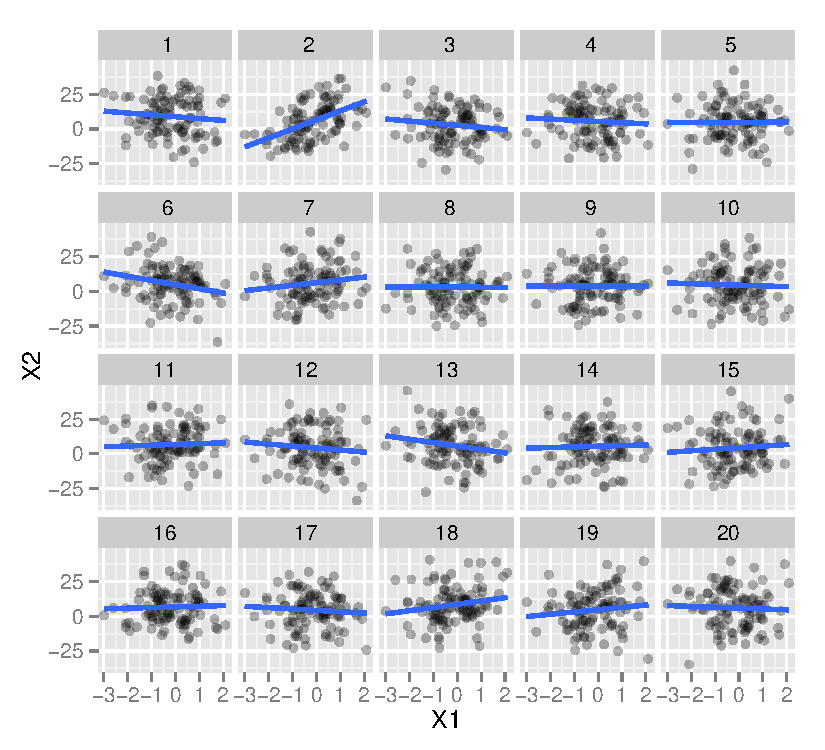
\includegraphics[width=.8\textwidth]{lineup-protocol-example.pdf}}
\caption{Example lineup plot of size $m = 20$ of scatterplots with overlaid regression line, fro a simulation study to compare the protocol with the classical $t-$test of $H_o: \beta_k = 0$, where covariate $X_k$ is continuous. One of the plots in the lineup is the plot of the pseudo-data, generated from a model where $\beta_k\neq 0$, and the others are null plots generated by simulating data from the null distribution $\beta_k = 0$. Which plot has the steepest slope? }
\label{lineup-example}
\end{figure}

Figure~\ref{compare} illustrates the difference between the classical test, and the lineup protocol, for the example shown in Figure~\ref{lineup-example}. In the lineup protocol, a finite set of draws from the sampling distribution is used for comparison, as opposed to the full distribution for the classical test. To be clear, in practice we do not know the sampling distribution -- this is a special case, where the lineup was produced under a classical scenario, and we know where the pseudo-data plot and the null plots fall in regard to the known sampling distribution. Also, in practice with crowd-sourcing many lineups can be generated, so the data plot can be compared to more than 19 nulls. The left plot shows the classical testing setup, where the null hypothesis is rejected as the calculated test statistic falls in the shaded region. In contrast, with the lineup protocol, the null hypothesis is rejected if the human observers unqeuivocally identify the data plot. In this example, we would expect the observers would identify the data plot, marked by \#~16, because it corresponds to an extreme value on the sampling distribution. 
\begin{figure}[!t]
\centering
\begin{subfigure}[t]{0.49\textwidth}
  \caption{Classical Inference}
\vspace{-.1in}
  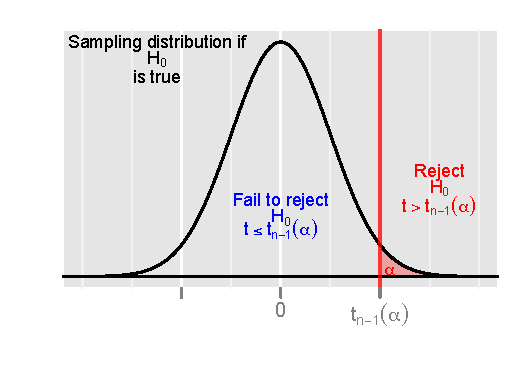
\includegraphics[width=\textwidth]{diagram.pdf}
\end{subfigure}
\begin{subfigure}[t]{0.49\textwidth}
  \caption{Visual Inference}
\vspace{-.1in}
  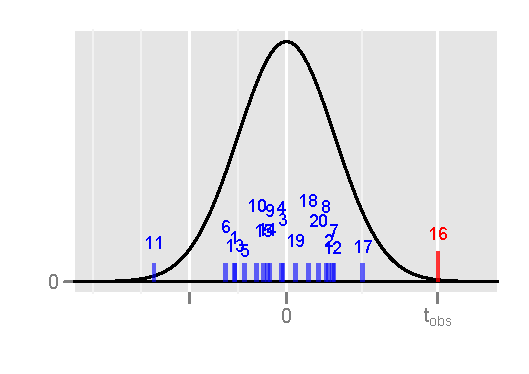
\includegraphics[width=\textwidth]{visual-inference-plot-1.pdf}
\end{subfigure}
\vspace{-.2in}
\caption{If the lineup protocol was to be used instead of classical inference this is what it would look like. (a) Rejection region (shaded in red) for classical inference for $H_0: \mu=\mu_0$ vs $H_a:\mu>\mu_0$  and (b) values corresponding to the true value (red) and the null plots (blue) in a single lineup of size $m=20$ that would be used to test the same null hypothesis.  The actual  data plot is extreme relative to the null plots, and observers would likely be able to pick it out, resulting in a decision to reject the null hypothesis. In practice, the lineup protocol would not be used if a classical test can be used. } 
\label{compare}
\end{figure}

To date, more than 20 studies have been conducted utilizing the lineup protocol, primarily using MTurk. The first three experiments (described in \citet{majumder:2011}) compared the protocol to classical tests associated with fitting linear models. A later experiment examined the use of the protocol for detecting clusters in high-dimensional data \citep{roychowdhury:2013}. Each of these experiments involved a carefully controlled study where structure in plots was generated using simulation, and multiple replicates for each treatment were used. Subjects participating in the studies were experienced MTurk workers, and evaluated blocks of ten lineups. The blocks were chosen using stratified sampling. Care was taken in the studies to ensure that each subject only saw one realization of any data. For each lineup subjects selected a plot from the lineup that they felt best matched the question asked, rated how sure they had found the best match, and why they decided on their choice.  (Full details of the experimental setups and data collection are provided in the Appendix.) It is the data from these experiments (Table \ref{tbl:visual_stat}) that we now examine with a different purpose, to assess how distance metrics compare with human evaluation. All combined, this amounts to information from 1047 subjects examining 206 lineups. The questions arising from these studies are: 

\begin{itemize} \itemsep 0in
  \item Using distance metrics applied to data plots, can we get the computer choose like a human does?
  \item Do some distance metrics match how subjects choose plots better than others?
  \item Could distance metrics be used as a first pass in designing simulation experiments for the lineup protocol to group lineups into levels of ``easy'', ``moderate'', ``difficult''?
\end{itemize}

\begin{table*}[hbtp] 
\centering 
\caption{Overview of the three MTurk experiments, from which data was extracted to investigate distance metrics in relation to subject choices. } 
\begin{tabular}{m{.8cm}m{3.25cm}m{2cm}m{.5\textwidth}} 
\hline\hline 
 ID & Experiment & Test Statistic  & Lineup question \\ [0.5ex] % inserts table %heading 
\hline 
I  & Box plot & \begin{minipage}[c]{2cm} \begin{center}	\scalebox{0.12}{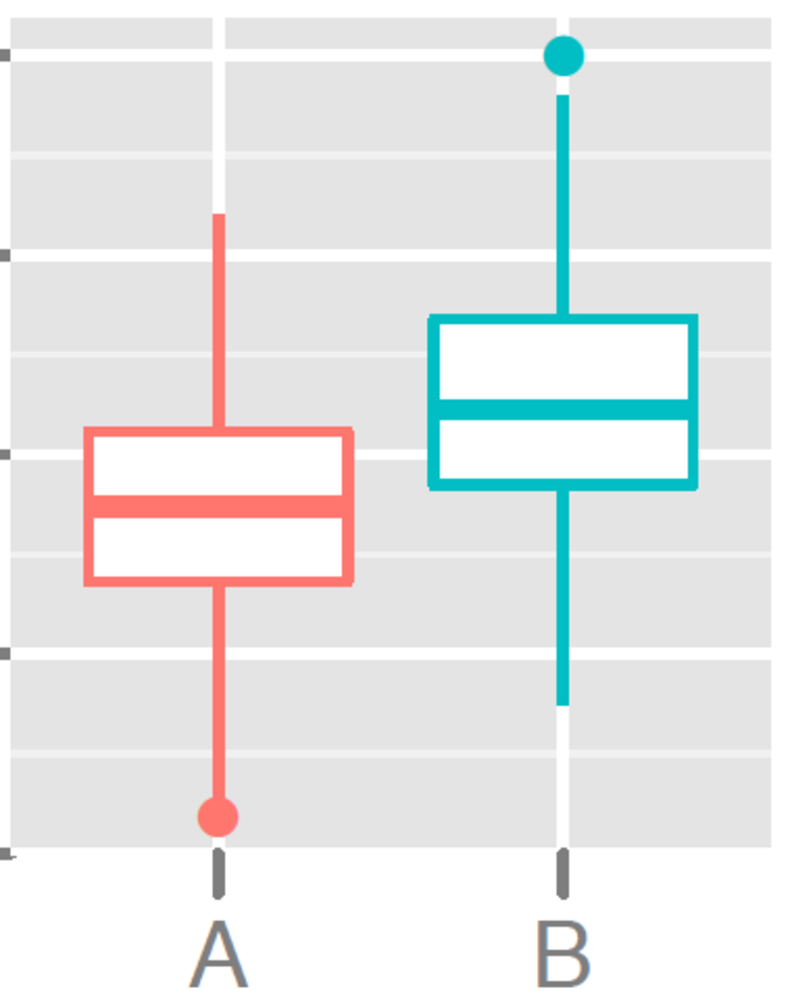
\includegraphics{stat_category1.pdf}} \end{center} \end{minipage} & Which set of box plots shows biggest vertical difference 
between group A and B? \citep{majumder:2011} \\
II &  Scatter plot & \begin{minipage}[c]{2cm}  \begin{center} \scalebox{0.3}{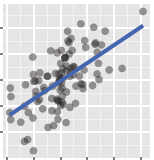
\includegraphics{stat_beta_k1.png}} \end{center} \end{minipage} & Of the scatter plots below which one shows data that has steepest slope? \citep{majumder:2011}\\
III & Group separation & \begin{minipage}[c]{2cm} \begin{center}  \scalebox{0.4}{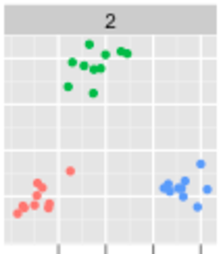
\includegraphics{stat_separation.pdf}} \end{center} \end{minipage} & Which of these plots has the most separation between the coloured groups?  \citep{roychowdhury:2013}\\
\hline 
\end{tabular}
\label{tbl:visual_stat} 
\end{table*} 

The paper is organized as follows. %Section~\ref{sec:null} discusses the null generating mechanisms. 
Section~\ref{sec:dists} starts by defining distance measures and discussing different choices of measures. The distribution of the distance measures are studied in Section~\ref{sec:distri}. Section~\ref{sec:plot_type} describes the effect of the plot type and the question of interest on the distance measure while Section~\ref{sec:eval} talks about the distance evaluations. %In Section~\ref{sec:nbin}, the methods to select the number of bins for the binned distance is described. 
Section~\ref{sec:results} presents a comparison of the distance measures to the performance of human subjects in several experiments conducted with MTurk.

%%%%%
%Graphics are an important component of big data analysis, providing a mechanism for discovering unexpected patterns in data. Pioneering research by \citet{gelman:2004}, \citet{buja:2009} and \citet{majumder:2011} provide methods to quantify the significance of discoveries made from visualizations. %Although, there have been major advances in statistical graphics over the years, for example, systems like R \citep{R} provide high quality static graphics, and very recently some access to interactive graphics. But the problem remains that graphics are not widely considered to be a part of inferential statistics. 
%\citet{buja:2009} introduced two protocols, the Rorschach and the lineup protocol, which bridge the gulf between traditional statistical inference and exploratory data analysis. The Rorschach protocol consists of a set of $m$ (usually, $m=20$) plots (called the {\it null plots}) rendered from data that is consistent with a given null model. That way, the Rorschach protocol helps to understand the extent of randomness in the null model. Under the lineup protocol, a plot of the observed data is placed randomly among a set of $m-1$ null plots.
%Human observers are then asked to  examine the lineup and to identify the most different plot. If observers identify the data plot, this is quantifiable evidence against the null hypothesis. 
%The lineup protocol places a statistical plot firmly in the framework of hypothesis tests: a plot of the data is considered to be the test statistic, which is compared against the sampling distribution under the null hypothesis represented by the null plots. 
%Obviously, the null generating mechanism, i.e.\ the method of obtaining the data for null plots, is crucial for both the lineup and the Rorschach protocol. 
%The null hypothesis directly affects the choice of null generating method. 
%Null generating methods are typically based on (a) simulation, if the null hypothesis allows us to directly specify a parametric model, (b) sampling, as for example in the case of large data sets, or (c) permutation of the original data \citep[see e.g.\ ][]{Good05}, which allows for non-parametric testing  that preserves marginal distributions  while ensuring independence in higher dimensions. 
%In the experimental data that we analyzed the null generating methods used were permutation methods and direct simulation from a null model.

%The lineup protocol was formally tested in a head-to-head comparison with the equivalent conventional test in \citet{majumder:2011}. The experiment utilized human subjects from Amazon's Mechanical Turk \citep{turk} and used simulation to control conditions. The results suggest that  visual inference is comparable to conventional tests in a controlled conventional setting. This provides support for its appropriateness for testing in real exploratory situations where no conventional test exists. Interestingly, the power of a visual test increases with the number of observers engaged to evaluate lineups, and the pattern in results suggests that the power will provide results consistent with practical significance \citep{kirk:1996}.


%Figure~\ref{lineup-example} gives an example of one of the lineups used in a head-to-head comparison with classical testing (results are discussed in more detail in section~\ref{sec:turk2}). 
%
%Suppose we have the following statistical model
%
%$$Y_i = \beta_0 + \beta_1 X_{i1} + \beta_2 X_{i2} + \dots + \epsilon_i$$
%
%\noindent and we are interested in testing the following hypothesis:
%
%$$H_o : \beta_k = 0 \qquad \qquad \hbox{vs} \qquad \qquad H_A: \beta_k \ne 0$$
%
%\noindent where $X_k$ is a continuous covariate. Assume, the data plot is a scatterplot of $Y$ against $X_k$ with a regression line overlaid. We can generate null plots from rendering simulating data from $N(X\hat{\beta}, \hat{\sigma}^2)$ and plotting using the same scatterplot method as the true data, where parameter estimates ($\hat{\beta}, \hat{\sigma}^2$) are obtained by fitting the null model to the true data. 
%The plot of the true data is randomly placed among a set of ($m$ - 1) null plots to produce a lineup of size $m$. Rather than to identify the most different plot, human subjects are asked to identify the plot with the steepest slope from the lineup of Figure~\ref{lineup-example}. If the human subjects can identify the plot of the true data, we reject the null hypothesis and conclude that there is a significant linear relationship between $Y$ and $X_k$. 
%For the example of this lineup sum(lpu$response) out of nrow(lpu) observers correctly identify plot~\#2 as the data plot, providing very strong evidence of a linear relationship.

%In traditional hypothesis testing, the sampling distribution of a test statistic is functional and continuous. In the lineup protocol, although conceptually we may have an infinite collection of plots from the null distribution, in practice, we can only evaluate against a finite number of null plots. A human judge has a physical limit on the number of plots they can peruse. This poses one of the issues with using the lineup protocol.  Figure~\ref{compare} illustrates the difference. In traditional inference, the black curve represents the sampling distribution for the $t$-distribution under the null hypothesis, and the shaded red area shows the rejection region. 


%Plots are used as test statistics in visual inference, which are, unlike their traditional counterparts, not simple numbers but more complex entities. We can, however, calculate the value of the test statistic based on the data underlying the true plot, as well as the corresponding value for each of the null plots.
%These values are shown using the red bar (data plot) and the blue bars (null plots) in Figure~\ref{compare}.
%Effectively,  in visual inference the red line is compared  to only these finite number of blue lines  to make a decision, unlike classical inference where we look at the rejection region (Figure~\ref{compare}) to make decisions. Even though the data plot might be extreme, it is possible by randomly selecting from the null distribution, to obtain a null plot that is more extreme, as Tukey suggested \citep{fernholz03}:

%\begin{quotation}
%``There [in Tukey's Data Analysis class] I discovered that [...]  a random sample is indeed a ``batch of values'' which ``fail to be utopian'' most of the time.''
%\end{quotation}


%{\color{red}***Point 2: Use metrics to ensure that a range of comparisons is made available to observers}

%This can be partially solved by having a large number of observers, who each evaluate lineups constructed using different null plots. Having some idea of the type of coverage of the sampling distribution that is provided by the lineups would be useful ahead of engaging observers and evaluating the lineups. Could we say that lineup X is expected to be ``difficult'' but lineup Y is expected to be ``easy''? This information might then help in  planning other aspects of the experiment such as e.g.\ determining an appropriate number of observers. Intuitively, a difficult lineup is one where the data plot is similar to the null plots, while the data plot in an easy lineup  has some feature that makes it stand out from the null plots. Being able to compute a distance metric based on features of the plot would be very helpful ahead of running a lineup protocol.

%Researchers needs to provide a range of comparisons to observers to judge. An efficient design of experiment would be to provide a range of lineup plots with varying difficulty to the human subjects to look at. So far the difficulty of a lineup can be evaluated based on the performance of the subjects. The performance of the subjects can be analyzed after the experiment. But as a researcher, it would be interesting to have an idea about the difficulty of the lineups even before the experiment is conducted so the subjects see a set of lineups with varying difficulty. Distance metrics can be of great help in this case. 


%To avoid basing conclusions on artifacts introduced by a `bad' sample, we need to be aware of properties of this set of null plots. In this paper, we develop techniques that help to determine the quality of the lineup. A variety of distance metrics measuring the ``closeness'' of the true data plot and the null plots, and the null plots with themselves are examined. These are compared to human subject picks in several Amazon Turk studies.  Describing plots numerically, is something  of an oxymoron, it cannot be done. Nonetheless, the distance measures provide indications of the quality of a lineup. The purpose of this paper is to help determine if a lineup might provide inadequate coverage of the full null distribution, and these measures might help to gain more insight on how the human eyes work in reading statistical graphics. 

%{\color{red} ***  Point 3: Metrics might replace human observers, eventually, but as of now, human eye can still beat numbers for finding unexpected patterns. The lineup protocol gives us a chance to evaluate metrics to finding unexpected structures - check out the scagnostics literature}

%This is a two way process: As metrics are devised to measure the quality of a lineup, the lineup protocol also provides an opportunity to measure the performance of a metric. The human eye can detect patterns in a plot that cannot be easily quantified numerically, which is why graphics provide an important tool for exploring data and finding the unexpected. Describing plots numerically, is something  of an oxymoron, it cannot be universally done. An example of past work are {\it scagnostics}, short for scatterplot cognostics \citep{tukey:1977}, which were further investigated in form of graph-based scagnostics \citep{wilkinson2005graph}. Both attempt to assess various aspects of scattered points like outliers, shape, trend, density and coherence.  If a scatterplot has just one of these structures the scagnostics are descriptive, however, they fail terribly if a plot contains more than one or an unforeseen feature instead. The goal here is to find  distance measures that can provide an indication of the quality of a lineup, and then to use the results of observer evaluation to determine which metrics best reflect what features of a plot people see and assess for their choice.

%{\color{red} *** Point 4: Metrics can help us understand what it is that people pick up on to trigger a detection of the data. Currently lineups rely on people verbally reporting why they picked a plot. }

%Following up on choices, observers are asked to describe their reasoning. These reasons are used to obtain more information about the rejection: was it some nonlinear dependency, an outlier, clustering or something else that triggered the detection of the data plot? Good distance metrics may also help to relate the descriptive words used to mathematically defined features. 

%The article is organized as follows. %Section~\ref{sec:null} discusses the null generating mechanisms. 
%Section~\ref{sec:dists} starts by  defining distance measures and discussing different choices of measures (see Section~\ref{sec:meas}). The distribution of the distance measures are studied in Section~\ref{sec:distri}. Section~\ref{sec:plot_type} describes the effect of the plot type and the question of interest on the distance measure while Section~\ref{sec:eval} talks about the distance evaluations. %In Section~\ref{sec:nbin}, the methods to select the number of bins for the binned distance is described. 
%Section~\ref{sec:results} presents a comparison of the distance measures to the performance of human subjects in several experiments conducted by Amazon's Mechanical Turk.

% We also calculate the distance matrices between the null plots to see how close are the null plots to each often. Finally a percentile value is calculated to find how often such a distance appears in a lineup and a z-score of the different distances is calculated to get a measure on the closeness between the null plot and the actual plot and also compare between two different lineups.  


%\red{the next three paragraphs might be important, but you loose focus - you want to come as fast as possible to the problematic of the paper, e.g.:}

%For two different visual test statistics of the same true data, the one  is better, in which a specific pattern is more easily distinguishable visually. \\ \\

%\red{Before distance measures are introduced, introduce the problem of why we look at these distances in the context of permutation tests. }
%The difference between a regular permutation test and a graphical test under the line-up protocol, is that we are comparing the true value of the test statistics (i.e. the plot of the true data) to a finite sample of the sample distribution.

%{\color{red} Things to add:
%\begin{enumerate}
%\item Null-generating mechanisms  
% \hh{sorry, I guess I interfered with that - I moved pieces of the section on null generating mechanism into the intro and some into the discussion of the results.}
%\item Dependence on Question of Interest - in general should not be a problem because the question is ``which is different? ". But for data from Turk study, questions were quite focussed.
%\item Interplay between type of plot and distance metric - calculation on data vs graphical elements. For example, scatterplot vs reg line distance
%\item Distance metric distribution calculation eg permutation
%\item Selection of the number of bins
%\end{enumerate}}


% \section{Null Generating Mechanism} \label{sec:null}
% 
% \hh{XXX at the moment this section is not fitting in properly: it is too long and detailed to go into the intro, but it does not contain novel work to allow to go at a later point. I would suggest to extract a small paragraph on the importance of the null generating mechanism for the intro and  a detailed discussion of the null generating mechanism used at the beginning of each subsection in the experiments. XXX}
% 
% The lineup protocol embeds the true data plot among a set of null plots. The method of obtaining the data for these null plots is called the null generating mechanism. %These null plots are obtained from the null distribution in a method consistent with the null hypothesis. 
% The null hypothesis directly affects the choice of null generating method. In the experimental data that we analyzed the null generating methods used were:
% \begin{enumerate}
% \item {\bf Permutation:} Because of its versatility, this is a commonly used apporach. Permutation is used to break the association between two or more variables, and thus is appropriate when the null hypothesis is that there is no association. Consider two variables $X_1$ and $X_2$. Either $X_1$ or $X_2$ is permuted while keeping the other variable fixed. Any association between $X_1$ and $X_2$ is broken in the process altering the joint distribution between the variables, whereas the marginals of $X_1$ and $X_2$ remains the same. The method works in situations where one or both the variables are continuous or categorical. Let us consider a case where we have one categorical variable, say, Group and a continuous variable. Let us assume that the variable Group has two levels (say, A and B) and we want to test whether there is any significant difference between the two groups, i.e.\ $H_o: \mu_A = \mu_B$. To generate the null data, the values of the variable Group are permuted keeping the continuous variable fixed. If there is a difference between the two groups, this difference is broken by the permutation, and any difference observed in the permuted data is consistent with random variation.
% \item {\bf Simulation under a null model:} Sometimes there is a model underlying the problem being studied. In this situation simulating from the model will be the null generating mechanism.  The parameter estimates are obtained from  fitting  the model to the true data. Data is then generated using the parameter estimates. Let us assume that we are interested in testing whether there is any significant linear relationship between two continuous variables $X_1$ and $X_2$. Hence, we test for $H_o : \beta_1 = 0$ versus $H_a: \beta_1 \ne 0$. Under the null hypothesis, we fit the following model to the data:
% $$Y = \beta_0 + \varepsilon$$
% where $\varepsilon \sim N(0, \sigma^2)$. The parameter estimates of $\beta_0$ and $\sigma^2$ are obtained and null data is generated from $N(\widehat{\beta_0}, \widehat{\sigma}^2)$. 
% %\item \red{*** Not used by us, so exclude for now} Simulation from a specific distribution:  When the null hypothesis is that the data comes from a specific distribution, this distribution can be used to simulate new samples that generate the null plots. The parameters for the null distribution are obtained from the estimates calculated using the data. For example, suppose we want to test whether data comes from a Normal distribution, $H_o:$ data $\sim$ Normal vs. $H_A:$ data $\nsim$ Normal, then the null data are generated from the Normal distribution with mean and standard deviation equal to the estimated mean and standard deviation from the data. 
% \end{enumerate} 

%Other null generating mechanisms might be utilized depending on the null hypothesis underlying a data plot. 

\section{Distance Measures}\label{sec:dists}
%\subsection{} \label{sec:meas}
The goal of the metrics is to measure the ``distance'' between two plots. In particular, we would like to know how similar or different is the data plot from the surrounding null plots. 

A naive approach would be to use existing goodness-of-fit statistics that compare data with reference probability distributions, for example, the Kolmogorov-Smirnov \citep{stephens:1974}, Anderson-Darling \citep{stephens:1974}, Shapiro-Wilk \citep{shapiro:1965} tests and Bhattacharyya distance \citep{bhattacharyya:1946}. However, these measure differences between univariate distributions which limits their applicability to distances between plots, generally. Bhattacharyya distance is used for image processing but not in manner useful for plot comparisons.
%By calculating the ``distance'' between plots we may be able to determine if a lineup should be easy -- if the actual data plot is detectably different from the null plots -- and also to better understand what aspect of the plot people use to make their choice. It is not an easy task to measure the difference between plots. Here we examine several possibilities. 
%The problem could be tackled by considering the data as a reference distribution, and compare all of the null sets with this reference. Comparing data with a reference probability distribution or comparing two datasets are common statistical tasks. For example, the Kolmogorov-Smirnov test \citep{stephens:1974} sorts values in two samples, computes the empirical distribution function of each and compares these two, to determine if the two samples are likely to have come from the same distribution.  The Anderson-Darling \citep{stephens:1974} and Shapiro-Wilk \citep{shapiro:1965} tests compare datasets with normal probability distributions. These measure differences between univariate distributions which limits their applicability to distances between plots, generally. 
Hausdorff distance \citep{huttenlocher:1993} has been successfully used for comparing images. It effectively matches points between sets and computes the distances between the matched points, but it is prohibitive computationally. 

Along these lines, \citet{hannig:2013} developed a metric for comparing two images, based on one developed by \citet{Baddeley:1992}. Comparing two images is different from comparing two data plots, where only essential plot elements are compared, so this metric is not useful comparing data plots generally. \citet{marron:1995} describes metrics for comparing two curves developed because the results from smoothing, based on classical mathematical norms do not match how the eye perceives the difference. This is too specialized. Actually, the lineup protocol could be utilized to rigorously substantiate the work in these papers. 

In many practical uses of the lineup protocol, permutation can be used to generate data for the null plots in a lineup. This was employed in the study done in experiment III. Hamming distance \citep{hamming:1950} calculates how different the permutations are, by measuring the minimum number of substitutions it takes to get from one permutation to another. It was one of our initial choices of distances, but it did not do well at distinguishing data plots from null plots, probably because it does not compare differences between the actual numbers, so we abandoned it. 

Interpoint distance metrics, developed for cluster analysis, are fast to compute. These can be adapted to measuring structure in plots. For example, when the purpose is to compare two scatterplots containing clusters, we might calculate the smallest intercluster distance for both plots, and then use this to determine which plot exhibits the strongest clustering. This distance, together with various other measures to calculate distances between groups is implemented in the R package {\tt fpc} \citep{hennig:2010}. Figure~\ref{sep-dist} illustrates choices of metrics for measuring clustering. These are especially applicable to data from experiment III. The method can be adapted more broadly to different types of plots. For example, to measure the structure in a graph of side-by-side boxplots of two groups. The graphical features of the plot are the two five number summaries represented by the boxplots. An interpoint distance measuring the difference between the two sets of five points, can determine which plot exhibits the biggest difference between the two groups.

\begin{figure}[!t]

\centering
\begin{subfigure}[t]{0.24\textwidth}
\caption{\label{type1_minsep} \scalebox{0.8}{Minimum Separation}}
%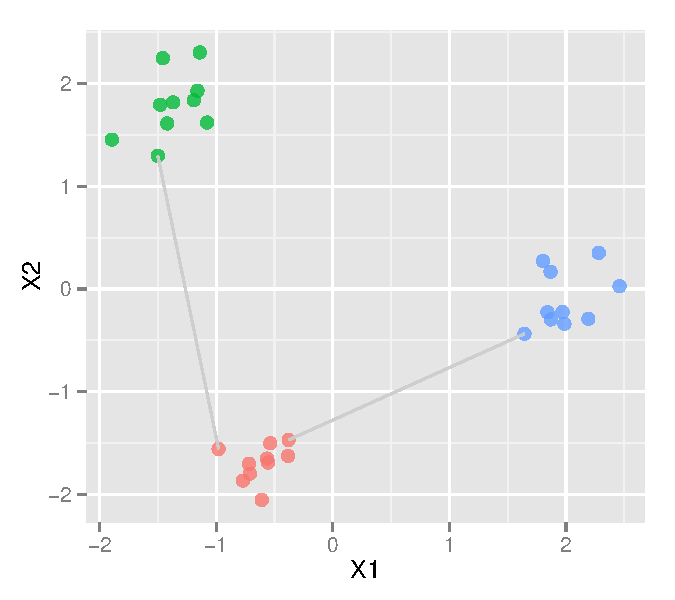
\includegraphics[width=\textwidth]{min-sep-example.pdf}
\begin{knitrout}
\definecolor{shadecolor}{rgb}{0.969, 0.969, 0.969}\color{fgcolor}
\includegraphics[width=\textwidth]{figure/min_sep_ex-1} 

\end{knitrout}
\end{subfigure}
\begin{subfigure}[t]{0.24\textwidth}
\caption{\scalebox{0.8}{Average Separation}\label{type_2_avesep}}
%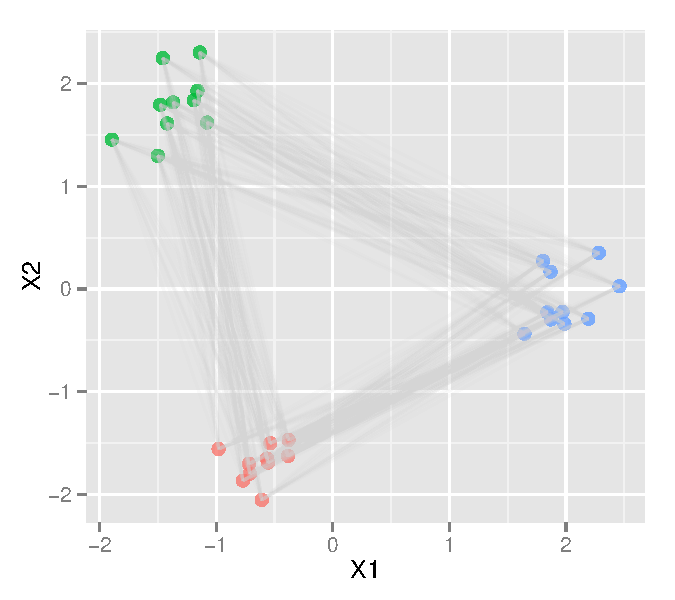
\includegraphics[width=\textwidth]{ave-sep-example.pdf}
\begin{knitrout}
\definecolor{shadecolor}{rgb}{0.969, 0.969, 0.969}\color{fgcolor}
\includegraphics[width=\textwidth]{figure/ave_sep_ex-1} 

\end{knitrout}
\end{subfigure}
\begin{subfigure}[t]{0.24\textwidth}
\caption{\scalebox{0.8}{Cluster Mean Sep.}\label{type_2_clsep}}
%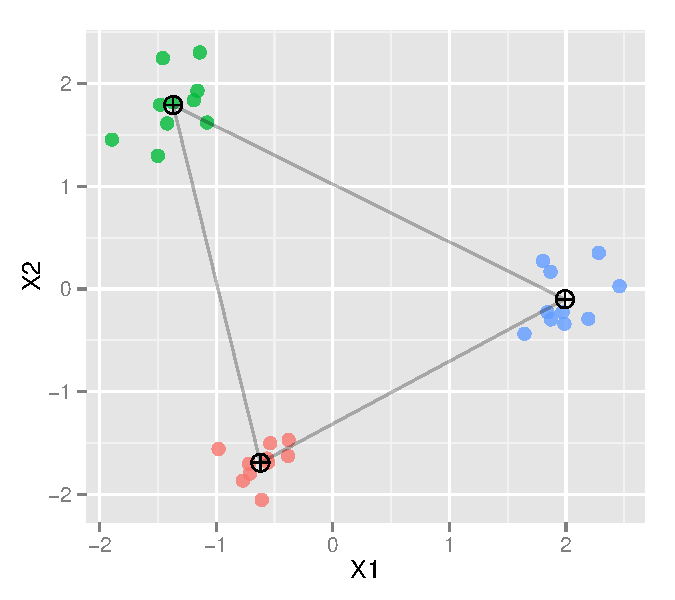
\includegraphics[width=\textwidth]{mean-sep-example.pdf}
\begin{knitrout}
\definecolor{shadecolor}{rgb}{0.969, 0.969, 0.969}\color{fgcolor}
\includegraphics[width=\textwidth]{figure/cm_sep_ex-1} 

\end{knitrout}
\end{subfigure}
\begin{subfigure}[t]{0.24\textwidth}
\caption{\scalebox{0.8}{Dunn Index}\label{type_2_dunn}}
\vfill
%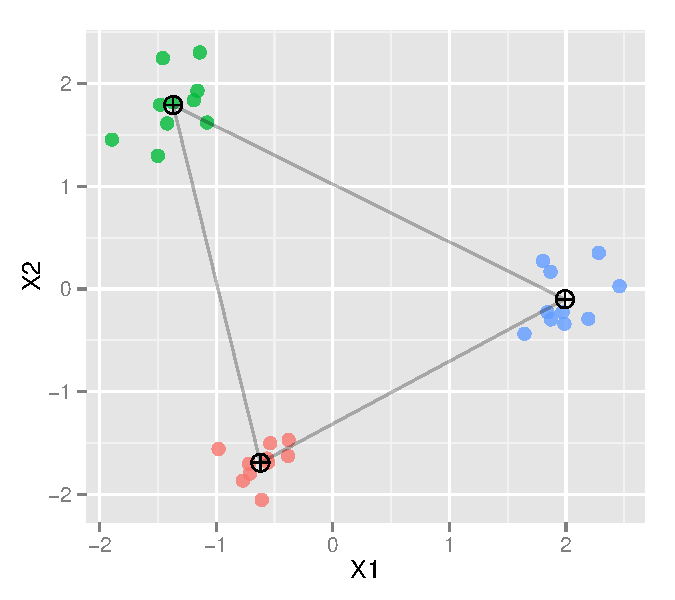
\includegraphics[width=\textwidth]{mean-sep-example.pdf}
\begin{knitrout}
\definecolor{shadecolor}{rgb}{0.969, 0.969, 0.969}\color{fgcolor}
\includegraphics[width=\textwidth]{figure/di_sep_ex-1} 

\end{knitrout}
\end{subfigure}

	\vspace{-.1in}
\caption{Illustration of four different distance metrics for cluster separation. Minimum Separation (a) calculates the minimum distance between points of each cluster from the other clusters. Average separation (b) calculates the average distance of each point in a cluster to the other clusters. Cluster mean distance (c) sums the distances between the means of each cluster. The Dunn index (d) is based on a comparison of minimal separation between clusters (as shown in  (a)) and maximal cluster diameter.}
\label{sep-dist}
%{Caption of subfigures \subref{fig:subfig1}, \subref{fig:subfig2} and \subref{fig:subfig3}}
\end{figure}


%two graphs containing side-by-side boxplots, a distance metric that focuses on group separation calculated on each data set might be useful. Bhattacharyya distance \citep{bhattacharyya:1946} is widely used in image processing, for feature extraction. This distance, together with various other measures to calculate distances between groups is implemented in the R package {\tt fpc} \citep{hennig:2010}. % contains many different ways to calculate distances between groups. 

After trialing many of these distance, we report on the results from just a few metrics, that performed best. One approach was the interpoint distances, adapted to the displays used in experiments I-III, and the other a simple relatively simple distance based on binned frequencies (illustrated by Figure \ref{first-example}), which is generalizable to most data plots. 
%In the analyses of the experimental data of this paper, we used a dual approach: one distance that we employed for all examples is a relatively simple distance based on binned frequencies, which works fairly well in most circumstances.
%Ultimately, a very simple binned distance was used in the analyses of the MTurk data, which worked fairly well in most circumstances. 
%However, it was clear immediately that plot design, and the question asked, has a large impact on how a plot is read, and specific distance metrics designed for specific plot types and tasks are needed. In order to more closely reflect observers' choices in each experiment, we used at least one more distance tailored to each of these special situations.
A summary of distance metrics follows, along with a procedure for computing the empirical distribution of the distance metrics, that can is used to measure the distance between data plot and null plots. 

\begin{figure*}[!t]
\centering
\begin{subfigure}[t]{\textwidth}
\caption{Dataset $X$ with two variables $X_1$ and $X_2$ \label{type_1}}
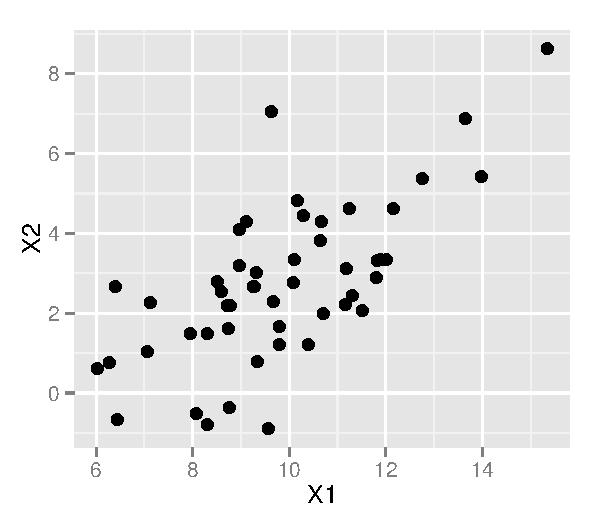
\includegraphics[scale=0.55]{dat-example-1.pdf}
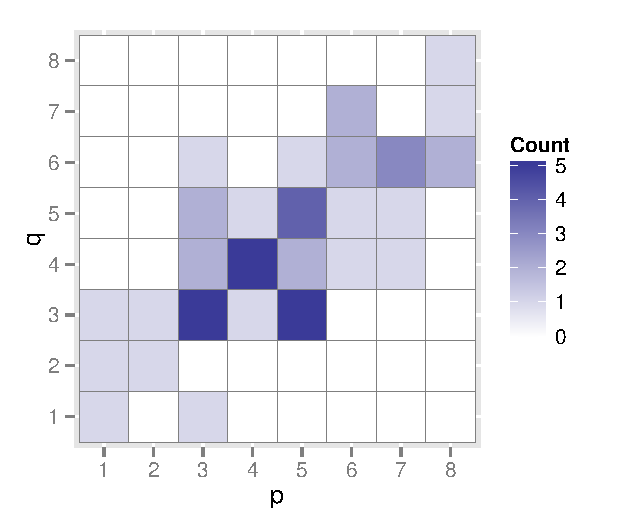
\includegraphics[scale=0.55]{bin-example-1.pdf}
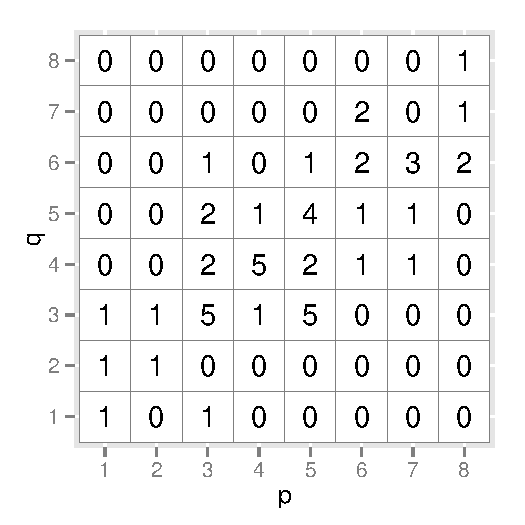
\includegraphics[scale=0.55]{freq-example-1.pdf}
\end{subfigure}

\begin{subfigure}[t]{\textwidth}
\caption{ Dataset $Y$ with permuted $X_1$ and original $X_2$ \label{type_2}}
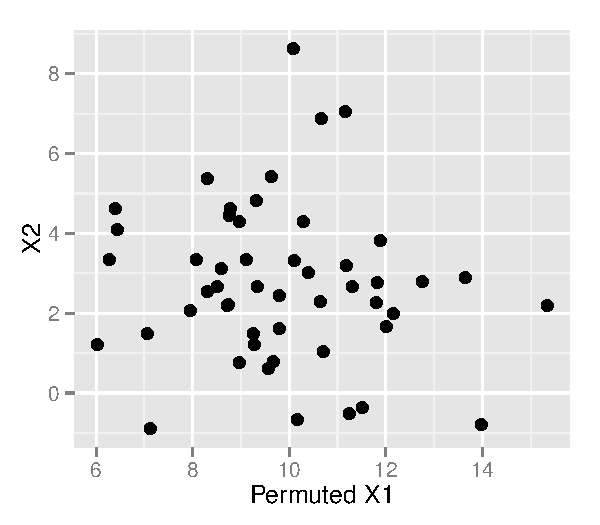
\includegraphics[scale=0.55]{dat-example-2.pdf}
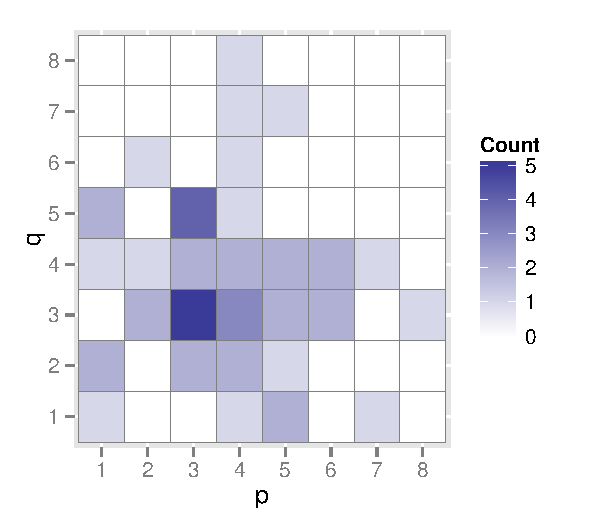
\includegraphics[scale=0.55]{bin-example-2.pdf}
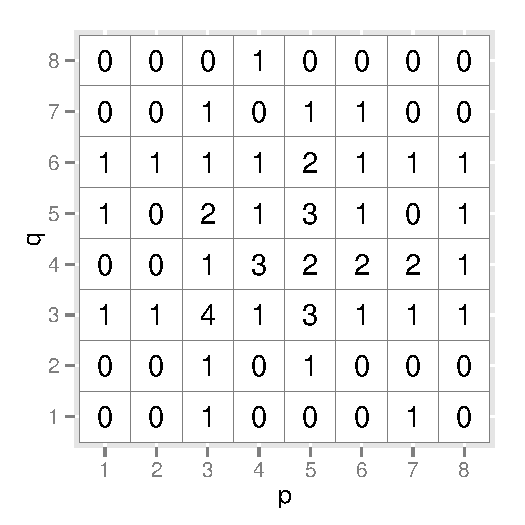
\includegraphics[scale=0.55]{freq-example-2.pdf}
\end{subfigure}
\label{first-example}
	\vspace{-.1in}
       \caption{Illustration of binned distance for data with a strong positive association (a), and the same data where variable $X_1$ has been permuted (b). The scatterplot of the data is shown (left) along with a binned view of the data (center) and the cell count matrix $C$ (right). Binned distance is the Euclidean distance of these counts. The binned distance between these plots is 6.4807. }
\label{first-example}
%{Caption of subfigures \subref{fig:subfig1}, \subref{fig:subfig2} and \subref{fig:subfig3}}
\end{figure*}

\subsection{Distance metrics}\label{sec:distmet}

A sketch of the distance metrics is provided here, with full details available in the Appendix.

\begin{enumerate}

\item {\bf Binned Distance (BN):} compares the cell counts from binned data. This distance can be calculated for univariate continuous data, bivariate data with two categorical variables, or data with one continuous and one categorical variable. For a categorical variable, we choose the number of bins  to be equal to the number of categories.

Binned distance is highly susceptible to small differences in values and depends on the number of bins as well as the anchor point (bottom left corner of first cell). It is necessary to find the optimal number of bins in each direction. For our purposes `optimal' was defined as the number of bins that produced the largest detectable difference between data plot  and null plots, compared to the biggest difference between any pair of null plots. Details of these choices on various different data sets can be found in the Appendix.

Several variations to this distance are possible, such as a change to using kernel density estimates, a change from $L_2$ to $L_p$ based distance, or using transformations on the counts. All of these changes will affect distances, and might lead to qualitatively different conclusions.
Hausdorff distance \citep{huttenlocher:1993} was also examined, but the binned distance is computationally efficient and performed as well as the Hausdorff as a rough, generic measure of similarity of plots.

\item {\bf Distance based on boxplots (BX):} is specifically designed for side-by-side boxplots based on only their graphical elements corresponding to the three points defining the boxes of a boxplot. It makes the assumption that subjects focus on the difference in the boxes. Variations on this might include adding whiskers' values, the number or values of outliers, or including higher-order letter values \citep{tukey:1977, lvplot} for more exact tail specifications. 

\item {\bf Distance based on the regression line (RG):} Many times, to examine association between two variables a regression line is overplotted on the points of a scatterplot. This distance was developed to help assess if the observer is paying attention to the line or the spread of points. The metric bins the data, and compares the intercept and slope of the regression line computed in the bins. Variations might include using slope alone, or absolute value of slope. 
\item {\bf Distance based on separation between multiple groups (MS, AS, DS, CM):} using minimum separation (MS), average separation (AS), Dunn separation (DS) and distance between cluster means (CM) are considered. 
\end{enumerate}


% How well each distance measure matches the observers' responses depends  on the question of interest.  
% But, in general, this should not be a problem because the question which is typically asked is ``Which plot among these is different?''. In the MTurk experiments, more focused questions were asked because the purpose was very specific, to compare visual inference with classical inference.
% 
% \hh{XXX wouldn't a more tailored question be easier to match with a tailored distance? }

Generally to compare different distance measures their empirical distribution are used.

\subsection{Empirical Distribution of Distance Metrics} \label{sec:distri}

For a given lineup of size $m$, the empirical distribution of distance metrics is obtained by calculating the distances between the null plots among themselves. One null data is generated using the null generating mechanism, and labelled to be the ``true'' data set, then a number of null data sets are generated and the distances between these datasets are calculated. Averaging all these distances yields one single distance value. This process is repeated a large number of times, say, $N$ between 1,000 to 10,000. Finally $N$ mean or average distances are obtained which gives the empirical distribution of the distance. For comparing data plot with nulls using the empirical distribution of the distance metric, we use the following algorithm:

\begin{enumerate} \itemsep 0in
\item Calculate the distance between the true data and all the null datasets and take the average of these distances. 

\item For each of the ($m$ - 1) null datasets, calculate the distance between the null data and all the other ($m$ - 2) null datasets and obtain the average distance. Hence, we obtain ($m$ - 1) distances, one corresponding to each  null plot.

\item Generate a lineup of size $m$ using the null generating mechanism. 
Single out one of these nulls as the `data' plot, and calculate the distances as described in steps (1) and (2). Repeat this procedure $N$ times.

\item The $N$ distance values then represent the empirical distribution of the distance metric and are used for making comparisons
\end{enumerate}

The observed test statistic is  compared to the empirical distribution, as shown in Figure~\ref{compare}. The distance measures for the true dataset and the null datasets are plotted on the empirical distribution. If the distance measure of the true plot is larger than any of the null plots, the lineup might be regarded as ``easy''. Otherwise, we consider it to be a ``difficult'' lineup. For easy lineups, we would expect that most observers could detect the true data plot amongst the decoys, but that far fewer observers to be able to do so with a difficult lineup. This gives us a way to compare the actual results from the MTurk human subject studies with what we might expect given the distance metric assessment.

The empirical distribution of the distance based on regression is shown in Figure~\ref{fig:distances} using $N = 1000$ simulation runs. 
Figure~\ref{dist_1} shows the lineup plot for $m = 20$ for testing whether there exists a significant linear relationship between $X_1$ and $X_2$. The 19 null plots are generated by fitting the null model and generating from the null model. Figure~\ref{dist_2} shows the general empirical distribution of distance measures based on the null model. For the particular lineup on the left, mean distances  are shown by overlaid line segments for the true plot (in orange) and the null plots (in black). The true plot is easily identifiable from the lineup (Figure~\ref{dist_1}, in the experiment 40 out of 45 observers identified the data). This is backed by the regression based distance measure seen in Figure~\ref{dist_2}, as the orange line is on the extreme right tail compared to the black lines. 

\begin{figure}[!p]
\centering
\begin{subfigure}[b]{0.55\textwidth}
\caption{\label{dist_1}Lineup: which slope is the steepest?}
%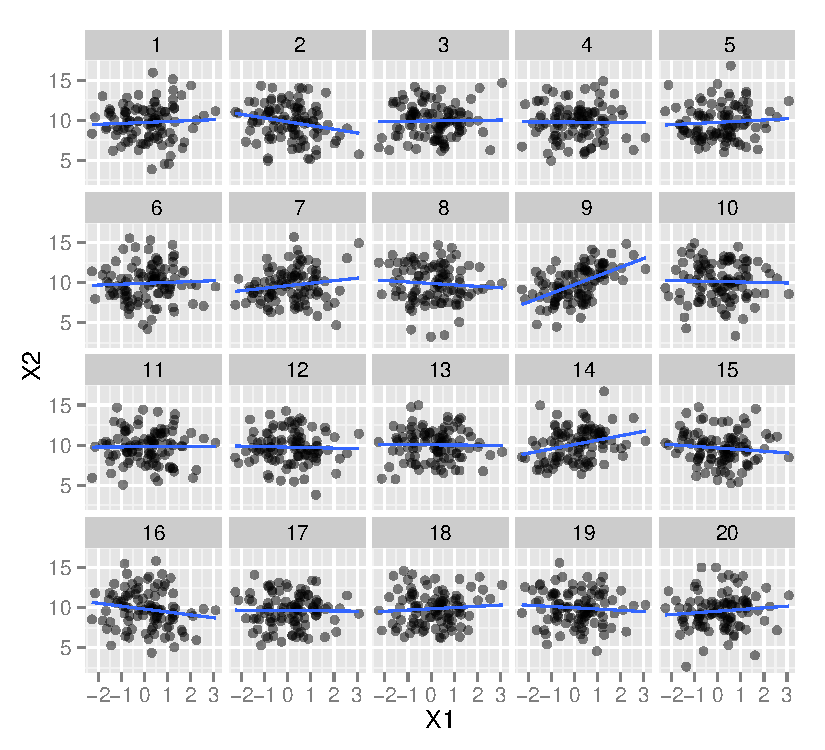
\includegraphics[width=\textwidth]{dist-example.pdf}
\begin{knitrout}
\definecolor{shadecolor}{rgb}{0.969, 0.969, 0.969}\color{fgcolor}
\includegraphics[width=\textwidth]{figure/lp-reg-1} 

\end{knitrout}
\end{subfigure}
\begin{subfigure}[b]{0.44\textwidth}
\caption{\label{dist_2}Regression based distance metrics.
%: unscaled at the top, scaled at the bottom. \hh{XXX my suggestion would be to switch to the scaled regression based distance instead of the unscaled one.} \hh{XXX I did the switch; the top density is  now the only one in the paper, that is unscaled -- this makes most of the regression based distance with the slope only superfluous.}
}
%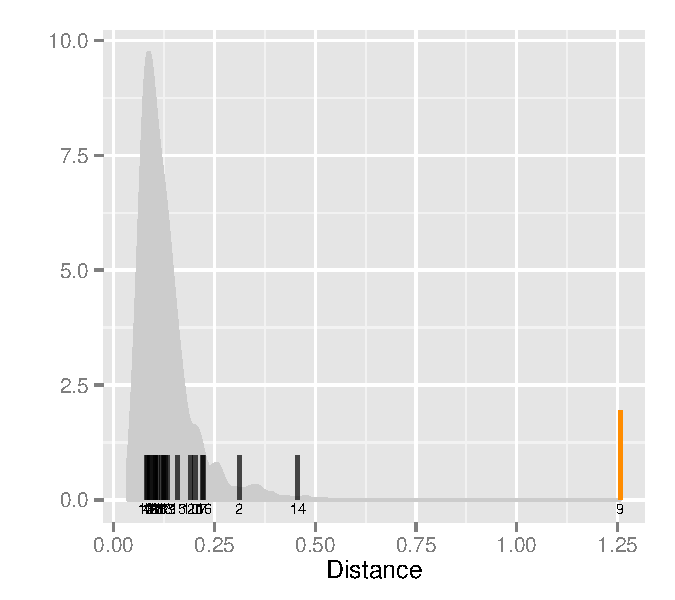
\includegraphics[width=\textwidth]{dist-metric.pdf}




\begin{knitrout}
\definecolor{shadecolor}{rgb}{0.969, 0.969, 0.969}\color{fgcolor}
\includegraphics[width=\textwidth]{figure/dens-reg-dist-1} 

\end{knitrout}
\end{subfigure}
\label{dist}
	\vspace{-.1in}
\caption{
\label{fig:distances}Illustration of the behavior of a distance metric with a lineup plot in (a) and the distribution of regression based distance metric in (b). A lineup of size $m$ = 20 is shown (left) for testing whether there exists a significant linear relationship between $X_1$ and $X_2$. The 19 null plots are obtained by simulating from the null model.  The empirical distribution of the distance metric is shown on the right and overlaid by vertical line segments for the true plot and the null plots (in orange and black, respectively).  }
%{Caption of subfigures \subref{fig:subfig1}, \subref{fig:subfig2} and \subref{fig:subfig3}}
\end{figure}

\begin{figure}[!p]
\centering
\begin{subfigure}[b]{0.55\textwidth}
\caption{\label{box-1}Lineup: which of these pairs of boxplots shows the biggest vertical difference?}
%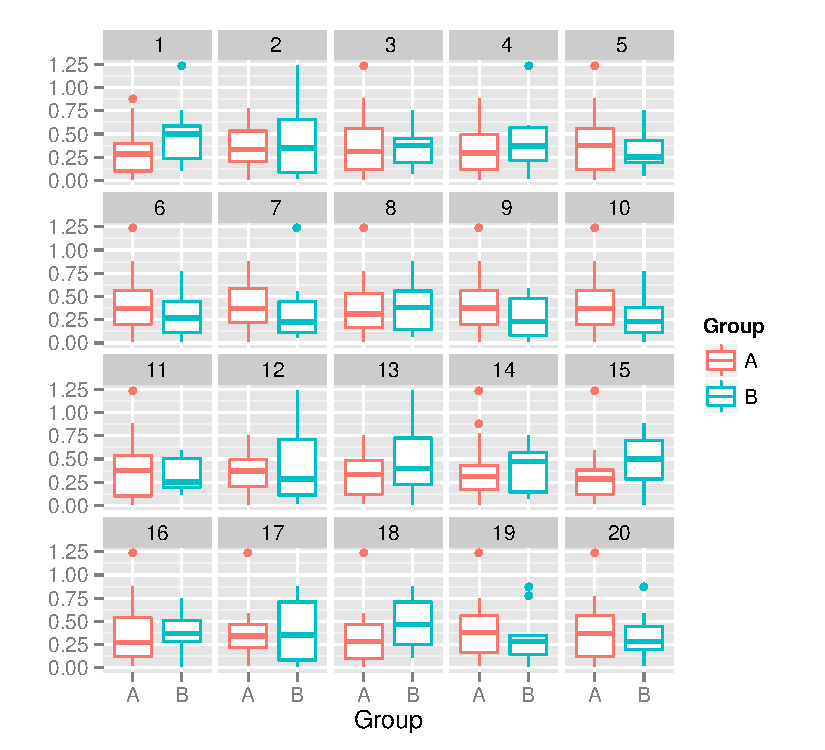
\includegraphics[width=\textwidth]{dist-example-2.pdf}
\begin{knitrout}
\definecolor{shadecolor}{rgb}{0.969, 0.969, 0.969}\color{fgcolor}
\includegraphics[width=\textwidth]{figure/lp-box-1} 

\end{knitrout}
\end{subfigure}
\begin{subfigure}[b]{0.44\textwidth}
\caption{\label{box-2}Boxplot based distance}
%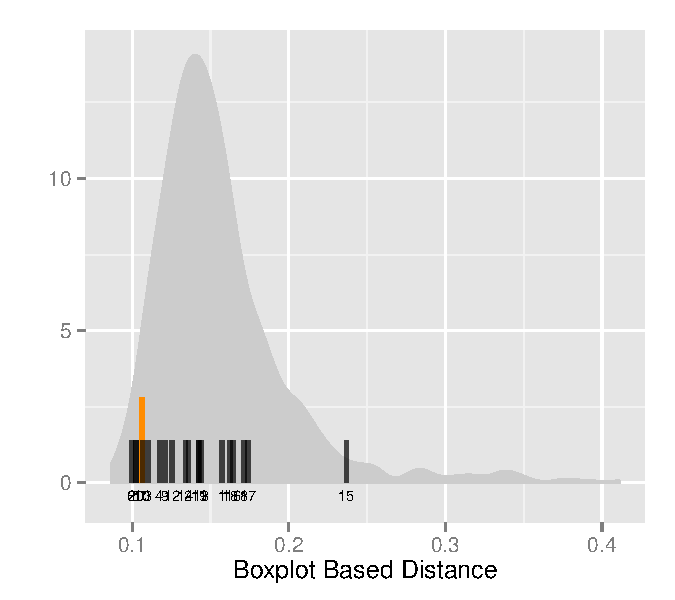
\includegraphics[width=\textwidth]{dist-metric-2.pdf}




\begin{knitrout}
\definecolor{shadecolor}{rgb}{0.969, 0.969, 0.969}\color{fgcolor}
\includegraphics[width=\textwidth]{figure/lp-box-dist-1} 

\end{knitrout}
\end{subfigure}
	\vspace{-.3in}
\caption{\label{fig:boxes} Illustration of the behavior of a distance metric for a more `difficult' lineup. The lineup is shown in (a), the density plot on the right shows the boxplot based distance metric. Of interest is whether there exists a significant shift between the two groups. The orange line (boxplot distance of the true plot) is among the black lines of the nulls, indicating that the boxes in the true plot show no more difference than a null plot from other null plots. }
%{Caption of subfigures \subref{fig:subfig1}, \subref{fig:subfig2} and \subref{fig:subfig3}}
\end{figure}

Figure~\ref{box-1} shows a lineup of size $m = 20$ for testing whether there exists a significant difference in the group medians between A and B. The 19 null plots are generated from a null model, consisting of draws from a normal distribution.  Figure~\ref{box-2} shows the empirical distribution of the distance based on the boxplots with the mean distance for the true plot (in orange) and the null plots (in black). It is hard to identify the true plot from the lineup. During the study, only 2 out of 26 observers picked the data plot, indicating little to no evidence of a deviation from the null hypothesis. This  is also evident from the boxplot based distance measure: the orange line corresponding to the true data is mixed in with the mass of the black lines, with one null plot (16) exhibiting a lot more signal than the true plot.

\subsection{Metric Evaluation} \label{sec:eval}
%
For a lineup of size $m = 20$, the average distance of the true plot from all null plots is compared to 18 average distances between the null plots. This high dimensionality of the comparison can sometimes complicate things. A logical solution is to derive a single statistic for each lineup. Such a statistic should take both the mean distance of the true plot into account as well as the maximum of the mean distances for the null plots. Hence we define, 
\begin{enumerate}
\item {\bf $\delta$-Difference:} let $\bar{d}_.$ be the average difference of plot $.$ to all of the (other) null plots. We define the difference between the mean distance for the true plot and the maximum of the mean distances for the null plots as a measure of lineup difficulty, more specifically, 
\begin{equation}\label{eq:delta}
\delta(\ell) = \bar{d}_{\text{true}} - \max_j \left(\bar{d}_{\text{null}_j}\right)
\end{equation}
for $j = 1, \dots, (m  - 1)$ 
defines the lineup difference for lineup $\ell$.
 A positive difference  indicates that the mean distance of the true plot is larger than the maximum of the mean distances of the null plots. Hence the true plot is more extreme compared to the set of null plots in the lineup. A larger difference should make data plot identification easier. 
 Similarly, a negative difference indicates that there is at least one null plot which is more extreme compared to the true plot based on the distance metric.

However, this statistic does not imply how many null plots are more extreme than the true plot. So we define,
\item {\bf $\gamma$-Number of Extreme Nulls:}  the number of null plots which have larger mean distances than the mean distance of the true plot is noted. Mathematically, for lineup $\ell$, we define the $\gamma$-number as
\begin{equation}\label{eq:nullcount}
\gamma(\ell) = \sum_{j = 1}^{m - 1} \mathds{1}\left(\bar{d}_{\text{null}_j} > \bar{d}_{\text{true}}\right),
\end{equation}
where $\mathds{1}(.)$ is a zero/one indicator function.

$\gamma(.)$ takes integer values between 0 and $(m - 1)$. Higher values indicate more null plots being more extreme than the true plot, making it harder to identify it from the lineup.
\end{enumerate}

Another choice for comparing lineups would be to use empirical $p$-values from the empirical distribution of the distance metric. While this would enable a comparison of all the metrics for any lineups, this approach is computationally extremely expensive, in particular, because we are generally interested in the extreme values of the empirical distribution, which needs a very large number of simulation runs $N$ for a reliable estimation.

% \dc{XXX Do you think that we need to re-do all of the comparisons using this as well? It could take a long time to calculate for all of the lineups in the experiments. Would have to be done off-line and values read in for making the plots.}
% 
% \hh{I don't think that we need the $p$-values - it just needed some discussion at this point.}

In order to assess how well a distance metric reflects observers' choices, we relate distance metric to the rate at which the data plot in each lineup is being identified. In an ideal scenario, a detection rate of 0.05 corresponds to a $\delta$-difference of zero. With an increase in $\delta$-difference we would expect a simultaneous increase in detection rate. For the evaluation of metrics in the next section, we will fit a logistic regression of detection rate in $\delta$-difference. 

% \subsection{Comparison of the distance metrics}
% The difference and detection rate can be divided as following:
% 
% \begin{table}[ht]
% \begin{center}
% \begin{tabular}{r|cc}
% \hline
%  & Detection Rate $>$ 0.05 & Detection Rate $<$ 0.05\\ 
%   \hline
% Difference $>$ 0  & $n_{11}$ & $n_{12}$\\
% Difference $<$ 0 & $n_{21}$ & $n_{22}$\\
%  \hline
% \end{tabular}
% \end{center}
% \end{table}
% 
% \hh{XXX what about including a neutral zone? Difference $> c$ means detection, difference $< -c$ means no detection, and in between we admit that it could go either way? That would reflect what we see in practice a bit closer, and we could try to estimate $c$. another approach would be to fit a logistic regression it should have an inflection point in 0, and the slope would be indicative of the predictive value of the difference on detection. }
% The best scenario would be when $n_{12} = n_{21} = 0$. This will mean that the detection rate perfectly matches with the difference.  For each distance metric, we estimate the odds ratio
% $$ \frac{(n_{11} + 0.5)(n_{22} + 0.5)}{(n_{12} + 0.5)(n_{21} + 0.5)}$$
% A larger value of this ratio would indicate that the distance metric matches more to the response of the human subjects. 
% \hh{XXX we would hope this to be at least positive to indicate some positive relationship between difference and detection rate. 
% }
% 
% \hh{XXX the paper never comes back to the odds ratio or any of the $n_{11}, n_{12}, ...$ frequencies. It might be better to work this section into the end of the last section.}

%\newpage


\section{Experimental Results and Analysis of Metrics} \label{sec:results}

%{\color{blue} Description of the Turk Results and analysis.}

%\section{Experimental Data} \label{sec:expts}

A number of experiments employing the lineup protocol were run
%There have been eleven experiments conducted
using the MTurk service~\citep{turk}. A complete list and access to each experiment can be found in \citet{majumder:2013}.

Some experiments are used for evaluating the power of visual inference against that of classical tests \citep{majumder:2011}, some for comparison of different designs \citep{hofmann2012graphical, loy:2015}, or for targeted conclusions based on visual inference in situations where traditional tests do not perform well \citep{tengfei:2013}. In each study, subjects were recruited through the MTurk service and were shown a set of lineups.
%and the others using the protocol for different purposes. 
 For evaluating the distance metrics we used the data collected on three experiments described in Table~\ref{tbl:visual_stat}.
%\hh{XXX the 7 looks really unmotivated to a reader who is not intimately informed about our experiments. Do we need the numbers? Couldn't we switch to Exp I, Exp II and Exp III ? }

%that are being used to evaluate the effects of observers' demographic factors on the inference. Table \ref{tbl:visual_stat} summarizes these experiments. Each of these experiments collected demographic details of the subjects. Experiments 5, 6 and 7 are used to study the learning trend of the observer. The design of experiment 9 incorporated components that allows position of the actual data plot in the lineup, and the sample of nulls, to be evaluated. Section~\ref{sec:factor_performance} discusses human factors that may affect the performance of the observer. Section~\ref{sec:exp_design} describes the methods used to assess the effects, and Section~\ref{sec:result_socio} describes the results.

We evaluated the performance of the distance metrics in each of the experiments by comparing  the distances to the responses from observers. 

%A number of experiments were run using the MTurk service \citep{turk}. Subjects were recruited through this service and were shown a sequence of lineups. In each experiment, they were asked specific questions. Their responses were recorded along with other demographic informations. Details on the design of experiments can be found in \cite{majumder:2011} and \cite{roychowdhury:2013}. 

\subsection{Experiment I -- Side by Side Boxplots}\label{sec:turk1}
This study was designed to investigate the power of visual inference in the classical situation of assessing the significance of a co-variate $X$ in a linear model. For the first study, the assumption is that the covariate is discrete (with two levels), while in  Experiment II (see section~\ref{sec:turk2}) we assume the covariate to be continuous. 
The visual test statistic consists of side-by-side boxplots of the dependent variable against the two levels of covariate $X$. The data for the lineups comes from a model of the form $y_{i} = \mu + \beta {x_i} + \varepsilon_{i}$ where $\mu$ is an overall average, $x_i \in {1, 2}$ with $\beta_1 = -\beta_2$ is the effect for each of the two levels of $X$, and $\varepsilon_{i} \sim N(0, \sigma^2)$, independent for $i = 1, ..., n$.
The null generating mechanism is then a simplified model without the covariate, i.e.\ $\beta_1 = \beta_2 = 0$. 
Each of the subjects, recruited through the MTurk service, was asked to evaluate ten lineups, and to identify, in each one, the plot that exhibits the largest vertical difference between groups A and B. 
The type of lineup used in this experiment is shown in Figure~\ref{box-1}.


%Figure~\ref{turk1} gives such a lineup. \\

% \begin{figure}[htbp]
% \centering
% 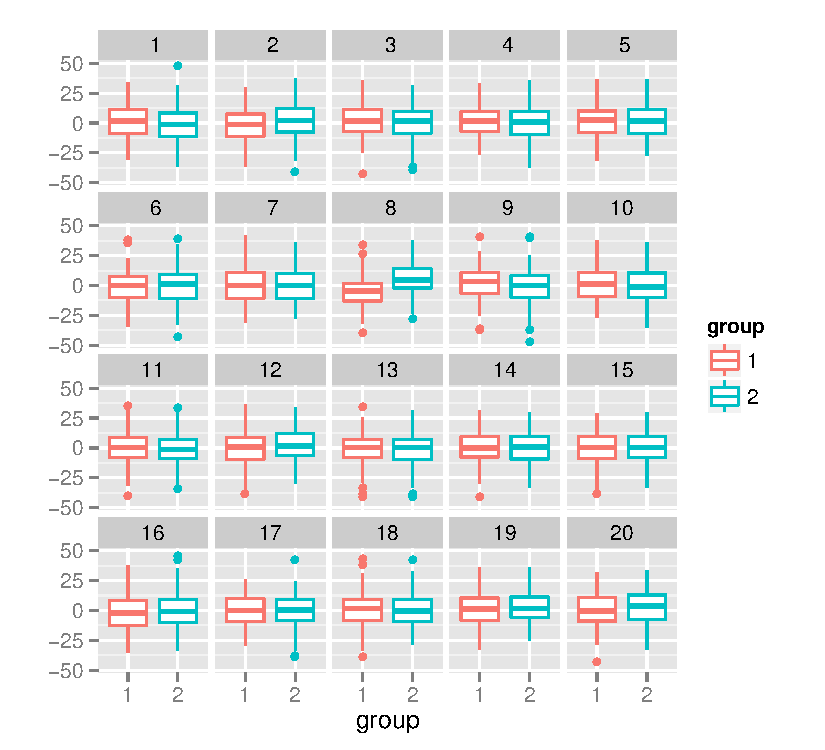
\includegraphics[width=.95\textwidth]{turk1-example.pdf}
% % plot_turk1_100_16_12_3
% %\includegraphics[width=.65\textwidth]{large-p-trim-bin.pdf}
% \caption{An example lineup from Turk Experiment 1. The lineup has $m = 20$ plots of which one is the observed data plot and the remaining $m - 1$ are the null plots generated assuming that the null hypothesis is true. Subjects were asked to identify the plot which has the largest vertical difference between the two groups. Can you identify the observed data plot?}
% \label{turk1}
% \end{figure}

For each lineup, the detection rate is calculated based on the number of evaluations and data identifications by subjects and related to its $\delta$-difference and $\gamma$-number of extreme null plots using both the distance based on boxplots ($d_{BX}$) and the binned distance ($d_{BN}$, using 8 bins in y direction and 2 in x).  
%\hh{XXX this needs some more work XXX}
%For each lineup a subject's choice was noted and the proportion of data identifications was calculated. The distances between the plots in each lineup were computed using both the distance based on boxplots ($d_{BX}$) and the binned distance ($d_{BN}$). For each lineup the mean distance for the true plot and the null plots were calculated and $\delta$ and $\gamma$ are obtained. The proportion of data identification is plotted against each of the two statistics, shown in Figure~\ref{turk1comp}. Binned distance was calculated using 8 bins \hh{along the $y$ axis$ and 2 for $x$}. %shows the detection rate against the difference for $d_{BX}$ and $d_{BN}$ and the number of null plots greater than the observed plot for the two distance measures. 


\begin{figure}[!t]
\centering
\begin{subfigure}[t]{\textwidth}
\centering
%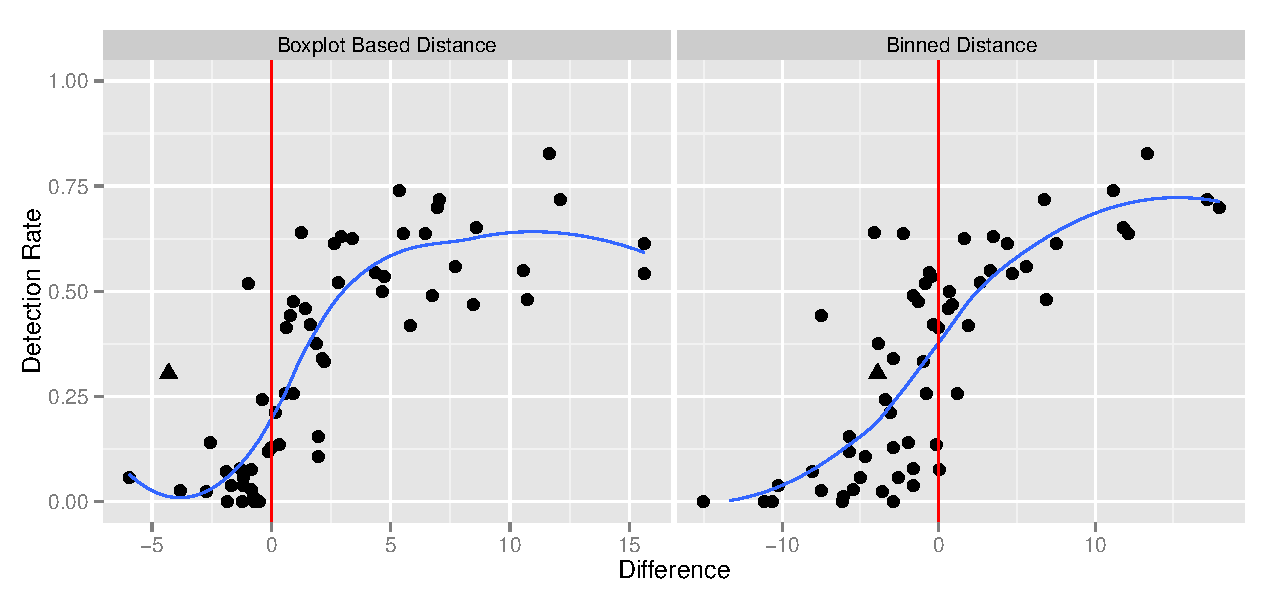
\includegraphics[width=\textwidth]{turk1-prop-box-bin.pdf}
\caption{\label{fig:turkcomp-1}Scatterplots of detection rate versus $\delta$-difference}
\begin{knitrout}
\definecolor{shadecolor}{rgb}{0.969, 0.969, 0.969}\color{fgcolor}
\includegraphics[width=0.7\textwidth]{figure/dist-box-bin-1} 

\end{knitrout}
\end{subfigure}
\begin{subfigure}[t]{\textwidth}
\centering
\caption{\label{fig:turk1comp-2}Scatterplots of detection rate versus $\gamma$-number of extreme nulls}
%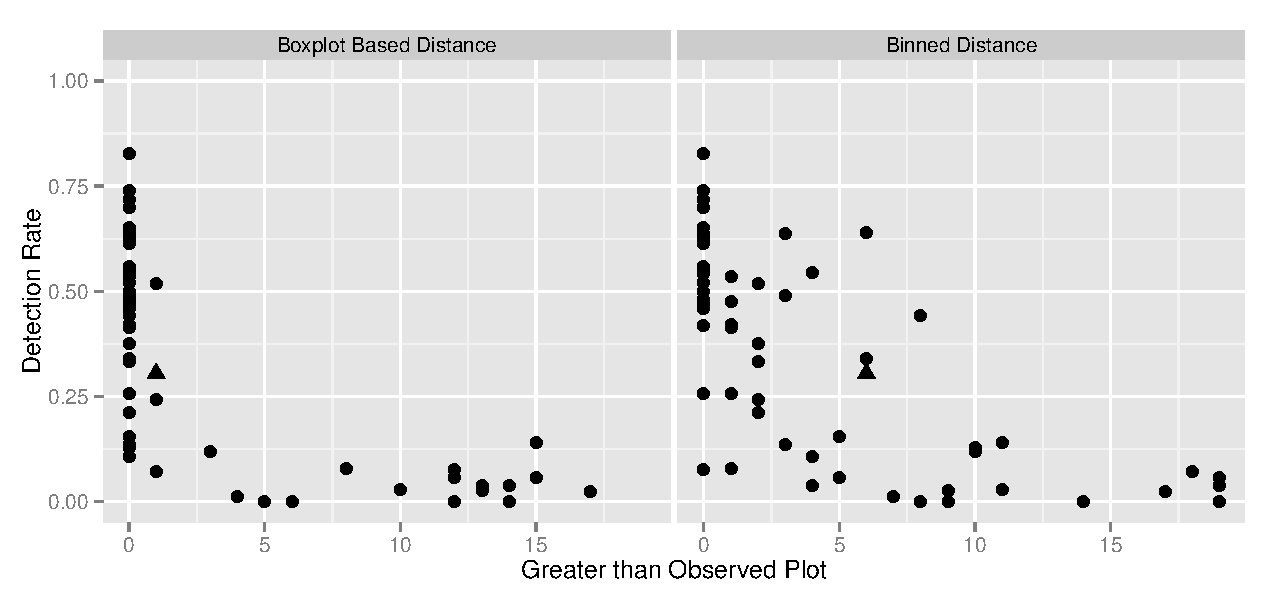
\includegraphics[width=0.7\textwidth]{turk1-grtr-box-bin.pdf}
\begin{knitrout}
\definecolor{shadecolor}{rgb}{0.969, 0.969, 0.969}\color{fgcolor}
\includegraphics[width=0.7\textwidth]{figure/gamma-turk1-1} 

\end{knitrout}
\end{subfigure}
	\vspace{-.1in}
\caption{Comparison of distance metrics for side-by-side boxplots. Detection Rate (a) and the number of plots greater than the observed (b) are plotted against the difference based on the boxplot and binned distance. The vertical line represents the difference equal to zero when there is at least one null plot similar to the observed plot. The detection rate increases with the difference. As the number of plots with distance greater than the observed increases, the detection rate decreases.  The triangle represents a lineup which has a high detection rate but a negative $\delta$-difference. This particular lineup is examined in Figure~\ref{turk1-exp}. }
\label{turk1comp}
%{Caption of subfigures \subref{fig:subfig1}, \subref{fig:subfig2} and \subref{fig:subfig3}}
\end{figure}

%\newpage
These values are plotted in Figure~\ref{turk1comp}.
We see that as $\delta$-difference increases, detection rate generally increases. The solid lines in Figure~\ref{fig:turkcomp-1} are fits  from  logistic regression models using a quadratic effect for distance.
The fitted lines come very close to the non-parametric smooth shown by the dashed line. Qualitatively, both boxplot based distance and binned distance show very similar fits for detection rate. Based on the logistic regressions, boxplot distance is fitting detection rate a bit better (AIC: 798.7) than binned distance  (AIC: 826). 

Figure~\ref{fig:turk1comp-2} shows the relationship between detection rate and the $\gamma$-number of extreme null plots. As this number increases, it gets harder for subjects to identify the data plot. It is interesting to see that for some lineups subjects are able to  pick the data plot even if there are  one or two more extreme null plots. 

Though  distance based on  boxplots works better a bit,  binned distance does a decent job in this case. According to the binned distance, there are a few lineups, in which  the data plot is identified in more than 60\% of all evaluations despite a negative $\delta$-difference (see also Figure~\ref{turk1comp}). It should be noted that the binned distance does not take any graphical elements of the plot (such as the box or whiskers) into account but calculates distance solely based on the data. So outliers may have an effect on the binned distance but might not affect the distance based on the boxplots. 

If participants base their choice on graphical elements, binned distance might therefore not be able to adequately reflect this.
In order to investigate on what participants base their choice, we are going to have a closer look at an individual lineup. 

From Figure~\ref{turk1comp} we see that for some of the lineups the detection rate is higher than its $\delta$-difference would suggest. One such lineup is marked using a triangle in Figure~\ref{turk1comp}. %It would be interesting to look into the lineup closely to identify what made the people pick the actual plot as different. 
Figure~\ref{turk1-exp} shows the lineup and the distribution of distance metrics for a closer look at what might observers lead to pick the data plot as different. The grey numbers at the bottom right of each of the plots in the lineup shows a summary of how often a plot was picked by a participant in 168 evaluations.

\begin{figure}[!p]
\centering
\begin{subfigure}[t]{\textwidth}
\centering
\caption{\label{fig:turk1-exp-1}Lineup of side-by-side boxplots. }
%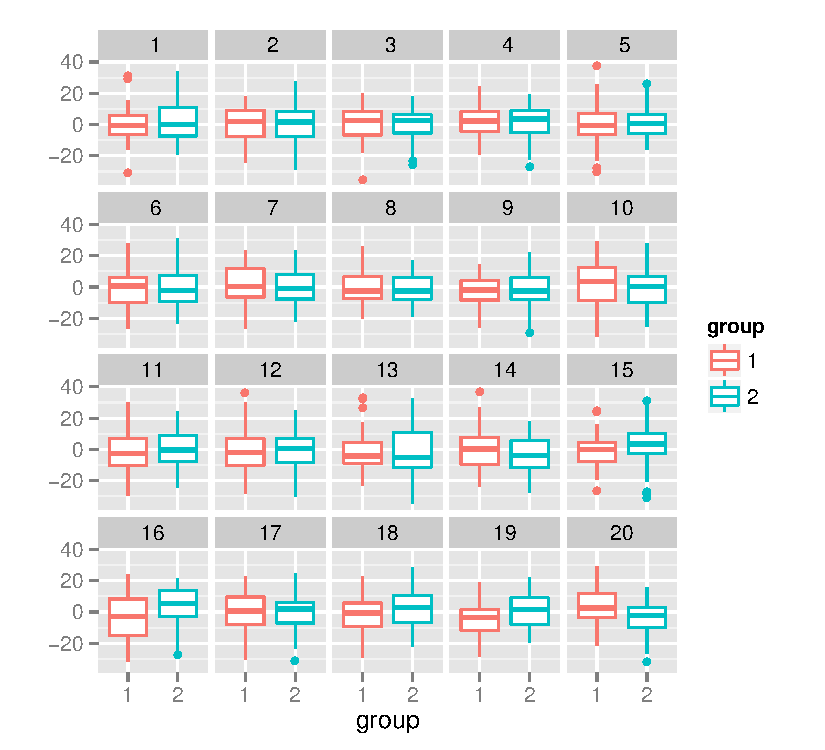
\includegraphics[width=\textwidth]{lineup-high-prop-neg-diff.pdf}
\begin{knitrout}
\definecolor{shadecolor}{rgb}{0.969, 0.969, 0.969}\color{fgcolor}
\includegraphics[width=0.6\textwidth]{figure/lp-exc-1} 

\end{knitrout}
\end{subfigure}\hfill




\begin{subfigure}[t]{0.32\textwidth}
%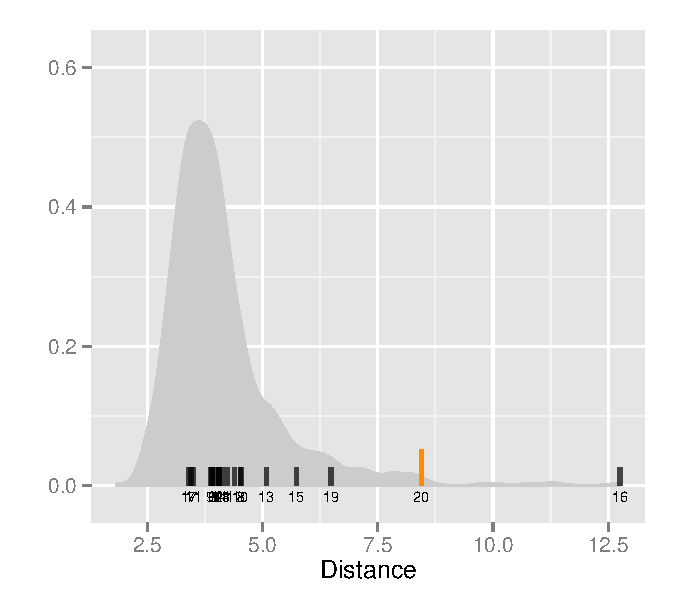
\includegraphics[width=\textwidth]{distribution-box-dist-exp1.pdf}
\caption{\small Boxplot based distance}
\begin{knitrout}
\definecolor{shadecolor}{rgb}{0.969, 0.969, 0.969}\color{fgcolor}
\includegraphics[width=\textwidth]{figure/dbx-1} 

\end{knitrout}
\end{subfigure}
\begin{subfigure}[t]{0.32\textwidth}
%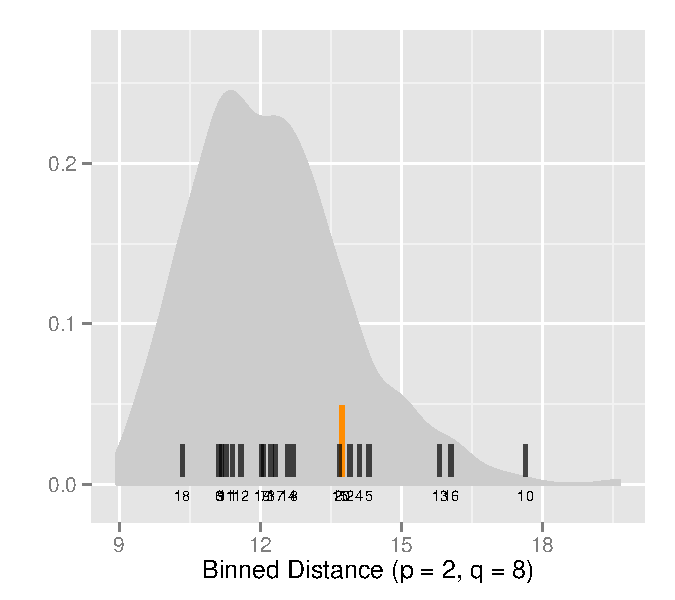
\includegraphics[width=\textwidth]{distribution-bin-dist-2-8-exp1.pdf}
\caption{\small Binned (2,8) distance}
\begin{knitrout}
\definecolor{shadecolor}{rgb}{0.969, 0.969, 0.969}\color{fgcolor}
\includegraphics[width=\textwidth]{figure/b28-1} 

\end{knitrout}
\end{subfigure}
\begin{subfigure}[t]{0.32\textwidth}
%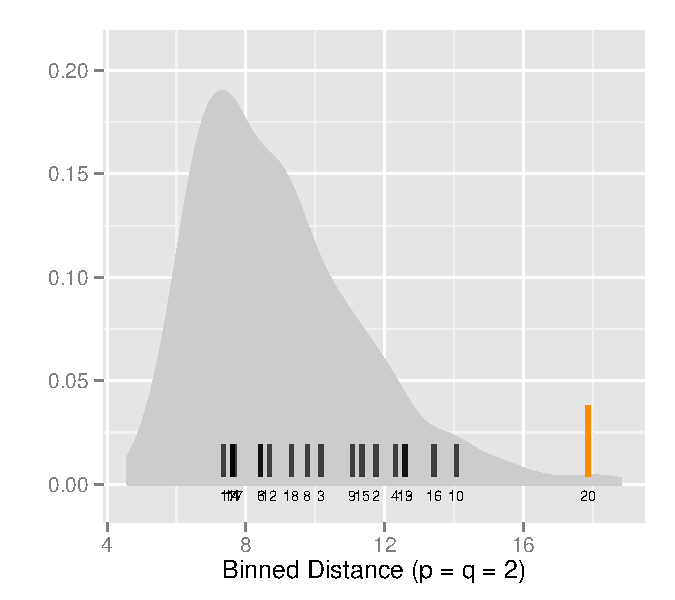
\includegraphics[width=\textwidth]{distribution-bin-dist-2-2-exp1.pdf}
\caption{\small Binned (2,2) distance}
\begin{knitrout}
\definecolor{shadecolor}{rgb}{0.969, 0.969, 0.969}\color{fgcolor}
\includegraphics[width=\textwidth]{figure/b22-1} 

\end{knitrout}
\end{subfigure}

	\vspace{-.1in}
\caption{Illustration of the behavior of the three distance metrics. The lineup is shown in (a) and  distributions of the different  metrics based on this lineup is shown in the other plots: boxplot based distance in (b), binned distance with 2 and 8 bins on x and y axis in (c) and binned distance with 2 bins along both axes in (d). Grey numbers on the lineup show the counts of subject choices. The lineup corresponds to the point marked with a triangle in difference vs. detection rate plot in Figure~\ref{turk1comp}. }
\label{turk1-exp}
%{Caption of subfigures \subref{fig:subfig1}, \subref{fig:subfig2} and \subref{fig:subfig3}}
\end{figure}
%\afterpage{\clearpage}

%The lineup in Figure~\ref{turk1-exp} is a lineup of side-by-side boxplots.
The observed data plot is Plot \#20, which has been picked most often by participants, but there are other plots that are being chosen quite frequently. Plot \#16 is the plot with the  largest boxplot distance. This is reflected by the large number of times this plot has been singled out by observers. 

Maybe surprisingly, plots Plots \#19 and \#15, which have relatively large differences between the quartiles, are not being chosen by many participants. Instead, observers seem to focus on the difference in interquartile ranges (i.e.\ the height of the box in a  boxplot). Plots \#1, \#13 and \#16 exhibit a large interquartile difference and are being picked often by observers.


The time subjects  take to respond to a lineup is another measure that can be used to evaluate their difficulty. 
Due to the presence of some huge outliers, we decided to use the median of time taken for each lineup. These values are plotted against  $\delta$-difference for both distance measures as shown in Figure~\ref{turk1-mtime}.
Both $\delta$-difference exhibit a similar pattern: the time to respond peaks at a $\delta$-difference of zero. This indicates, that the situation where two or more plots exhibits similarly extreme features is the most difficult for observers to judge. With negative $\delta$-differences at least one null plot is more extreme, and observers seem to be able to make their choice quickly (probably for the extreme null plot).
%It can be clearly seen that when $\delta$-difference is below 0, there is no real trend in the mean time and there is a huge variability, indicating that the time taken depends on the subjects.
%\hh{XXX variability doesn't change that much over $x$; XXX for boxplot based distance the time to respond peaks at a $\delta$-difference of zero. This might indicate, that this situation is the most difficult for observers to judge. When there are more extreme plots, observers seem to be able to make their choice quickly (probably for the extreme null plot).}
When $\delta$-difference is positive, the median time to respond decreases rapidly as $\delta$-difference increases. Hence, subjects are able to make their choice of a plot more quickly if the true plot is extreme compared to the null plots.

Note that taking the log of time to respond is an alternative to using the median. Qualitatively, the relationships to distance metrics are very similar for median and log time taken, but median time is much easier to interpret. 

% \hh{XXX I don't think that the following statement is true -- there is no reason, why boxplot distance and binned distance should be on the same scale. }
% For Turk 1 experiment, the value of the ratio for boxplot distance is 86.52 and for binned distance is 18.82. This indicates that the boxplot distance works better than the binned distance. 
 
%\begin{figure}[hbtp]
%\centering
%\subfigure[]{
%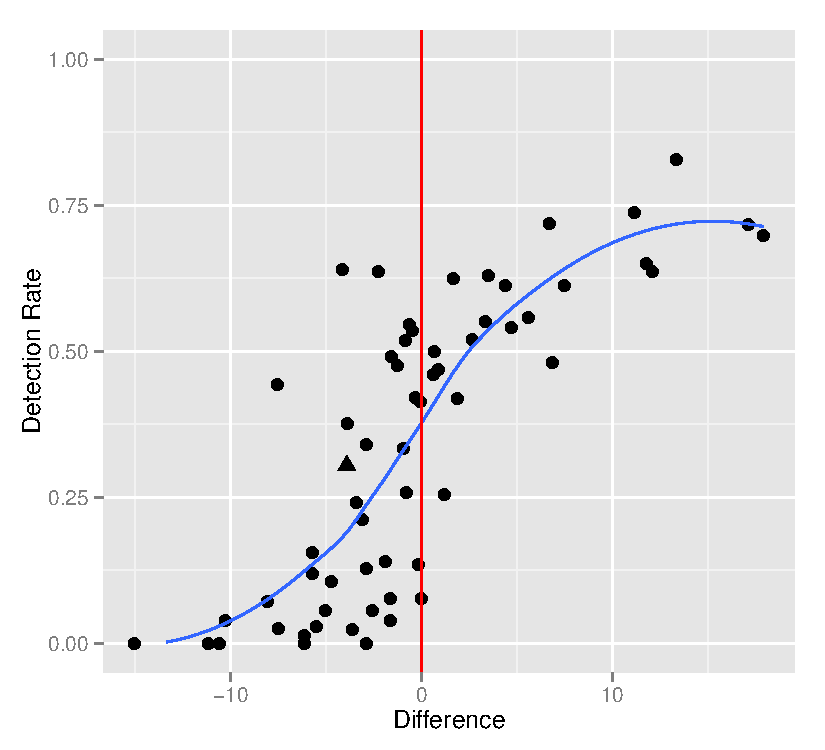
\includegraphics[scale=0.55]{turk1-diff-bin-prop-8.pdf}
%\label{t1bin_1}
%}
%\subfigure[]{
%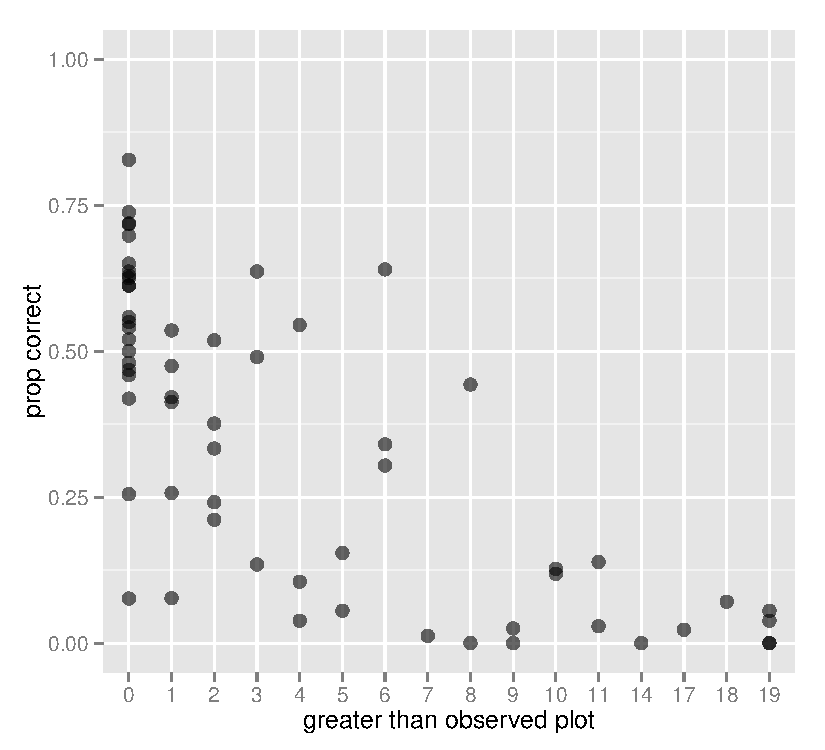
\includegraphics[scale=0.55]{turk1-grtr-bin-prop-8.pdf}
%\label{t1bin_2}
%}
%%\label{turk1-bin}
%	\vspace{-.1in}
%\caption{(a) Plot showing the proportion correct against the difference based on the binned distance with 8 bins on each axis. The vertical line represents the difference equal to 0 when there is at least one null plot similar to the observed plot. The proportion correct increases with the difference. (b) Plot showing the proportion correct against the number of null plots greater than the observed plot according to the binned distance. The proportion correct decreases as the number of null plots greater than the observed plot increases.  }
%%{Caption of subfigures \subref{fig:subfig1}, \subref{fig:subfig2} and \subref{fig:subfig3}}
%\end{figure}

\begin{figure}[!h]
\centering
%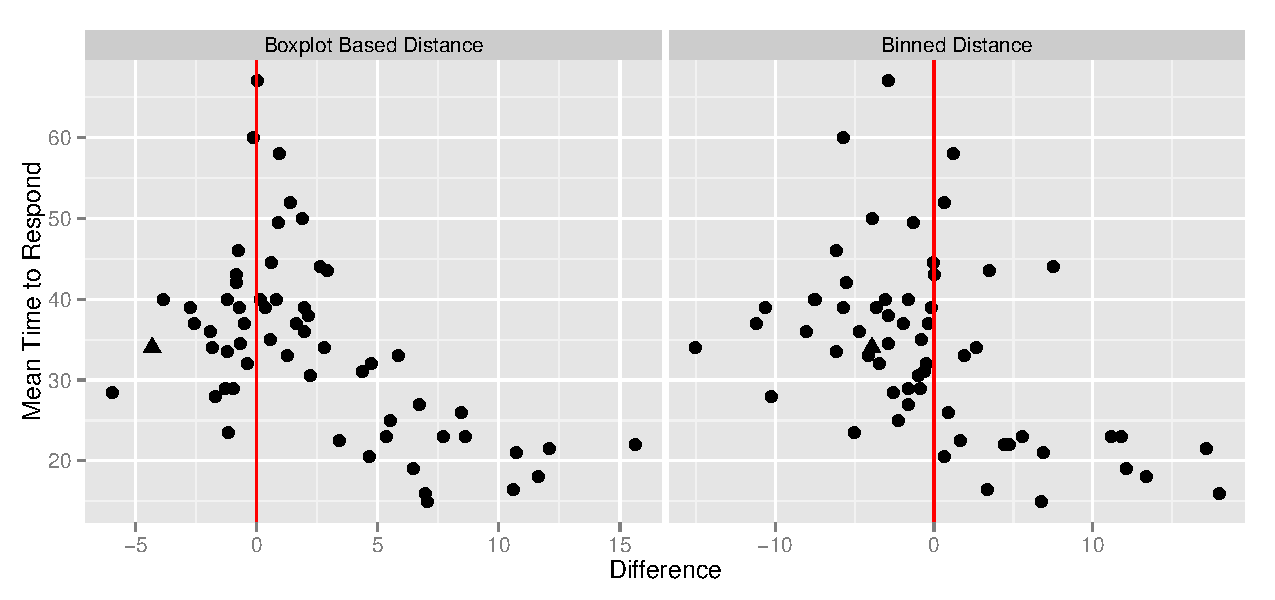
\includegraphics[width=0.6\textwidth]{turk1-mtime-box-bin.pdf}
\begin{knitrout}
\definecolor{shadecolor}{rgb}{0.969, 0.969, 0.969}\color{fgcolor}
\includegraphics[width=0.6\textwidth]{figure/time-taken-1} 

\end{knitrout}
%\subfigure[]{
%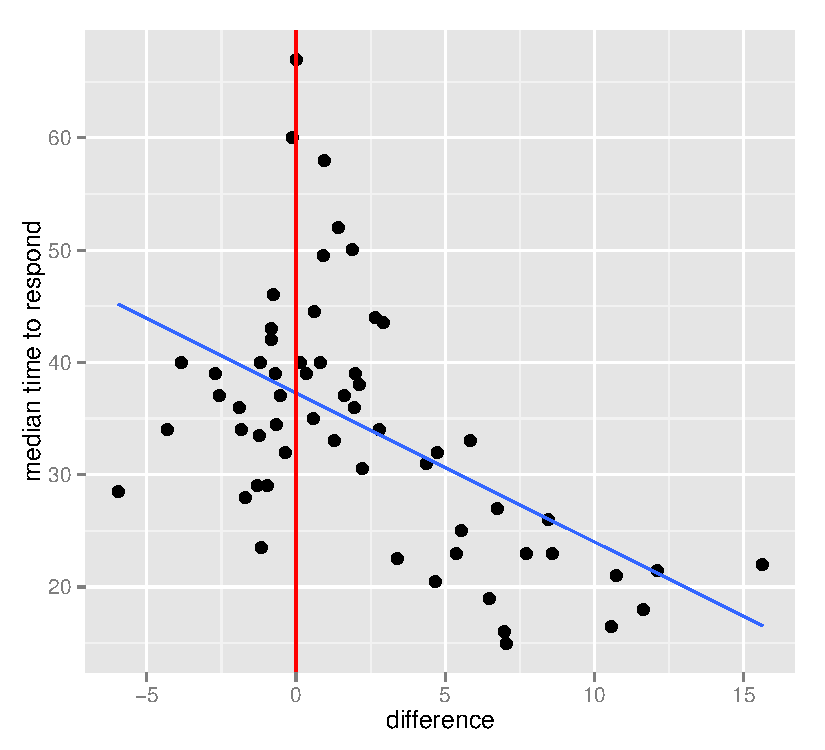
\includegraphics[scale=0.55]{turk1-diff-box-mtime.pdf}
%\label{t1comp_1}
%}
%\subfigure[]{
%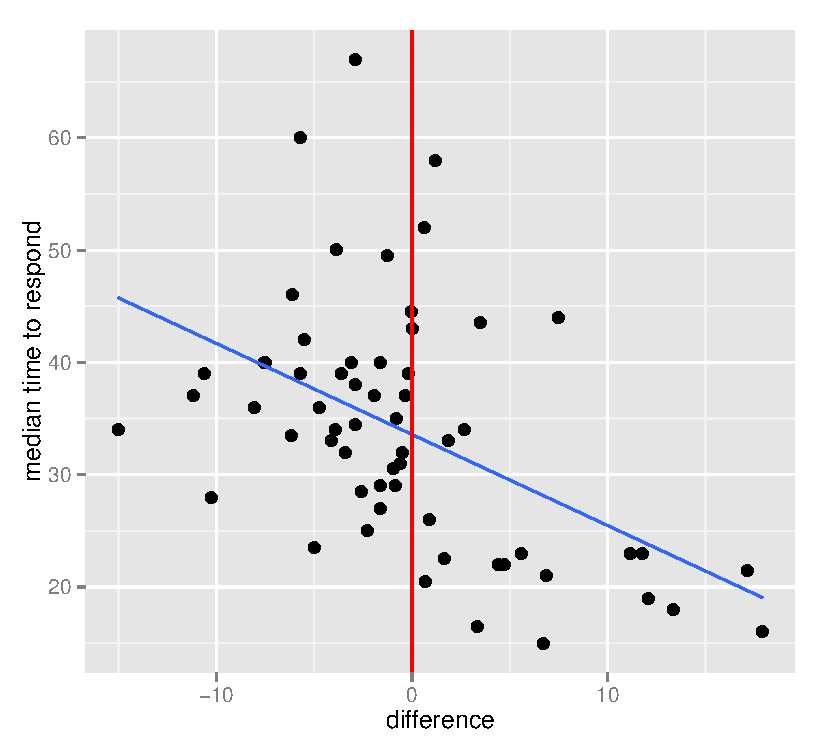
\includegraphics[scale=0.55]{turk1-diff-bin-mtime.pdf}
%\label{t1bin_1}
%}
	\vspace{-.1in}
\caption{Comparison of distance metrics for side-by-side boxplots. Median time to respond is plotted against $\delta$-difference based on boxplot and binned(2,8) distance. The vertical line represents a $\delta$-difference equal to zero when there is at least one null plot similar to the observed plot. Median time to respond decreases as $\delta$-difference increases. The triangle marks again the lineup examined in detail in Figure~\ref{turk1-exp}. }
\label{turk1-mtime}
%{Caption of subfigures \subref{fig:subfig1}, \subref{fig:subfig2} and \subref{fig:subfig3}}
\end{figure}


%\newpage
\subsection{Experiment II -- Scatterplots with an Overlaid Regression Line}\label{sec:turk2}
The question of interest of experiment II is very similar to the one in experiment I: again, the focus is to investigate the power of visual methods in the framework of normal models. In contrast to experiment I, we are interested in the significance of a continuous variable $X$. The test statistic therefore is a scatterplot of the dependent variable and $X$ overlaid by a regression line. As mentioned in the introduction and further discussed in section 5.2 of \citet{majumder:2011}, $X$ is assumed to be standard normal, and dependent data $Y$ is also simulated from a normal distribution for various correlation settings. Null data correspondingly is simulated from $N(X\widehat{\beta}, \widehat{\sigma}^2)$.  
Figures~\ref{lineup-example} and~\ref{fig:distances} show examples of the type of  lineup used in the study.  Subjects recruited from MTurk  were shown a set of ten lineups  and asked to identify the plot with the steepest slope in each. 

For each lineup in this experiment,  distances between the plots were computed using both  regression based distance  ($d_{RG}$) and  binned distances ($d_{BN}$) with a small number of bins. For each lineup the proportion of data identifications was calculated from participants' responses and plotted against $\delta$-difference and the $\gamma$-number of extreme null plots, as shown in Figure~\ref{turk2comp}.

\begin{figure}[!t]
\begin{subfigure}[t]{\textwidth}
\centering
\caption{\label{turk2comp-1}$\delta$-difference }
%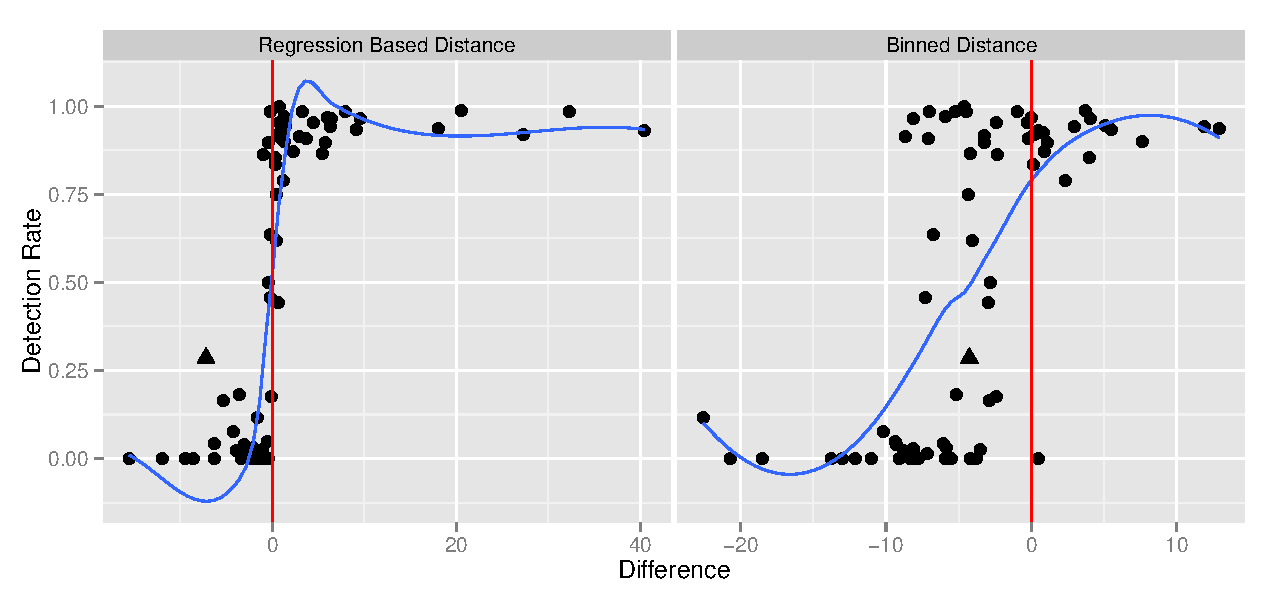
\includegraphics[width=0.7\textwidth]{turk2-prop-reg-bin.pdf}
\begin{knitrout}
\definecolor{shadecolor}{rgb}{0.969, 0.969, 0.969}\color{fgcolor}
\includegraphics[width=0.7\textwidth]{figure/delta-turk2-1} 

\end{knitrout}
\end{subfigure}
\begin{subfigure}[t]{\textwidth}
\centering
\caption{\label{turk2comp-2}$\gamma$-number of extreme nulls }
%\includegraphics[width=0.7\textwidth]{turk2-grtr-reg-bin.pdf}
\begin{knitrout}
\definecolor{shadecolor}{rgb}{0.969, 0.969, 0.969}\color{fgcolor}
\includegraphics[width=0.7\textwidth]{figure/gamma-turk2-1} 

\end{knitrout}
\end{subfigure}
%\subfigure[]{
%\includegraphics[scale=0.55]{turk2-grtr-reg-prop.pdf}
%\label{t2comp_1}
%}
%\subfigure[]{
%\includegraphics[scale=0.55]{turk2-grtr-bin-prop-2.pdf}
%\label{t2comp_2}
%}
	\vspace{-.1in}
\caption{Comparison of distance metrics for scatterplots with a regression line overlaid.  Detection rate is plotted against (a) $\delta$-difference  and (b) $\gamma$-number of extreme null plots  based on  regression and binned distances. The vertical line represents the difference equal to zero when there is at least one null plot with an identical difference measure to the data plot. 
Detection rate increases  on average with $\delta$-difference. As the $\gamma$-number of extreme null plots increases,  detection rate decreases.  The triangle represents a lineup which has high detection rate but negative difference. This particular lineup is examined in Figure~\ref{turk2-exp}.}
\label{turk2comp}
%{Caption of subfigures \subref{fig:subfig1}, \subref{fig:subfig2} and \subref{fig:subfig3}}
\end{figure}
%\afterpage{\clearpage}

%Figure~\ref{turk2comp-1} shows a scatterplot of detection rate against $\delta$-difference. 
 As $\delta$-difference increases,  average detection rate increases, i.e.\ subjects do better in  easier lineups than hard ones. The solid lines show fits of logistic regressions of detection rate in $\delta$-difference based on regression (AIC: 746.9) and based on binned distance (AIC: 2150.7). Both fits come reasonably close to the dashed lines of a non-parametric loess smooth, indicating that they explain most of the relationship between $\delta$-difference and detection rate.
The regression based distance works well in capturing the complexity of the lineups. %The difference is positive for lineups with large differences and negative for lineups with small difference. 
A few lineups have a $\delta$-difference close to zero, marked by the vertical line -- for those lineups detection rates of lineups flip from being close to zero to close to one within a very short interval. 

For binned distance the situation is quite different.  Although detection rate increases with difference, the detection rate is already quite high for lineups with negative differences. This is a classic scenario where the distance does not capture all the features on which observers base their choice: here, a graphical element --the line-- affects the response, and shifts detection rates horizontally. %The presence of the overlaid regression line on almost transparent points of the scatterplot affects the response of the subjects. 
%Another reason may be the use of the same number of bins (2 $\times$ 2) in this case for all the lineups. The relationship may improve if different number of bins would be used for different lineups.
While this makes an absolute comparison of distances across different types of plots impossible, we can still use binned distance as a relative measure to judge difficulty.


Figure~\ref{turk2comp-2} shows  detection rate against the $\gamma$-number of extreme null plots. As the number of extreme plots increases,  detection rate decreases on average --- indicating that identifying the data plot from a lineup becomes harder when there are more extreme plots in the lineup. For a few lineups, almost all evaluations led to an identification of the data plot although there was one null plot with an extreme feature. From Figure~\ref{turk2comp-1}, we see that this difference is marginal in most cases, though. 

\begin{figure}[!t]
\centering
%\includegraphics[scale=0.75]{turk2-mtime-reg-bin.pdf}
%\subfigure[]{
%\includegraphics[scale=0.55]{turk2-diff-reg-mtime.pdf}
%\label{t1comp_1}
%}
%\subfigure[]{
%\includegraphics[scale=0.55]{turk2-diff-bin-mtime.pdf}
%\label{t1bin_1}
%}
\begin{knitrout}
\definecolor{shadecolor}{rgb}{0.969, 0.969, 0.969}\color{fgcolor}
\includegraphics[width=0.75\textwidth]{figure/turk2-time-1} 

\end{knitrout}
	\vspace{-.1in}
\caption{Comparison of distance metrics for scatterplots with a regression line over laid. Median time to respond is plotted against $\delta$-difference based on  regression based and binned(2,2) distance. The vertical line represents a $\delta$-difference equal to zero, i.e.\ there is at least one null plot similar to the observed plot. The median time to response decreases as $\delta$-difference increases. The triangle represents a lineup which is examined in Figure~\ref{turk2-exp}.   }
%{Caption of subfigures \subref{fig:subfig1}, \subref{fig:subfig2} and \subref{fig:subfig3}}
\label{turk2-mtime}
\end{figure}
%%\afterpage{\clearpage}

Figure~\ref{turk2-mtime} shows the relationship between the median time taken to respond and $\delta$-difference for both the distances. It can be clearly seen that there is a strong negative association: as $\delta$-difference increases, the subjects take less time to respond. Similar to the previous example of section~\ref{sec:turk1} time to respond peaks at a $\delta$-difference close to zero.
%In the case of the binned distance, the relationship is negative though the variability is higher for the above mentioned reasons.

Although the regression based distance seems to efficiently identify the quality of the lineup, there is one lineup (marked by a solid triangle in Figure~\ref{turk2comp}) with a negative $\delta$-difference which was nevertheless identified by observers reasonably successfully.  Figure~\ref{turk2-exp} shows the lineup and the corresponding distributions of distance metrics. 








\begin{figure}[!p]
\centering
\begin{subfigure}[b]{\textwidth}
\caption{\small Lineup of scatterplots with overlaid regression lines.}
\centering
\begin{subfigure}[b]{0.6\textwidth}
%\includegraphics[width=\textwidth]{lineup-exp2-neg-diff-large-prop.pdf}
\begin{knitrout}
\definecolor{shadecolor}{rgb}{0.969, 0.969, 0.969}\color{fgcolor}
\includegraphics[width=\textwidth]{figure/lp-turk2-exc-lp-1} 

\end{knitrout}
\end{subfigure}
%\hfill%\vfill
\begin{subfigure}[b]{0.3\textwidth}
\caption{Regression based distance}
\vspace{-.1in}
%\includegraphics[width=\textwidth]{distribution-reg-dist-exp2.pdf}
\begin{knitrout}
\definecolor{shadecolor}{rgb}{0.969, 0.969, 0.969}\color{fgcolor}
\includegraphics[width=\textwidth]{figure/unnamed-chunk-1-1} 

\end{knitrout}
\end{subfigure}
\end{subfigure}

\vspace{-.3in}
\begin{subfigure}[t]{0.3\textwidth}
\caption{Binned (2,2) distance}
\vspace{-.1in}
%\includegraphics[width=\textwidth]{distribution-bin-dist-2-2-exp2.pdf}
\begin{knitrout}
\definecolor{shadecolor}{rgb}{0.969, 0.969, 0.969}\color{fgcolor}
\includegraphics[width=\textwidth]{figure/unnamed-chunk-2-1} 

\end{knitrout}
\end{subfigure}
\begin{subfigure}[t]{0.3\textwidth}
\caption{Binned (8,2) distance}
\vspace{-.1in}
%\includegraphics[width=\textwidth]{distribution-bin-dist-8-2-exp2.pdf}
\begin{knitrout}
\definecolor{shadecolor}{rgb}{0.969, 0.969, 0.969}\color{fgcolor}
\includegraphics[width=\textwidth]{figure/unnamed-chunk-3-1} 

\end{knitrout}
\end{subfigure}
\begin{subfigure}[t]{0.3\textwidth}
\caption{$p$-values}
\vspace{-.1in}
%\includegraphics[width=\textwidth]{distribution-pval-exp2.pdf}
\begin{knitrout}
\definecolor{shadecolor}{rgb}{0.969, 0.969, 0.969}\color{fgcolor}
\includegraphics[width=\textwidth]{figure/unnamed-chunk-4-1} 

\end{knitrout}
\end{subfigure}

\caption{Illustration of the behavior of different distance metrics. The lineup is shown in (a) and the distributions of different distance metrics using this lineup are shown in plots (b)--(d): regression based distances in (b), binned distance with 2 bins on each axes in (c), and binned distance with 8 and 2 bins in x and y axis (d). In (e), the distribution of the conventional $p$-values are plotted with $p$-values for the lineups marked on the distribution. Grey numbers on the lineup show the counts of subject choices. The lineup corresponds to the point marked with a triangle in difference vs. detection rate plot in Figure~\ref{turk2comp}.}
\label{turk2-exp}
%{Caption of subfigures \subref{fig:subfig1}, \subref{fig:subfig2} and \subref{fig:subfig3}}
\end{figure}
%\afterpage{\clearpage}

The lineup in Figure~\ref{turk2-exp} is a difficult one as suggested by the distribution of the distance metrics based on regression. 
For the data plot (in panel \#10) the conventional $p$-value for testing the slope equal to zero is 0.085. However, the signal in the plot is strong enough, to make  around 28\% of all subjects pick this plot.

The binned distance with 2 bins on each axes does not let the data plot stand out in any way, however, the binned distance using the optimal number of bins (8 on the x-axis and 2 on the y-axis) by the optimal number of bins selection method identifies the data plot as different from the others. 

The number of picks lines up best with the difference measure based on the slope (regression without intercept). Plots \#10, 12, 11, 9, and 7 all have a relatively steep slope, and are also the plots that were picked the most often.  
Again, a distance measure derived directly from one of the graphical elements in the plot leads to the best assessment of the choices made by human evaluators.


\subsection{Experiment III -- Large $p$, Small $n$ Data}

The motivation behind this experiment is to study the effect of high dimensions on separability in data. Scenarios with pure noise and some real separation in two or three groups were investigated. %Data was simulated with different dimensions and fixed sample size. Data was divided into two or three groups. 
A projection pursuit with Penalized Discriminant Analysis Index \citep{lee:2009} was used to obtain one (for two groups) or two (for three groups) dimensional projections. 
Depending on the number of groups, either a jittered dotplot or a scatterplot was used as test statistic in a lineup setting. %The one or two dimensional projections were then plotted which resulted in the observed data plot. 
The null plots are obtained by permuting the group variable and plotting the two dimensional projections obtained from a projection pursuit with PDA index.
The subjects were shown these lineups and were asked to identify the plot with the most separated colored groups. %Figure~\ref{largep} gives an example of such a lineup of a  two dimensional projection with three colored groups. 

%\begin{figure}[!t]
%\centering
%\includegraphics[width=.95\textwidth]{largep-example.pdf}
%\includegraphics[width=.65\textwidth]{large-p-trim-bin.pdf}
%<<t7-lp, echo=FALSE, fig.width=6, fig.height=6, out.width='.7\\textwidth'>>=
%lpt7 <- read.table("data/turk7/dat_large_p_small_n_30_20_0_2_1.txt", header=TRUE)

%qplot(X1, X2, colour=factor(cl), facets=~.sample, data=lpt7, size=I(3)) + 
%  theme_lineup +
%  theme(legend.position="none") 
%@
%\caption{An example lineup from Experiment III. Here, two dimensional projections of the PDA index are plotted for $n = 30$ observations in 20 dimensional data with separation. The subjects were asked to identify the plot with the most separated colors. Can you identify the data plot?}
%\label{largep}
%\end{figure}
%%\afterpage{\clearpage}

The distances between the plots in this experiment were computed using the distance based on minimum separation and average separation of the clusters and also the binned distance. The number of bins used for the lineups with one dimensional projections is larger (10 in this case) but for the lineups with two dimensional projections, the number of bins used is 5. The proportion of correct response is plotted against $\delta$-difference and $\gamma$-number of extreme nulls for both distances. Figure~\ref{lp-comp} shows the results.






\begin{figure}[!t]
\centering
\begin{subfigure}[t]{\textwidth}
\caption{$\delta$-difference}
\centering
%\includegraphics[width=\textwidth]{largep-prop-sep-bin.pdf}
\begin{knitrout}
\definecolor{shadecolor}{rgb}{0.969, 0.969, 0.969}\color{fgcolor}
\includegraphics[width=\textwidth]{figure/largep-delta-1} 

\end{knitrout}
\end{subfigure}
\begin{subfigure}[t]{\textwidth}
\caption{$\gamma$-number of extreme null plots}
\centering
%\includegraphics[width=\textwidth]{largep-grtr-sep-bin.pdf}
\begin{knitrout}
\definecolor{shadecolor}{rgb}{0.969, 0.969, 0.969}\color{fgcolor}
\includegraphics[width=\textwidth]{figure/largep-gamma-1} 

\end{knitrout}
\end{subfigure}

	\vspace{-.1in}
\caption{Comparison of distance metrics for the scatterplot with clusters. Detection rate is plotted against (a) $\delta$-difference and (b) against $\gamma$-number of extreme nulls, using distances based on minimum separation, average separation, binned and Dunn's distance. The vertical line represents the difference equal to zero when there is at least one null plot similar to the observed plot. Solid blue line represents the fitted logistic regression model and the dashed blue line shows a loess smoother.  Detection rate generally increases with $\delta$-difference. As the $\gamma$-number of extreme null plots increases, detection rate decreases. The triangle represents a lineup with high detection rate and negative difference based on the average separation distance. This is examined in Figure~\ref{lp-exp}. }
\label{lp-comp}
%{Caption of subfigures \subref{fig:subfig1}, \subref{fig:subfig2} and \subref{fig:subfig3}}
\end{figure}
%%\afterpage{\clearpage}

In Figure~\ref{lp-comp}, the detection rate is plotted against the difference for distance based on minimum separation, average separation and the binned distance. The  vertical line shows a difference equal to zero.  It can be seen that as the difference increases, the detection rate increases and all distances do a reasonably good job in capturing the response of the subjects. In terms of the logistic regression fit to the data, average separation is a bit ahead according to AIC (AIC: 349.6) 
compared to minimal separation  (AIC: 422.8) 
and binned distance (AIC: 543.4). Dunn separation, motivated from cognitive perception, comes in at a maybe surprising last place (AIC: 697.3).

In (b) it can be seen that as there are more extreme null plots compared to the observed plot, the subjects find it difficult to pick the observed plot. For a few lineups, a large number of the subjects identify the observed plot although there is more extreme null plots. 

\begin{figure}[!h]
\centering
%\includegraphics[width=0.7\textwidth]{largep-mtime-sep-bin.pdf}
\begin{knitrout}
\definecolor{shadecolor}{rgb}{0.969, 0.969, 0.969}\color{fgcolor}
\includegraphics[width=\textwidth]{figure/largep-mtime-1} 

\end{knitrout}

	\vspace{-.1in}
\caption{Plot showing the median time to respond by the subjects against the difference based on the minimum separation distance, average separation and binned distance. The vertical line represents the difference equal to 0 when there is at least one null plot similar to the observed plot. The median time decreases as the difference increases.  }
\label{lp-mtime}
%{Caption of subfigures \subref{fig:subfig1}, \subref{fig:subfig2} and \subref{fig:subfig3}}
\end{figure}
%\afterpage{\clearpage}

Figure~\ref{lp-mtime} shows the relationship between the median time observers take to respond  and $\delta$-difference for the three different distances. It can be clearly seen that there is a strong negative association; as the difference increases,  subjects take less time to respond. %Also the variability of the mean time is higher for smaller difference. In case of binned distance, the relationship is negative though the variability is higher for all differences.
For both average separation and binned distance we see a peak in response time, i.e.\ for large negative $\delta$-difference the median time to respond decreases again.




\begin{figure}[!p]

%\centering
\begin{subfigure}[t]{\textwidth}
%\centering
\caption{Lineup of scatterplots of three groups. Which plot shows the best separation? \hfill}
\centering
\begin{subfigure}[b]{0.6\textwidth}
%\includegraphics[width=\textwidth]{lineup-large-p-small-n.pdf}
\begin{knitrout}
\definecolor{shadecolor}{rgb}{0.969, 0.969, 0.969}\color{fgcolor}
\includegraphics[width=\textwidth]{figure/lp-exc-t7-1} 

\end{knitrout}
\end{subfigure}
%\hfill%\vfill
\begin{subfigure}[b]{0.3\textwidth}
\caption{Binned (5,5) Distance}
%\includegraphics[width=\textwidth]{distribution-bin-dist-6-4-lpexp.pdf}
\begin{knitrout}
\definecolor{shadecolor}{rgb}{0.969, 0.969, 0.969}\color{fgcolor}
\includegraphics[width=\textwidth]{figure/bin55-1} 

\end{knitrout}
\end{subfigure}
\end{subfigure}%\hfill

\begin{subfigure}[t]{\textwidth} 
\centering
\begin{subfigure}[t]{0.3\textwidth}
\caption{Minimum Separation}
%\includegraphics[width=\textwidth]{distribution-min-sep-dist-lpexp.pdf}
\begin{knitrout}
\definecolor{shadecolor}{rgb}{0.969, 0.969, 0.969}\color{fgcolor}
\includegraphics[width=\textwidth]{figure/min_sep-1} 

\end{knitrout}
\end{subfigure} 
\begin{subfigure}[t]{0.3\textwidth}
\caption{Average Separation}
%\includegraphics[width=\textwidth]{distribution-ave-sep-dist-lpexp.pdf}
\begin{knitrout}
\definecolor{shadecolor}{rgb}{0.969, 0.969, 0.969}\color{fgcolor}
\includegraphics[width=\textwidth]{figure/avg_sep-1} 

\end{knitrout}
\end{subfigure} 
\begin{subfigure}[t]{0.3\textwidth}
\caption{Dunn Separation}
\begin{knitrout}
\definecolor{shadecolor}{rgb}{0.969, 0.969, 0.969}\color{fgcolor}
\includegraphics[width=\textwidth]{figure/dunn_sep-1} 

\end{knitrout}
\end{subfigure} 
\end{subfigure}
	\vspace{-.1in}
\caption{Illustration of the behavior of different distance metrics. The lineup is shown in (a) and the distributions of different distance metrics are shown in the other plots:  binned distance with 6 and 4 bins in x and y axis respectively in (b), distance based on minimum separation in (c), distance based on average separation in (d) and distance based on Dunn separation in (e). Grey numbers on the lineup show the counts of subject choices. The reference distributions are based on 100 null sets of 19 nulls each, yielding 1,800 distances.}
\label{lp-exp}
%{Caption of subfigures \subref{fig:subfig1}, \subref{fig:subfig2} and \subref{fig:subfig3}}
\end{figure}
%\afterpage{\clearpage}

Figure~\ref{lp-exp} shows the lineup in a high dimension, low sample size setting. The number of dimensions used is 100 and two of the dimensions have some separation. Plot \#20 shows the two-dimensional projections of the original data. This plot is, indeed, chosen in 13 out of 19 evaluations.  As the true plot does have real separation, it is to be expected that  subjects would be able to identify the plot. The distance based on average separation yields a negative difference showing that the lineup is difficult, while the distance based on minimum separation yields a positive difference. The distance metrics identify different characteristics in a plot. The average separation looks at the average of the distances of the points in a cluster to the points in other clusters.  Dunn separation performs very well in this example and correctly identifies the data panel as the panel with the strongest signal. While the binned distance shows plot \#20 as the one with the largest distance, this should be taken with care, because binned distance is, unlike the other two distances, not rotation invariant. In the case of plot \#20 the large distance merely indicates the difference in the arrangement of the clusters rather than their separation.


\section{Conclusion}
Distance metrics are compared to the response of human subjects on lineups. What we see in each of the experiments is that the general approach of the binned distance, while mostly performing decently, is usually out-done by a distance that is more tailored to the question of interest or takes the graphical elements into account. These data derived from a special collection of experiments where the task was very focused, but when the lineup is used in practice the question will be generic and we would expect the binned distance to be most broadly applicable. 

Different distance metrics better matched subjects' choices for the different plot types. Boxplot distance better matched subject choices in experiment I. Regression based distance matched better than binned distance for the subject choices in experiment II. By the $\gamma$-number, minimum separation and average separation matched subjects' choices better than the other distance metrics for experiment III. 
None of the distance metrics perfectly matches subject choices. This suggests that there is a lot of scope for exploring new ways to numerically characterize structure in plots. The metrics we have described were all based on the data, rather than the graphical elements in the plot. Utilizing the graphical elements, e.g. length of line relative the plot size to build metrics might provide a closer fit, and also help to understand more precisely what viewers are visually responding to in the plot. The lineup protocol provides a rigorous way to assess metrics on data plots with human vision. The examination of subject choices with metrics as done here provides a guide for assessing metrics systematically.

One of the purposes for developing the distance metrics discussed in this paper was to help in future experiments designed to assess visual inference with lineups. Being able to roughly divide lineups into three groups -- easy, moderate, difficult -- is useful for compiling blocks for subjects to evaluate. Subjects are typically given a block of ten lineups to evaluate. If all ten are difficult it is possible to frustrate the observer, and having ten easy lineups doesn't effectively harness the human resources. being able to roughy grade a lineup into these categories makes it easier  provide a reasonable set for each subject.  It is clear from this study that they are good for this rough categorization. 

%What the lineup protocol opens up to us is an approach that delivers us some objective insight into what people respond to in a plot and which graphical elements they consider when viewing a plot.


%While there is a fairly strong amount of agreement in most situations,  in some situations  they disagree. There does not seem to be one single reason behind this disagreement. Observers might identify a plot as different from the others in a lineup because of multiple features. However, distance metrics are constructed such that they take one specific property of a plot into account.

%Distance metrics can be used to automatically and objectively assess the difficulty of a lineup before showing the lineups to human subjects. Hence, they  allow us to provide lineups within a range of difficulty to  human subjects to evaluate.

%In classical inference, the test statistic follows a certain distribution under the null hypothesis. Similarly, null plots in visual inference can be viewed as random samples from the null distribution. Though theoretically this is true, practically it is impossible to exhaustively investigate such a distribution. The distribution of the distance metrics approximates one dimension of the null distribution for a given distance metric. The value of the distance metric for the actual plot can be compared to all the other plots using such a distribution.

%The reason of choice can provide a way of evaluating the performance of a distance metric. For example,  if the reason of choice for  a majority of observers is the steepest slope, for a lineup of scatterplots with regression line overlaid, the regression based distance may work better than the binned distance. Similarly, if the reason of choice is the presence of outliers, the binned distance with large number of bins on both axes may be the best distance metric to reflect detection rates. 

%This can be a probable future work.

%The lineup protocol places a statistical plot in the hypothesis testing framework. The null plots in the lineup has an instrumental effect on the response of the subjects since there are only a finite number of null plots which the subjects compare the observed data plot to. A `bad' set of null plots makes it difficult to identify the observed data plot. The quality of the lineup is measured by describing plots numerically using a set of distance metrics. 

%A number of existing distance metrics are studied. Most of these metrics use the raw data to calculate the distances. A number of distance measures are suggested which takes the graphical elements into account. The graphical elements in a plot of a lineup affects the response of the subjects. So considering the graphical elements in the distance metric calculation seems logical.

%Unlike classical inference, the test statistic in visual inference is not a number, it is a plot. Hence it is not possible to obtain the distribution of the test statistics in visual inference. The empirical distribution of the distance metrics relates to the $t$-distribution followed by the test statistic in the classical inference framework. The distance for the observed data plot is compared to the empirical distribution and also the null plots obtained in the lineup. This provides a good idea about how extreme the observed plot is compared to the nulls.

%Comparing the observed data plot to the null plots may sometime complicate things. A single measure of the quality of a lineup is easy to interpret. Two measures are developed: the first one being the difference between the mean distance of the observed data plot and the maximum of the mean distances of the null plots and the second being the number of null plots which are more extreme than the true plot.


 
%\section{People's pick method}\label{user.distance}
%
%To explore how well the various distance measures matched visual characteristics of the lineup,  we conducted a human subject's experiment. For the scatterplot example, each participant was given 5 lineups similar to that in Figure~\ref{sca_1}. The participant was asked (1) which of the plots exhibited the strongest positive association between the variables, and then after revealing the location of the true data plot,  (2) the participants were asked to identify the plots that looked the most similar to the true data plot. There were 15 participants.  It is the second evaluation, on the closeness of the null plots to true data plot, that we focused on. Most people provided 2-3 closeness picks.  Because we didn't specifically request participants to order their closeness picks, we combined the picks, putting more emphasis if the plot was listed as the first or second, than if they were of the second or third choices:

%Based on these ranks we define percentages for the {\it people's pick} as follows:

%\red{Describe how the data looks like. Then describe how we can use the data to get a user defined 'closeness' or distance.} \green{I am not sure what to write here.}

%\green{For each lineup and each participant, we recorded their choice of the true plot and the "close" plots to the true. On the basis of their responses, we calculated the proportion of first 4 choices of the participants as follows:

% as the number of participants who chose the plot which appeared most in their first choices over the number of participants who responded. The proportion of second choice of the participants was defined as the number of participants which appeared the second most time over the number of people who responded their first two choices but did not choose the plot of the first choice. 

%We define
%\[
%\hbox{People's pick} = \frac{2}{3} p_{1,2} + \frac{1}{3} p_{2,3}
%\]
%where $p_{1,2}$ is the proportion of participants listing the plot  in the first or second place in the list and $p_{2,3}$ is the proportion of participants listing the plot in the second or third place.
%
%%Let the proportion of the first choice of the participants be defined as
%%\[
%%p_1 = \frac{m_1}{n_1}
%%\]
%%where $m_1$ is the number of participants who chose the plot which appeared the most frequent times in the first choice and $n_1$ is the number of participants who responded in the first choice.
%%For $i = 2, \dots, 4$, the proportion $p_i$ of the $i$-th choice of the participant  is defined as
%%\[
%%p_i = \frac{m_i}{n_i}
%%\]
%%where $m_i$ is the number of participants who chose the plot which appeared the most frequent times in the first $i$ choices but not the plot which matches the $(i-1)$-th choice and $n_i$ is the number of participants who reported at least  $i$ choices. Table \ref{sca_table} gives the People's pick for the lineup in Figure~\ref{sca_1}. 
%
%
%\begin{figure*}[bht]
%\centering
%\subfigure[]{
%\includegraphics[scale=0.41]{sca2.pdf}
%\label{sca_1}
%}
%\subfigure[]{
%\includegraphics[scale=0.41]{dist_lineup_final.pdf}
%\label{sca_2}
%}
%\label{sca_lineup}
%	\vspace{-.1in}
%\caption{(a) Lineup Plot ($m$ = 20) for testing whether there exists a positive association between $X$ and $Y$. The 19 null plots are obtained by permuting $Y$ of the true data while keeping $X$ fixed. Can you identify the true plot?  (b) The chart on the right gives an overview of the closest plots according to all distance measures. The People's pick is discussed in more detail in Section~\ref{user.distance}. }
%%{Caption of subfigures \subref{fig:subfig1}, \subref{fig:subfig2} and \subref{fig:subfig3}}
%\end{figure*}


%\section{Example, using dotplots} \label{sec:diff}
%
%Consider a dataset with one variable which is essentially continuous. This variable is divided into two groups. Let us call these two groups as Group A and Group B. We can look this dataset as a dataset consisting of two variables, one of which is a continuous variable and the other is a categorical variable with two levels. Now we want to know whether the values of the continuous variable in Group B are generally higher than the values of the continuous variable in Group A. To test this we generate a dot-plot with the two groups represented with two different colors. If the values of the continuous variable for Group B are higher than that for Group A, the dot-plot shows a vertical displacement between the two colored groups. \\
%A lineup including this test statistic is shown in Figure~\ref{lineup_dot}. The 19 null plots are generated by permuting the categorical variable while the continuous variable remained unaltered. The test statistic, the plot containing the true data, is placed randomly among these null plots. If the test statistic is identifiable, the null hypothesis is rejected with a $p$-value of at most 0.05. 
%
%\begin{figure}[hbt]
%%\begin{figurehere}
%   \centering
%       \scalebox{0.5}{\includegraphics{dotplot7.pdf}}
%       \caption{Lineup Plot (m = 20) for testing whether the Group B is generally larger than Group A. The 19 null plots are obtained by permuting the groups while keeping the continuous variable unaltered. Can you identify the true plot?}
%       \label{lineup_dot}
%\end{figure}
%
%We calculated the distance matrices between each of the null plots and the actual plots. Since some of the distance matrices requires both the variables to be continuous , we calculate only the Hamming, the Eucildean, the t-statistic and the Wilcoxon Rank Sum test statistic. In this case the hamming distance is calculated by permuting the categorical variable and looking at the number of positions at which the groups are different between the true data and the permuted data. We also calculated the percentile value based on each distance matrices for each of the null plots by finding how many distances smaller than the one obtained for the null plot can we get if we generate 10,000 distances corresponding to the 10,000 permutations of the true data. We repeat the above procedure for all the null plots and all the distances. This tells us how likely it is to observe a particular null plot when you have the true data. %Figure~\ref{emp_eucl} shows the empirical distribution of the Euclidean distances for the true data. 
%We save the different distances for all the null plots ordered according to the smallest percentile value. Table \ref{dot_table} shows the four different distances and the percentile values obtained based on each distance.
%
%%\begin{figure}[hbt]
%%%\begin{figurehere}
%%   \centering
%%       \scalebox{0.45}{\includegraphics{emp_eucl.pdf}}
%%       \caption{Plot showing the empirical distribution of the Euclidean Distance. The vertical red line shows the euclidean distance between the true data to itself which is 0. The blue vertical lines shows the euclidean distance between Plot 14 and Plot 6 from the true data.   }
%%       \label{emp_eucl}
%%\end{figure}
%
%\begin{table*}[hbt]
%\caption{Table showing the different distance matrices and the percentile values of each distance} %\red{always align numbers along the decimal point. get rid of all vertical lines . stubs, i.e. Distance names need to go in the first line of their set of corresponding rows.}}  % title name of the table
%\centering  % centering table
%\begin{tabular}{l r rrrr}  % creating 10 columns
%\hline\hline                       % inserting double-line
%Distance & PlotNo &\multicolumn{4}{c}{Percentile Value} \\ [0.5ex]   
%\hline  \hline
% & & Hamming & Euclidean & t statistic & Wilkoxon Rank Sum   \\     [0.5ex]
%\hline
%%% Entering 4th row
% Hamming  & 6 & $0.42$ & $0.58$ & $0.02$ & $0.06$  \\[-0.5ex]
%& 14 & $ 0.42$ & $0.02$ & $0.01$ & $0.01$  \\[-0.5ex]
% & 13 & $7.20$ & $18.35$ & $7.19$ & $6.98$  \\[-0.5ex]
% & 16 & $7.20$ & $3.56$ & $3.38$ & $3.08$  \\[1ex]
%\hline
%%% Entering 4th row
%Euclidean & 14 & $0.42$ & $0.02$ & $0.01$ & $0.01$  \\[-0.5ex]
%& 6 & $0.42$ & $0.58$ & $0.02$ & $0.06$  \\[-0.5ex]
% & 16 & $7.20$ & $3.56$ & $3.38$ & $3.08$  \\[-0.5ex]
%& 9 & $36.82$ & $10.69$ & $10.13$ & $8.34$  \\[1ex]
%\hline
%%% Entering 5th row
%t statistic & 14 & $0.42$ & $0.02$ & $0.01$ & $0.01$  \\[-0.5ex]
% & 6 & $0.42$ & $0.58$ & $0.02$ & $0.06$  \\[-0.5ex]
% & 16 & $7.20$ & $3.56$ & $3.38$ & $3.08$  \\[-0.5ex]
%& 5 & $36.82$ & $15.82$ & $7.11$ & $6.98$  \\[1ex]
%% [1ex] adds vertical space
%\hline
% Wilcoxon & 14 & $0.42$ & $0.02$ & $0.01$ & $0.01$  \\[-0.5ex]
%& 6 & $0.42$ & $0.58$ & $0.02$ & $0.06$  \\[-0.5ex]
% & 16 & $7.20$ & $3.56$ & $3.38$ & $3.08$  \\[-0.5ex]
%& 5 & $36.82$ & $15.82$ & $7.11$ & $6.98$  \\[-0.5ex]
%& 13 & $7.20$ & $18.35$ & $7.19$ & $6.98$ \\[1ex]
%\hline
%\end{tabular}
%\label{dot_table}
%\end{table*}
%
%
%
%
%
%%\blue{\section{A user defined distance}\label{user.distance}
%%In order to match the distance measures above to what we actually `see' in a plot, we conducted an experiment asking an audience to judge closeness of null plots to the actual data plot.
%%Each participant was given 5 lineup plots similar to figure~\ref{fig:subfig1}. For each lineup, the participant was asked which of the plots exhibited the strongest positive association between the variables. In a next step, the actual data plot was identified and participants were asked to identify the plots that most closely matched the data plot. 
%%
%%For this study, we had a set of 15 participants evaluating 5 line-ups (of 20 plots) with respect to similarity of nullplots to the actual data chart. The number of `close' charts was not specified -- in the study we true between 1 and 5 responses, with most participants picking 2-3 close charts.
%%
%%Based on these ranks we define an {\it audience distance} as follows:
%%
%%\red{Describe how the data looks like. Then describe how we can use the data to get a user defined 'closeness' or distance.}
%%}
%
%
%\section{Example, using scatterplots} \label{sec:asso}
%
%Consider a dataset with two continuous variables $X$ and $Y$. 
%%Let us assume that one variable is the explanatory or independent variable ($X$) and the other variable is the response or dependent variable ($Y$). 
%We are interested in whether there exists a significant positive association between the two variables. To test this we generate a scatterplot of the two variables. If there exists a positive association between the two variables, their values should be close to a line in a scatterplot. \\ \\%the scatterplot shows that the points fall close to the diagonal line in the positive direction. \\ \\
%Assuming independence between the variables, we generate null plots by permuting the response variable i.e. $Y$ while keeping the explanatory variable i.e. $X$ fixed. 
%The test statistic, the plot containing the true data, is placed randomly among 19 null plots as shown in the line up in  Figure~\ref{sca_1}. If the test statistic is identifiable, the null hypothesis is rejected with a $p$-value of at most 0.05.\\
%
%%A lineup including the test statistic is shown in Figure~\ref{fig:subfig1}.  The 19 null plots are generated by permuting the response variable i.e. $Y$ while keeping the explanatory variable i.e. $X$ fixed. The test statistic, the plot containing the true data, is placed randomly among these null plots. If the test statistic is identifiable, the null hypothesis is rejected with a $p$-value of at most 0.05. \\ 
%
%%\begin{figure*}[hbt]
%%%\begin{figurehere}
%%   \centering
%%       \scalebox{0.45}{\includegraphics{sca2.pdf}}
%%	\scalebox{0.45}{\includegraphics{dist_lineup_6.pdf}}
%%
%%       \caption{Lineup Plot (m = 20) for testing whether there exists a positive association between $X$ and $Y$. The 19 null plots are obtained by permuting $Y$ of the true data while keeping $X$ fixed. Can you identify the true plot?}
%%       \label{sca_lineup}
%%\end{figure*}
%
%For each of the null plots in the lineup, we compute all of the distances to the true plot.
%The distances between the true plot and 19 null plots are calculated. 
%%Since both the variables are continuous, we can calculate all the distances except the Wilcoxon Rank Sum Test which requires grouping in the data which is absent in this case. 
%%\red{there's a lot of overlap between this section and the discussion of the distances. You could shorten things here.}\green{I tried to make this short but I could not do much about this.}
%%The Hamming distance is calculated on the basis of only the permutations of the variable $Y$ and the actual values of the variable are not being used. The $t$-statistic is calculated on the basis of the correlation coefficient between the unchanged $X$ and the permuted $Y$ for each of the 19 null plots. 
%For calculating the binned and the weighted binned distances, we consider a 10 $\times$ 10 grid ($p$ = $q$ = 10) for a total of 100 cells. 
%
%In order to  quantify  these distances, we generate empirical distributions based on 10,000 permutations of $Y$ and estimate corresponding $p$ values as lower tail percentages. 
%%We also calculated the percentile values for each of the null plots for each of the distances. For calculating the percentile values, we generated 10,000 permutations of $Y$ and calculated the different distance measures based on these permutations to obtain the empirical distribution of each of the distance measures.
% Figure~\ref{emp_wbdist} gives  the empirical distribution of the weighted binned distance for our line-up based on a 10 $\times$ 10 grid. \\
%
%\begin{figure}[hbtp]
%%\begin{figurehere}
%   \centering
%       \scalebox{0.4}{\includegraphics{emp_wbdist3.pdf}}
%	\vspace{-.1in}
%       \caption{Density plot of Weighted Binned Distance from true data plot.  The vertical red line (at $x=0$)  corresponds to the true data plot. The blue vertical lines show the weighted bin distances between the true plot to all the other 19 null plots in the lineup.  }
%       \label{emp_wbdist}
%\end{figure}
%
%%\red{Explain, why this score helps us in the comparison - when is the score high, when is it low?} 
%One way to measure the `difficulty' of spotting the true data plot in the line-up is given by how far away the red line for the true plot is from the blue lines of the null plots. For that, 
%%We are interested in how close a null plot is to the true plot. Moreover we want to compare multiple lineups generated from the same true data. So 
%we calculate a $z$-score value for each of the distance measures by subtracting the mean of the empirical distribution from the distance %measures from the distance measures obtained for each of the 20 plots 
%and dividing it by the (empirical) standard deviation. 
%%of the empirical distribution of the distance measures. 
%So, for the Hamming distances,  the $z$-score for the $k$-th plot in the lineup is obtained as 
%\[
%z_k = \frac{h_k - \mu_H}{\sigma_H}
%\]
%where $h_k$ gives the realized hamming distances for the $k$-th plot in the lineup where $k = 1, \dots, 20$ and $\mu_H$ and $\sigma_H$ gives the mean and the standard deviation of the empirical distribution of the hamming distances, respectively. 
%
%%if $H$ denotes the random variable following the empirical distribution of the hamming distances and , then
%
%
%On the basis of the $z$-scores, we can compare the null plots to the true plot. Here, $\sigma_H$ acts as a ruler which tells us how far each of these 20 plots is from $\mu_H$. Since all of the distance measures are 0 %the hamming , euclidean, binned and weighted bin distance measures are 0 
%for the true plot, the $z$-scores for the true plot for the above measures will simply be $-\mu_H/\sigma_H$. For the 19 null plots, a low $z$-score indicates that the null plot is close to the true plot and a high $z$-score indicates that the null plot is far from the true plot on the basis of the corresponding distance measure. 
%
%Table \ref{sca_table} shows $z$-scores and percentile values of all distance measures for the lineup of Figure~\ref{sca_1}. %}obtained based on the the six different distance measures. 
%For each distance metric, we show all results within a 25\% percentile of the empirical distribution of the distance from the actual data plot, ordered from most similar to least similar. 
%Figure~\ref{sca_2} gives a graphical representation of the table. We can see that most distance measures agree on plot 20 as most similar  to the true data plot, followed by plots 15 and 18.
%
%%We order the 19 null plots based on the lowest $z$-scores and the percentile values. Since the six distance measures have different $z$-scores, we have six different sets of ordered null plots. Table \ref{sca_table} shows only the plots whose distance measure is less than the first quartile of the distances obtained for the null plots. 
%% \red{Put in more description for the table: how is the sorting done, why do you only show some plots. }
%%\red{paraphrase this formula in words. If you want to use a formula, don't use words - it looks unprofessional.}
%%\red{What is the conclusion from the table?} \green{I need to write the conclusions but should I explain for all the distance measures or one particular example.}
%
%\begin{table*}[hbt]
%	\vspace{-.1in}
%\caption{Percentile values and $z$ scores of closest distances from the true data plot in the lineup of Figure~\ref{sca_1}. Rows are ordered according to minimal distance from the true data plot within each of the distance measures. Plot 20 is close to the true data plot for all  of the distances.}
%%Table showing the different distance matrices and the percentile values of each distance 
%%\red{also explain the ordering - and don't report the numbers at this precision.} \green{I am not sure what precision I should use.}
%%
%\centering  % centering table
%\begin{tabular}{l r rrrr r rrr}  % creating 10 columns
%\hline                       % inserting double-line
%Distance & Plot No &\multicolumn{4}{c}{$z$-score} & &\multicolumn{3}{c}{Percentile Value} \\ [0.5ex]   
% \cline{1-1}\cline{3-6}\cline{8-10}
% & & Hamming & Euclidean & Binned & Wgtd Bin & & t statistic & $\rho$ & People's   \\     [0.5ex]
%\hline
%%% Entering 4th row
%Hamming  & 20 & $\bf -2$ & $-1.7$ & $-1.7$ & $-1.6$ & & 0.3 & 0.8 & 45.8 \\[-0.5ex]
% & 2 & $\bf -1$ & 0.3 & $-0.4$ & $-1.0$ & & 62.2 & 38.4 & 0.0\\[-0.5ex]
% & 13 & $\bf  -1$ & 0.3 & 0.7 & 1.1 & & 85.6 & 88.9 & 0.0 \\[-0.5ex]
%& 19 & $\bf -1$ & $0.6$ & $-1.3$ & $-1.2$ &  & $36.8$ & $22.5$ & 0.0 \\[-0.5ex]
% & 1 & $\bf 0$ & $-1.2$ & 0.7 & $-0.6$ & & 22.3 & 33.8 & 8.3 \\[1ex]
%
%%%% Entering 4th row
%Euclidean  & 20 & $-2$ & $\bf -1.8$ & $-1.7$ & $-1.6$ & & $0.3$ & $0.8$  & 45.8 \\[-0.5ex]
%		 & 8 & $ 1$ & $\bf -1.7$ & $-2.2$ & $-1.0$ & & $18.1$ & $10.4$ & 0.0 \\[-0.5ex]
% 		& 15 & $1$ & $\bf -1.7$ & $-2.7$ & $ -1.4$ & & $7.7$ & $4.5$ & 33.3\\[-0.5ex]
% 		& 18 & $1$ & $\bf -1.4$ & $-1.3$ & $ -2.0$ & & $1.9$ & $2.3$ & 12.5\\[1ex]
%
%%%% Entering 4th row
%Binned  & 15 & $1$ & $-1.7$ & $\bf -2.7$ & $ -1.4$ & & $7.7$ & $4.5$ & 33.3\\[-0.5ex]
%	    & 8 & $ 1$ & $-1.7$ & $\bf -2.2$ & $-1.0$ & & $18.1$ & $10.4$ & 0 \\[-0.5ex]
%	   & 20 & $-2$ & $-1.8$ & $\bf -1.7$ & $ -1.6$ & & $0.3$ & $0.8$ & 45.8 \\[-0.5ex]
% 		& 16  & $1$ & $-0.9$ & $\bf -1.3$ & $-0.2$ & & 55.1 & 56.1 & 0\\[-0.5ex]
%		& 18 & $1$ & $-1.4$ & $\bf -1.3$ & $\bf -2.0$ & & $1.9$ & $2.3$ & 12.5\\[1ex]
%
%%%% Entering 4th row
%Weighted Bin & 18 & $1$ & $-1.4$ & $-1.3$ & $\bf -2.0$ & & $1.9$ & $2.3$ & 12.5 \\[-0.5ex]
%		 & 20 & $-2$ & $-1.8$ & $-1.7$ & $\bf -1.6$ & & $0.3$ & $0.8$ & 45.8 \\[-0.5ex]
% 		& 15 & $1$ & $-1.7$ & $-2.7$ & $\bf -1.4$ & & $7.7$ & $4.5$ & 33.3 \\[-0.5ex]
% 		& 19 & $-1$ & $0.6$ & $-1.3$ & $\bf -1.2$ & & $36.8$ & $22.5$ & 0\\[1ex]
%
%%%% Entering 4th row
%t statistic  & 20 & $-2$ & $-1.8$ & $-1.7$ & $ -1.6$ & & $\bf 0.3$ & $0.8$ & 45.8 \\[-0.5ex]
%		  & 18 & $1$ & $-1.4$ & $-1.3$ & $ -2.0$ & & $\bf 1.9$ & $2.3$ & 12.5\\[-0.5ex]
%		& 15 & $1$ & $-1.7$ & $-2.7$ & $ -1.4$ & & $\bf 7.7$ & $4.5$ & 33.3 \\[-0.5ex]
% 		 & 8 & $ 1$ & $-1.7$ & $-2.2$ & $-1.0$ & & $\bf18.1$ & $10.4$ & 0 \\[1ex]
%
%%%% Entering 4th row
%Spearman's $\rho$  & 20 & $-2$ & $-1.8$ & $-1.7$ & $ -1.6$ & & $0.3$ & $\bf 0.8$ & 45.8 \\[-0.5ex]
%		   & 18 & $1$ & $-1.4$ & $-1.3$ & $ -2.0$ & & $1.9$ & $\bf 2.3$ & 12.5 \\[-0.5ex]
%		 & 15 & $1$ & $-1.7$ & $-2.7$ & $ -1.4$ & & $7.7$ & $\bf 4.5$ & 33.3 \\[-0.5ex]
% 		 & 8 & $ 1$ & $-1.7$ & $-2.2$ & $-1.0$ & & $18.1$ & $\bf 10.4$ & 0\\[1ex]
%
%People's pick  	& 20 & $-2$ & $-1.8$ & $-1.7$ & $ -1.6$ & & $0.3$ & $0.8$ & $\bf 45.8$ \\[-0.5ex]  
%		 & 15 & $1$ & $-1.7$ & $-2.7$ & $ -1.4$ & & $7.7$ & $4.5$ & $\bf 33.3$ \\[-0.5ex]
%		  & 18 & $1$ & $-1.4$ & $-1.3$ & $ -2.0$ & & $1.9$ & $2.3$ & $\bf 12.5$ \\[1ex]
%
%\hline
%Actual & 7  & $-19$ & $-8.5$ & $-9.9$ & $-4.1$ & & 0.1 & 0.2 & 93.3\\[1ex]
%\hline
%\end{tabular}
%\label{sca_table}
%\end{table*}
%
%
%%\begin{table*}[hbt]
%%\caption{Table showing the different distance matrices and the percentile values of each distance \red{also explain the ordering - and don't report the numbers at this precision.}}
%%\centering  % centering table
%%\begin{tabular}{l r rrrr rr}  % creating 10 columns
%%\hline\hline                       % inserting double-line
%%Distance & PlotNo &\multicolumn{4}{c}{$z$-score} &\multicolumn{2}{c}{Percentile Value}  \\ [0.5ex]   
%%\hline  \hline
%% & & Hamming & Euclidean & Binned & Weighted Bin & t statistic & Spearman's $\rho$   \\     [0.5ex]
%%\hline
%%%% Entering 4th row
%%Hamming  & 11 & $-3.987$ & $0.577$ & $-1.592$ & $1.134$ & 57.55 & 55.35  \\[-0.5ex]
%% & 6  & $-1.993$ & $-0.961$ & $-0.817$ & $-1.178$ & 37.14 & 51.32\\[-0.5ex]
%% & 19  & $-1.993$ & $-0.331$ & $-0.101$ & $-0.588$ &  45.04 & 23.54\\[-0.5ex]
%% & 20  & $-1.993$ & $0.439$ & $-0.101$ & $-0.125$ & 48.59 & 58.92\\[1ex]
%%\hline
%%%%% Entering 4th row
%%Euclidean  & 18 & $0.997$ & $-1.416$ & $-0.817$ & $-0.603$ & 63.77 & 61.26  \\[-0.5ex]
%%		 & 2  & $0.997$ & $-1.409$ & $0.570$ & $-0.233$ & 49.59 & 47.80\\[-0.5ex]
%% 		& 6  & $-1.993$ & $-0.961$ & $-0.817$ & $-1.178$ & 37.14 & 51.32\\[-0.5ex]
%% 		& 8  & $0.000$ & $-0.712$ & $-0.817$ & $-2.319$ & 7.52 & 13.01\\[1ex]
%%\hline
%%%%% Entering 4th row
%%Binned  & 11 & $-3.987$ & $0.577$ & $-1.592$ & $1.134$ & 57.55 & 55.35  \\[-0.5ex]
%%		 & 12  & $-0.997$ & $0.495$ & $-1.592$ & $-1.583$ & 21.17 & 14.97\\[-0.5ex]
%%		& 14  & $0.997$ & $0.592$ & $-1.196$ & $0.688$ & 81.46 & 84.51 \\[-0.5ex]
%% 		& 6  & $-1.993$ & $-0.961$ & $-0.817$ & $-1.178$ & 37.14 & 51.32\\[-0.5ex]
%% 		& 8  & $0.000$ & $-0.712$ & $-0.817$ & $-2.319$ & 7.52 & 13.01\\[-0.5ex]
%%		& 13  & $0.000$ & $1.080$ & $-0.817$ & $-0.272$ & 9.64 & 17.96\\[-0.5ex]
%%		& 18 & $0.997$ & $-1.416$ & $-0.817$ & $-0.603$ & 63.77 & 61.26  \\[1ex]
%%\hline
%%%%% Entering 4th row
%%Weighted Bin & 8  & $0.000$ & $-0.712$ & $-0.817$ & $-2.319$ & 7.52 & 13.01  \\[-0.5ex]
%%		 & 12  & $-0.997$ & $0.495$ & $-1.592$ & $-1.583$ & 21.17 & 14.97\\[-0.5ex]
%% 		& 6  & $-1.993$ & $-0.961$ & $-0.817$ & $-1.178$ & 37.14 & 51.32\\[-0.5ex]
%% 		& 18 & $0.997$ & $-1.416$ & $-0.817$ & $-0.603$ & 63.77 & 61.26\\[1ex]
%%\hline
%%%%% Entering 4th row
%%t statistic & 8  & $0.000$ & $-0.712$ & $-0.817$ & $-2.319$ & 7.52 & 13.01  \\[-0.5ex]
%%		  & 13  & $0.000$ & $1.080$ & $-0.817$ & $-0.272$ & 9.64 & 17.96\\[-0.5ex]
%%		 & 12  & $-0.997$ & $0.495$ & $-1.592$ & $-1.583$ & 21.17 & 14.97\\[-0.5ex]
%% 		& 17 & $0.000$ & $0.433$ & $-0.101$ & $0.355$ & 25.53 & 13.13\\[1ex]
%%\hline
%%%%% Entering 4th row
%%Spearman's $\rho$ & 8  & $0.000$ & $-0.712$ & $-0.817$ & $-2.319$ & 7.52 & 13.01  \\[-0.5ex]
%%		 & 17 & $0.000$ & $0.433$ & $-0.101$ & $0.355$ & 25.53 & 13.13\\[-0.5ex]
%% 		 & 12  & $-0.997$ & $0.495$ & $-1.592$ & $-1.583$ & 21.17 & 14.97\\[-0.5ex]
%% 		& 13  & $0.000$ & $1.080$ & $-0.817$ & $-0.272$ & 9.64 & 17.96\\[1ex]
%%\hline
%%Actual & 7  & $-18.939$ & $-8.428$ & $-10.481$ & $-4.332$ & & \\[1ex]
%%\hline
%%\end{tabular}
%%\label{sca_table}
%%\end{table*}
%
%%\section{Comparison of the Distance Measures}
%%
%%For a particular dataset containing two continuous variables $X$ and $Y$, we generate 50 random datasets by permuting the $X$ variable but keeping the $Y$ variable fixed. We compute the distances between the actual data and each of the 50 permuted datasets by using all of the eleven distance measures defined above. We then plot a scatterplot matrix of the eleven distance measures. Figure~\ref{scamat} gives the scatterplot matrix of the eleven distance measures.
%%
%%\begin{figure}[htbp]
%%%\begin{figurehere}
%%   \centering
%%       \includegraphics[width=0.95\textwidth]{sca_plot_matrix.pdf}
%%	\vspace{-.2in}
%%       \caption{Scatterplot matrix of the distance measures based on the 50 randomly generated datasets obtained by permuting the $X$ variable randomly 50 times.}
%%       \label{scamat}
%%\end{figure}
%%
%%Figure~\ref{scamat} shows that some of the distance measures are highly correlated, positive or negative. The weighted bin distance $w_P(X)$ is highly positively correlated to the weighted canberra distance $wc_P(X)$ and the correlation between $X$ and permuted $X$ ($r_P$) has a high negative correlation to the euclidean distance of the actual values ($d_V$). Also there is a fairly high correlation between t-statistic $t$ and Spearman's rank correlation $\rho$.  So it does not make sense to use all the distance measures as they do not explain the data differently. So we decided to exclude weighted canberra distance, euclidean distance of the actual values and Spearman's rank correlation $\rho$ from the analysis. So we have eight different measures.
%
%%\section{Visual Distance}
%%
%%The main purpose is to find a distance measure from the eight shortlisted distance measures which describes the visual distance in the best possible way. Describing plots numerically with the help of a distance measure is next to impossible. But we want to find the distance measure which works in most situations in most types of data. \\
%%
%%We are interested in datasets with two continuous variables. Let us assume $X$ and $Y$ are the two variables.  We permute one of the continuous variables, say $X$ by keeping the other variable (say $Y$) fixed to obtain one set of permuted data. We repeat the above process 10,000 times to obtain 10,000 randomly generated datasets. \\
%%
%%We calculate the distance between the actual dataset and each of the 10,000 permuted datasets by using the eight shortlisted distance measures from the eleven. Hence we have 10,000 of each of the distance measures. We select those permuted datasets which has the minimum distance from the actual dataset according to the eight distance measures. So we obtain eight permuted datasets which are the closest to the actual dataset. \\
%%
%%The drawbacks with this procedure is that the hamming distance ($h_P$)  and the binned distance ($b_P$) have discrete distributions. Hence, according to these distance measures, in most situations there may be more than one dataset which have the minimum distance from the actual dataset. But we select any one of the datasets randomly. Also in some cases two or more distance measures may yield the same dataset as the one ``closest'' to the actual dataset. In these cases, we randomly select the other datasets from the 10,000 permuted datasets.   \\
%%
%%Then we form a plot-matrix with 3 rows and 3 columns by putting the actual dataset in the middle and randomly placing the other datasets in the other eight positions. Figure~\ref{minimum} shows such a plot-matrix.
%%
%%\begin{figure}[htbp]
%%%\begin{figurehere}
%%   \centering
%%       \scalebox{1}{\includegraphics{minimum.pdf}}
%%	\vspace{-.2in}
%%       \caption{Lineup showing the actual plot and plots made of the permuted data which has the minimum distance from the actual plot according to the eight distance measures.  }
%%       \label{minimum}
%%\end{figure}      
%%%\newpage
%%
%%\section{Datasets}
%%
%%We do not want to restrict ourselves to any particular relationship between the two continuous variables $X$ and $Y$. The distance measure should be able to pick the effect of outliers and clusters in the data. So we come up with four different datasets which generalizes the relationship between $X$ and $Y$ as far as possible. \\
%%
%%\subsection{DataSet 1}
%%
%%%\normalsize
%%
%%The first dataset deals with the linear relationship between $X$ and $Y$. \\
%%
%%$X_i \sim \hbox{Normal}(0, 1)$ for $i = 1, 2, \dots, n.$ \\[0.2cm]
%%$Y_i = \beta_0 + \beta_1 x_i + \epsilon_i$ \\[0.3cm]
%%where $\beta_0 = 3.5$ and $\epsilon_i  \stackrel{iid}\sim \hbox{Normal}(0, \sigma)$. We take $\sigma = 6$. Such a dataset is presented in Figure~\ref{data1}.\\
%%%where $\mu_X = 6$, $\sigma_X = 4$, $\beta_0 = 3.5$, $\beta_1 = 0.75$, $\sigma_Y = 6$.
%%
%%\begin{figure}[hbtp]
%%%\begin{figurehere}
%%   \centering
%%       \scalebox{0.38}{\includegraphics{data1.pdf}}
%%%      \scalebox{0.3}{\includegraphics{data1_30_5_1.pdf}}
%%%       \scalebox{0.3}{\includegraphics{data1_50_5_1.pdf}}
%%       \caption{One typical example of dataset 1.}
%%       \label{data1}
%%%	\vspace{-.1in}
%%\end{figure}
%%
%%%\begin{figure}[hbtp]
%%%%\begin{figurehere}
%%%   \centering
%%%       \scalebox{0.3}{\includegraphics{data1_20_1_1.pdf}}
%%%       \scalebox{0.3}{\includegraphics{data1_20_3_1.pdf}}
%%%       \scalebox{0.3}{\includegraphics{data1_20_6_1.pdf}}
%%%       \caption{Different values of $\beta$ -- 0.1, 0.3 and 0.6 and $n = 20$.}
%%%	\vspace{-.1in}
%%%\end{figure}
%%
%%%\subsection*{DataSet 2}
%%
%%%\newpage
%%
%%\subsection{DataSet 2}
%%
%%%\normalsize
%%
%%The second dataset is a dataset with contamination. To generate the contaminated data set of size $n = 50$ we used the following model
%%
%%\[ X_i \sim \left\{ \begin{array}{ll}
%%         \hbox{Normal} (0, 1) & \mbox{for $i = 1,2, \dots, n_1$}\\
%%        \hbox{Normal} (\mu, 1/3) & \mbox{for $i = 1,  \dots, n_2$}.\end{array} \right. \]
%%
%%\[ Y_i \sim \left\{ \begin{array}{ll}
%%         5 + \beta_1 X_i + \epsilon_i  & \mbox{for $i = 1,2, \dots, n_1$}\\
%%         20 + \eta_i & \mbox{for $i = 1, \dots, n_2$}.\end{array} \right. \]
%%         
%%where  $\epsilon_i \sim N(0, \sigma)$, $\eta_i \sim N(0, \sigma/3)$ , $\mu = -1.75$ and $n = n_1 + n_2$.  We use $\sigma = 5$, $n_1 = 40$ and $n_2 = 10$. \\      
%%
%%\begin{figure}[hbtp]
%%%\begin{figurehere}
%%   \centering
%%       \scalebox{0.38}{\includegraphics{data2.pdf}}
%%%      \scalebox{0.3}{\includegraphics{data1_30_5_1.pdf}}
%%%       \scalebox{0.3}{\includegraphics{data1_50_5_1.pdf}}
%%       \caption{One typical example of dataset 2.}
%%       \label{data2}
%%%	\vspace{-.1in}
%%\end{figure}
%%        
%%%        where $\mu_{X1} = 12$, $\mu_{X2} = 40$, $\sigma_{X1} = 6$, $\sigma_{X2} =  \sigma_{Y2} = 0.5$, $\beta_0 = 4.5$, $\beta_1 = 0.375$, $\sigma_{Y1} = 6$.
%%        
%%%\begin{figure}[hbtp]
%%%%\begin{figurehere}
%%%   \centering
%%%       \scalebox{0.4}{\includegraphics{data2_40_5_1.pdf}}
%%%       \scalebox{0.4}{\includegraphics{data2_40_08_1.pdf}}
%%%       \caption{Different values of $\beta$ (positive and negative)}
%%%	\vspace{-.1in}
%%%\end{figure}        
%%        
%%%\subsection*{DataSet 3}
%%
%%%\newpage
%%
%%\subsection{DataSet 3}
%%
%%%\normalsize
%%
%%The third dataset is a dataset where as $X$ increases, the variability in $Y$ increases first and then decreases.
%%
%%\[ X_i \sim \left\{ \begin{array}{ll}
%%         \hbox{Normal} (15, 0.5) & \mbox{for $i = 1,2, \dots, n_1$}\\
%%        \hbox{Normal} (15, 3) & \mbox{for $i = 1,  \dots, n_2$}.\end{array} \right. \]
%%
%%\[ Y_i \sim \left\{ \begin{array}{ll}
%%         \hbox{Normal} (40 , 8) & \mbox{for $i = 1,2, \dots, n_1$}\\
%%        \hbox{Normal}  (15 , 7) & \mbox{for $i = 1, \dots, n_2$}.\end{array} \right. \]
%%        
%% where we take $n_1 = 5$, $n_2 = 35$ and $n = n_1 + n_2 = 40$. \\       
%% 
%% \begin{figure}[hbtp]
%%%\begin{figurehere}
%%   \centering
%%       \scalebox{0.38}{\includegraphics{data3.pdf}}
%%%      \scalebox{0.3}{\includegraphics{data1_30_5_1.pdf}}
%%%       \scalebox{0.3}{\includegraphics{data1_50_5_1.pdf}}
%%       \caption{One typical example of dataset 3.}
%%       \label{data3}
%%%	\vspace{-.1in}
%%\end{figure}
%%
%%%\begin{figure}[hbtp]
%%%%\begin{figurehere}
%%%   \centering
%%%       \scalebox{0.4}{\includegraphics{data3_40_1.pdf}}
%%%       \caption{Dataset 3}
%%%	\vspace{-.1in}
%%%\end{figure}
%%
%%%\subsection*{DataSet 4}
%%
%%%\newpage
%%
%%\subsection{DataSet 4}
%%
%%%\normalsize
%%
%%The fourth and final dataset has 3 visible clusters, which are 6 units apart from each other.\\ 
%%
%%$\epsilon_i \stackrel{iid}\sim \hbox{Normal} (0, 1)$ for $i = 1, 2, \dots, n.$ \\[0.2cm]
%%$X_i  = \theta + \epsilon_i$ \\
%%$Y_i = \delta + \epsilon_i$ \\
%%where 
%%
%%\[ (\theta, \delta) \sim \left\{ \begin{array}{ll}
%%         (-3, 0) & \mbox{for $\qquad i = 1,2, \dots, n_1$}\\
%%        	(3, 0) & \mbox{for  $\qquad i = n_1 + 1, \dots, n_1 + n_2$}\\
%%        	(0, \sqrt{27}) & \mbox{for  $\qquad i = n_1 + n_2 + 1, \dots, n$}\\
%%        \end{array} \right. \]
%%        
%%        
%%        where $n = n_1 + n_2 + n_3.$
%%        
%% \begin{figure}[ht]
%%%\begin{figurehere}
%%   \centering
%%       \scalebox{0.35}{\includegraphics{data4.pdf}}
%%%      \scalebox{0.3}{\includegraphics{data1_30_5_1.pdf}}
%%%       \scalebox{0.3}{\includegraphics{data1_50_5_1.pdf}}
%%       \caption{One typical example of dataset 4.}
%%       \label{data4}
%%%	\vspace{-.1in}
%%\end{figure}   
%
%
%
%
%\section{Results}\label{results}
%%%\red{this results section refers to the dotplots, I think - this needs to be fixed.} \green{I changed this part, but most of the things that I wanted to write has gone to the previous section.}
%The experiment is conducted to study the ability of human observers to detect the positive association between two continuous variables. Data is simulated with the sample size $n = 20$ and $n=30$. The continuous variables ($X$,$Y$) are generated from a Bivariate Normal distribution with $\mu_X = 6$, $\mu_Y = 3$, $\sigma_X = 4$, $\sigma_Y = 1$, $\rho_{XY} = \rho$ where $\rho$ is generated from a Uni(0.2, 0.7). Five replicates of the above combination are generated (four with $n =20$ and one with $n=30$). These produced five different ``true data sets". The null plots for the lineups was generated from each of the data sets. \\
%
%Figure~\ref{dist_1} and Figure~\ref{dist_2} gives scatterplots of the People's pick against the z-scores and the percentiles for the distance measures. $R^2$ gives a measure of the correlation between People's pick and the distance measures. The median $R^2$ from the 5 lineups indicates that Spearman's $\rho$ worked best followed by t-statistic and weighted bin.
%
%%\begin{table}[hbt]
%%\caption{Table showing the $R^2$ values for each distance measures.}
%%\centering  % centering table
%%\begin{tabular}{l l }  % creating 10 columns
%%Distance & $R^2$\\
%%\hline
%%Hamming & 0.06 \\
%%Euclidean & 0.02 \\
%%Binned & 0.002 \\
%%Weighted Bin & 0.23 \\
%% tstatistic & 0.34 \\
%% $\rho$ & 0.29 \\
%%\hline
%%\end{tabular}
%%\label{rsquare}
%%\end{table}
%
%%
%%\begin{figure}[hbt]
%%%\begin{figurehere}
%%   \centering
%%       \scalebox{0.5}{\includegraphics{per_res_vs_dist.pdf}}
%%       \caption{Plot showing the different distance measures by the different plots for the dotplots.}
%%%\green{Dr. Cook wanted me to change this plot but I do not know what to do with this.}}
%%       \label{dot_summary}
%%\end{figure}
%
%%\begin{figure*}[hbt]
%%%\begin{figurehere}
%%   \centering
%%       \scalebox{0.45}{\includegraphics{plotvsdist_dot.pdf}}
%%       \caption{Plot showing the different distance measures by the different plots for the dotplots.}
%%       \label{dot_summary}
%%\end{figure*}
%%
%%\begin{figure}[hbt]
%%%\begin{figurehere}
%%   \centering
%%       \scalebox{0.45}{\includegraphics{plotvsdist_sca.pdf}}
%%       \caption{Plot showing the different distance measures by the different plots for the scatterplots.}
%%       \label{fig:test_category}
%%\end{figure}
%
%\section{Conclusions} \label{sec:conclusions}
%%\green{This section has to be written down}
%The purpose of this paper has been to take a closer look at the null plots that comes up in a lineup along with the true plot. We do that with the help of some distance measures that gives us the measure of closeness of the null plots to the true plot. For this experiment the closeness was measured in case of a scatterplot. Future experiments will be conducted to measure closeness among other types of plots which may use of other distance measures.
%
%%The purpose of this paper has been to examine the effectiveness of visual inference methods in direct comparison to existing inference methods. We need to be clear that this is not the purpose of visual inference generally: visual methods should not be seen as competitors to traditional inference.  The purpose here, is to  establish properties and  efficacy of visual testing procedures in order to use them in situations where traditional tests cannot be used. For this experiment the effect of $\beta_2$ was examined using side-by-side boxplots. Future experiments will be conducted to compare other regression parameters as described in Table \ref{tbl:stat_multiple} and assess sensitivity of power to modeling conditions.
%
%\begin{figure*}[hbt]
%\centering
%\subfigure[]{
%\includegraphics[scale=0.7]{dist_vs_zscore.pdf}
%\label{dist_1}
%}
%\subfigure[]{
%\includegraphics[scale=0.7]{dist_vs_percentile.pdf}
%\label{dist_2}
%}
%\label{dist_z_perc}
%	\vspace{-.1in}
%\caption{(a) Scatterplot of the People's pick against the z-scores for each distance measure colored by the lineups. (b) Scatterplot of the People's pick against the percentiles for t-statistic and Spearman's $\rho$ colored by the lineups. }
%%{Caption of subfigures \subref{fig:subfig1}, \subref{fig:subfig2} and \subref{fig:subfig3}}
%\end{figure*}

\paragraph{Acknowledgement:}

 All plots are done with the {\tt ggplot2} \citep{hadley:2009} package in R. The document is written in {\tt knitr} \citep{xie:2015}.

%\section{References}
\begin{center}
{\large\bf SUPPLEMENTARY MATERIAL}
\end{center}

\begin{description}

\item[Software:] R-package {\tt nullabor} containing code to create lineups and calculate the distance measures described in the article.  Available on CRAN \citep{CRAN}, with development versions at \url{https://github.com/dicook/nullabor}. 
\item[Reproducibility:] All the code and anonymized data used in this analysis is available at \url{https://github.com/niladrir/metrics-paper}.
\item \dc{[Experiments:] \url{http://hofmann.public.iastate.edu/experiments.html} provides the resources from the experiments studied. The site is currently undergoing a shift of servers.}  

\end{description}

\bibliographystyle{asa}
\bibliography{references}

\newpage
\section*{Appendix}

\subsection*{Details of Distance Metrics}\label{sec:distmetdetails}

For all of these distance measures, let $X$ denote the true dataset with one or two variables. Let $Y$ denote the null dataset obtained by using an appropriate null generating mechanism.


\begin{enumerate}

\item {\bf Binned Distance (BN):}
%\red{write out mathematically, include all definitions - i.e. C(X,Y) needs to be defined - have a look at the grammar of graphics}
Let $X_1$ and $X_2$ be two continuous variables. Let $X_1$ be divided into $p$ bins and $X_2$ divided into $q$ bins. % $(i,j)$-th cell represents the $j$-th bin of $X_2$ corresponding to the $i$-th bin of $X_1$. 
 We define the cell count matrix $C(X_1,X_2)$  as a $p \times q$ matrix consisting of the binned frequency of the joint distribution of $X_1$ and $X_2$, i.e.\ let the $(i,j)$-th element of the matrix be the cell count of the number of points in interval $i$ of $X_1$ and interval $j$ of $X_2$.
 %. Each $(i,j)$-th element of the matrix represents the number of points falling in the $(i,j)$-th cell, where $i = 1, \dots, p$ , $j = 1, \dots, q$.
The BN distance is defined as
\begin{eqnarray}\nonumber
d_{BN}^2 (X, Y) &:=& ||C_X(X_1, X_2) - C_Y(X_1,X_2)||^2 \\ &=& \sum_{i=1}^p \sum_{j=1}^q (C_X(X_{1i},X_{2j}) - C_Y(X_{1i},X_{2j}))^2.\label{eq:BNdist}
\end{eqnarray}

%\red{careful: $C(X,[P]Y)$ is not the same as $C_{i,P(j)}$. $C_{i,j}$ is the count for points falling into cell $i,j$ - it's not enough to permute the grid counts, we need to get the grid counts of the permuted variable. Introduce $C$ as a function of $X$ and $Y$ ....}


\item {\bf Distance based on boxplots (BX):} 
Let $X_1$ be a categorical variable with $J$ groups  and $X_2$ be a continuous variable. 
For each of the levels in $X_1$ find the corresponding $X_2$ values, and calculate first quartile, median and the third quartile. Identify the minimum and maximum value of each of these statistics across all $J$ groups.
Define $d_q(.)$ as a three dimensional vector giving the absolute maximal difference of the first quartile, median and the third quartile of $X_2$ between the groups in $X_1$. 

Then the distance metric is given by
 \begin{equation}\nonumber
d^2_{BX}(X, Y) := || d_q(X) - d_q(Y)||^2 \\=
\sum_{i=1}^3 \left( d_q(X)_i - d_q(Y)_i\right)^2. \label{eq:BXdist}
\end{equation}

\item {\bf Distance based on the regression line (RG):}
Let $X_1$ and $X_2$ be two continuous variables plotted in a scatterplot. We assume that the scatterplot is binned horizontally into $b$ bins to allow for a description of a piece-wise linear relationship between the variables. In each vertical slice, a linear regression model is fitted and the regression coefficients. i.e.\ intercept and slope are estimated. The distance metric based on the regression coefficients is given as
 \begin{eqnarray}\nonumber
d^2_{RG}(X, Y) := \hbox{tr} (B(X) - B(Y))' (B(X) - B(Y))  \\
= \sum_{i=1}^b ((b_0(X))_i - (b_0(Y))_i)^2 + \sum_{i=1}^b ((b_1(X))_i - (b_1(Y))_i)^2\label{eq:drg}
\end{eqnarray}
where $b_0$ and $b_1$ denote the vector of the intercept and slope respectively while $b$ is the number of bins. $B(.)$ is a $b \times 2$ matrix of the regression coefficients where each row represent the  intercept and the slope obtained from each bin. The number of bins have a significant effect on the distance measure. It can be seen that it works best for smaller number of bins like 1 or 2.  With larger number of bins (i.e.\ smaller bin sizes), the regression coefficients are affected by the variability in the data and the signal to noise ratio in the data becomes too low for a reliable detection. %skewness of the data. \hh{XXX I don't think that regression coefficients are really affected by skewness -- I'd think they get more variable because of sparseness in the data. What is the sample size of the examples that you tried? XXX} 
Variations might include using slope alone, or absolute value of slope. Note that we assume that  $X_1$ and $X_2$ are on the same scale. This does not change the regression or the significance of its parameters, but it does matter for the distance measure. By assuming variables on the same scale, we implicitly expect that the scatterplot has an aspect ratio of 1, which is typically the case in a lineup. This way, a deviation along the x axis is perceived to be about the same as a deviation along the y axis. 

\item {\bf Distance based on separation between multiple groups (MS, AS, DS, CM):}
Let $X_1$ and $X_2$ be two continuous variable. Let $X_3$ be a categorical variable providing the groups associated with each variable. $X_1$ and $X_2$ are plotted in a scatterplot colored by the group variable $X_3$. The separation can be described in a number of different ways:
\begin{enumerate}
 \item[(i)] {\bf Minimum separation:} let  $s_{m}(.)$ be a vector of the minimum distance of a point in the cluster to a point in any of the other $g-1$ clusters. 
 The distance metric based on minimal separation is an average of these intercluster minima, defined as
 \[
 d^2_{MS}(X, Y):= ||s_m(X) - s_m(Y)||^2 = \sum_{i = 1}^{g-1} ((s_m(X))_i - (s_m(Y))_i)^2.
 \]

%\item[(i)] {\bf Minimum separation:} let  $s_{m}(.)$ be %a vector of 
%the minimum distance \hh{between any two points in different clusters.}
%The distance metric based on minimal separation is then defined as
%\[
%d^2_{MS}(X, Y):= \left(s_m(X) - s_m(Y)\right)^2.
%\]
%\hh{XXX $s_m$ is not a vector, it is a number. }


\item[(ii)] {\bf Average point separation:} let $s_{a}(.)$ be a vector of cluster wise average distances of all the points in a cluster to all points in any of the other $g-1$ clusters. The distance metric based on average separation is defined as
\[
d^2_{AS}(X, Y):= ||s_a(X) - s_a(Y)||^2 = \sum_{i = 1}^g ((s_a(X))_i - (s_a(Y))_i)^2.
\]

\item[(iii)] {\bf Dunn separation:} the Dunn index \citep{dunn:1973, halkidi:2001} $s_d(.)$ is defined as the ratio of the minimal separation between clusters and maximal diameter of any of the clusters. 
The distance metric based on the Dunn index is defined as 
\[
d^2_{DS} (X, Y):= \left(s_d(X) - s_d(Y)\right)^2.
\]

The Dunn index is a member of the Dunn index family, defined as ratios of measures of cluster separation and cluster extent. This makes an analysis of variance approach to clustering, such as Ward's method part of this family as well. Minimal separation between clusters and maximal diameter of a cluster are two very concrete measures. This way, the Dunn index stays close to a visual assessment of the clustering from a cognitive perspective. However, because it is based on two extreme statistics, the  Dunn index is highly susceptible to outliers. 
%\item[(iii)] {\bf Cluster mean separation:} let $m_i(.) = \left(\bar{X_1}^i, \bar{X_2}^i\right)$ be the mean of the $i$-th cluster, $i = 1, 2, \dots, g$. The distance metric based on the cluster means is given by
%\[
%d^2_{CM}(X, Y):= ||m(X) - m(Y)||^2 = \sum_{i=1}^g (m_i(X) - m_i(Y))^2
%\]
%\hh{XXX this distance is not used in the remainder of the paper. It could be shortened to a sentence here.}
\end{enumerate}
%Both average separation and mean separation are considered in this paper. 

We also examined the distance between the means for each cluster (CM) as another alternative, which would more closely match Fisher's linear discriminant. As we might expect, this did not match how observers read the separation. In practice, many possible metrics could be used to measure the separation, such as those readily available in the {\tt fpc} package  \citep{hennig:2010}.
Figure~\ref{sep-dist} illustrates the different distance metrics for cluster separation. 
\end{enumerate}


% How well each distance measure matches the observers' responses depends  on the question of interest.  
% But, in general, this should not be a problem because the question which is typically asked is ``Which plot among these is different?''. In the MTurk experiments, more focused questions were asked because the purpose was very specific, to compare visual inference with classical inference.
% 
% \hh{XXX wouldn't a more tailored question be easier to match with a tailored distance? }


\subsection*{Effect of the Number of Bins on Distance} \label{sec:nbin}

Binned distance works for any type of data and for any null generating mechanism. It is based on the raw data but does not take into account the graphical elements in the plot. Binned distance can be used in situations where no distance measure is known for the particular plot type and hence it can be regarded as universal. But the  the number of bin  highly affect the distance. An unfortunate choice may lead to hard to interpret or conflicting results. %Hence the choice of the number of bins is important.

We investigate the choice of the number of bins using different types of data
and  different null generating mechanisms. Null datasets are obtained for a true data set using a null generating mechanism and hence a lineup is constructed. As described in section~{sec:dists} mean binned distances are calculated between the true data and the null datasets and also among the null datasets. The number of bins for the binned distance are varied from 2 to 10 on both $x$ and $y$ direction and $\delta$-difference is determined for each combination. Tables~\ref{tbl:bin1} and~\ref{tbl:bin2} show the type of data, the observed plot, the null generating mechanism (NGM), a typical null plot, $\delta$-difference and the maximally observed value of $\delta$, together with the corresponding number of bins in $x$ and $y$ direction. Similarly, the minimal $\delta$ value and its parameters are collected to get an idea of the range of values.

%\begin{figure*}[hbtp]
%\centering
%\subfigure[]{
%\includegraphics[scale=0.55]{data1.pdf}
%\label{nbin1_a}
%}
%\subfigure[]{
%\includegraphics[scale=0.55]{data1-nbin.pdf}
%\label{nbin1_b}
%}
%\label{nbin1}
%	\vspace{-.1in}
%\caption{(a) Plot showing the observed data (b) Binned distance plotted against the number of bins. }
%%{Caption of subfigures \subref{fig:subfig1}, \subref{fig:subfig2} and \subref{fig:subfig3}}
%\end{figure*}
%
%\begin{figure*}[hbtp]
%\centering
%\subfigure[]{
%\includegraphics[scale=0.55]{data2.pdf}
%\label{nbin2_a}
%}
%\subfigure[]{
%\includegraphics[scale=0.55]{data2-nbin.pdf}
%\label{nbin2_b}
%}
%\label{nbin2}
%	\vspace{-.1in}
%\caption{(a) Plot showing the observed data (b) Binned distance plotted against the number of bins. }
%%{Caption of subfigures \subref{fig:subfig1}, \subref{fig:subfig2} and \subref{fig:subfig3}}
%\end{figure*}
%
%\begin{figure*}[hbtp]
%\centering
%\subfigure[]{
%\includegraphics[scale=0.55]{data3.pdf}
%\label{nbin3_a}
%}
%\subfigure[]{
%\includegraphics[scale=0.55]{data3-nbin.pdf}
%\label{nbin3_b}
%}
%\label{nbin3}
%	\vspace{-.1in}
%\caption{(a) Plot showing the observed data (b) Binned distance plotted against the number of bins. }
%%{Caption of subfigures \subref{fig:subfig1}, \subref{fig:subfig2} and \subref{fig:subfig3}}
%\end{figure*}

\begin{table*}[hbtp]
\caption{Preferable number of bins for different types of observed data to calculate the binned distance.}
\centering 
\scalebox{0.8}{
\begin{tabular}{p{1.75cm}l c  p{2cm} c cc l c p{4cm}} 
\hline
 Data & Observed Plot && NGM & Typical Null && & Difference && \begin{minipage}[c]{4cm}{\begin{center} (x-bin, y-bin)\\   Min, Max  \end{center}}\end{minipage} \\ %[0.5ex] % inserts table %heading 
%\hline
% Linear association & \begin{minipage}[h]{1.5cm} \begin{center} \scalebox{0.25}{\includegraphics{bin-select-data1.pdf}} \end{center} \end{minipage} && Permutation &  \begin{minipage}[h]{1.5cm} \begin{center} \scalebox{0.25}{\includegraphics{bin-select-plot1.pdf}} \end{center} \end{minipage} &  \begin{minipage}[h]{1.5cm} \begin{center} \scalebox{0.25}{\includegraphics{bin-select-plot1.pdf}} \end{center} \end{minipage} &&           \hspace{0.8cm} small\\
 \hline
\begin{minipage}[c]{1.75cm}{Linear association}\end{minipage} & \begin{minipage}[c]{1.5cm} \begin{center} \scalebox{0.25}{\includegraphics{anscombe-1.pdf}} \end{center} \end{minipage} && Permutation &  \begin{minipage}[c]{1.5cm} \begin{center} \scalebox{0.25}{\includegraphics{anscombe-null-1.pdf}} \end{center} \end{minipage} &&&  \begin{minipage}[c]{1.5cm} \begin{center} \scalebox{0.25}{\includegraphics{anscombe-nbin-1.pdf}} \end{center} \end{minipage} &&   \begin{minipage}[c]{4cm}{\begin{center} (2,2)\\  -2.5, 5.7 \end{center}}\end{minipage}     \\ \hline
%
\begin{minipage}[c]{1.75cm}{Nonlinear relationship}\end{minipage} & \begin{minipage}[h]{1.5cm} \begin{center} \scalebox{0.25}{\includegraphics{anscombe-2.pdf}} \end{center} \end{minipage} && Permutation &  \begin{minipage}[h]{1.5cm} \begin{center} \scalebox{0.25}{\includegraphics{anscombe-null-2.pdf}} \end{center} \end{minipage} &&&  \begin{minipage}[h]{1.5cm} \begin{center} \scalebox{0.25}{\includegraphics{anscombe-nbin-2.pdf}} \end{center} \end{minipage} &&    \begin{minipage}[c]{4cm}{\begin{center} (2,10)\\  0.0, 6.2 \end{center}}\end{minipage}  \\
 \hline
\begin{minipage}[c]{1.75cm}{Linear with outliers}\end{minipage} & \begin{minipage}[h]{1.5cm} \begin{center} \scalebox{0.25}{\includegraphics{anscombe-3.pdf}} \end{center} \end{minipage} && Permutation &  \begin{minipage}[h]{1.5cm} \begin{center} \scalebox{0.25}{\includegraphics{anscombe-null-3.pdf}} \end{center} \end{minipage} &&&  \begin{minipage}[h]{1.5cm} \begin{center} \scalebox{0.25}{\includegraphics{anscombe-nbin-3.pdf}} \end{center} \end{minipage} &&   \begin{minipage}[c]{4cm}{\begin{center} (2,6)\\  -0.4, 16.7 \end{center}}\end{minipage} \\
 \hline
\begin{minipage}[c]{1.75cm}{Same $x$ with one outlier}\end{minipage} & \begin{minipage}[h]{1.5cm} \begin{center} \scalebox{0.25}{\includegraphics{anscombe-4.pdf}} \end{center} \end{minipage} && \begin{minipage}[c]{2cm}{ Simulation from  Poi(9)}\end{minipage} &  \begin{minipage}[h]{1.5cm} \begin{center} \scalebox{0.25}{\includegraphics{anscombe-null-4.pdf}} \end{center} \end{minipage} &&&  \begin{minipage}[h]{1.5cm} \begin{center} \scalebox{0.25}{\includegraphics{anscombe-nbin-4.pdf}} \end{center} \end{minipage} &&    \begin{minipage}[c]{4cm}{\begin{center} (10, 3)\\  -0.1, 34.3 \end{center}}\end{minipage} \\
 \hline
    Clusters & \begin{minipage}[h]{1.5cm} \begin{center} \scalebox{0.25}{\includegraphics{data1.pdf}} \end{center} \end{minipage} && Permutation &  \begin{minipage}[h]{1.5cm} \begin{center} \scalebox{0.25}{\includegraphics{null1.pdf}} \end{center} \end{minipage} &&&  \begin{minipage}[h]{1.5cm} \begin{center} \scalebox{0.25}{\includegraphics{bin-select-plot1.pdf}} \end{center} \end{minipage} &&     \begin{minipage}[c]{4cm}{\begin{center} (3,2)\\  -5.7, 37.6 \end{center}}\end{minipage} \\
 \hline
%Clusters & \begin{minipage}[h]{1.5cm} \begin{center} \scalebox{0.25}{\includegraphics{bin-select-data2.pdf}} \end{center} \end{minipage} && Permutation &  \begin{minipage}[h]{1.5cm} \begin{center} \scalebox{0.25}{\includegraphics{bin-select-plot2.pdf}} \end{center} \end{minipage} && \hspace{0.8cm} small\\
% \hline
% Discrete vs. Continuous & \begin{minipage}[h]{1.5cm} \begin{center} \scalebox{0.25}{\includegraphics{bin-select-data3.pdf}} \end{center} \end{minipage} && Simulation from a specific distribution &  \begin{minipage}[h]{1.5cm} \begin{center} \scalebox{0.25}{\includegraphics{bin-select-plot3.pdf}} \end{center} \end{minipage} && \hspace{0.8cm} small\\
% \hline
% Discrete vs. Continuous & \begin{minipage}[h]{1.5cm} \begin{center} \scalebox{0.25}{\includegraphics{bin-select-data4.pdf}} \end{center} \end{minipage} && Permutation &  \begin{minipage}[h]{1.5cm} \begin{center} \scalebox{0.25}{\includegraphics{bin-select-plot4.pdf}} \end{center} \end{minipage} && \hspace{0.8cm} large\\
% \hline
%Presence of Outlier(s) & \begin{minipage}[h]{1.5cm} \begin{center} \scalebox{0.25}{\includegraphics{bin-select-data5.pdf}} \end{center} \end{minipage} && Simulation from a specific distribution &  \begin{minipage}[h]{1.5cm} \begin{center} \scalebox{0.25}{\includegraphics{bin-select-plot5.pdf}} \end{center} \end{minipage} && \hspace{0.8cm} small\\
% \hline
\end{tabular}}
\label{tbl:bin1}
\end{table*}

%\newpage
\begin{table*}[hbtp]
\caption{Preferable number of bins for different types of observed data to calculate the binned distance.}
\centering 
\scalebox{0.8}{
\begin{tabular}{p{1.75cm}l c  p{2cm} c cc l c p{4cm}} 
\hline
 Data & Observed Plot && NGM & Typical Null  && & Difference && \begin{minipage}[c]{4cm}{\begin{center} (x-bin, y-bin)\\   Min, Max \end{center}}\end{minipage} \\ %[0.5ex] % inserts table %heading 
 \hline
Categorical & \begin{minipage}[h]{1.5cm} \begin{center} \scalebox{0.25}{\includegraphics{data2.pdf}} \end{center} \end{minipage} && 
\begin{minipage}[c]{1.75cm}{Simulation from $N(\mu, \sigma^2)$}\end{minipage} &  \begin{minipage}[h]{1.5cm} \begin{center} \scalebox{0.25}{\includegraphics{null2.pdf}} \end{center} \end{minipage} &&&  \begin{minipage}[h]{1.5cm} \begin{center} \scalebox{0.25}{\includegraphics{bin-select-plot2.pdf}} \end{center} \end{minipage} &&    \begin{minipage}[c]{4cm}{\begin{center} (3,3)\\  6.2, 30.7 \end{center}}\end{minipage} \\ \hline
%
\begin{minipage}[c]{1.75cm}{Nonlinear with outliers}\end{minipage}  & \begin{minipage}[h]{1.5cm} \begin{center} \scalebox{0.25}{\includegraphics{data3.pdf}} \end{center} \end{minipage} && Permutation &  \begin{minipage}[h]{1.5cm} \begin{center} \scalebox{0.25}{\includegraphics{null3.pdf}} \end{center} \end{minipage} &&&  \begin{minipage}[h]{1.5cm} \begin{center} \scalebox{0.25}{\includegraphics{bin-select-plot3.pdf}} \end{center} \end{minipage} &&    \begin{minipage}[c]{4cm}{\begin{center} (4, 10)\\  -3.4, 3.9 \end{center}}\end{minipage} \\ \hline
%
\begin{minipage}[c]{1.75cm}{Skewed with outliers}\end{minipage}  & \begin{minipage}[h]{1.5cm} \begin{center} \scalebox{0.25}{\includegraphics{data5.pdf}} \end{center} \end{minipage} && Permutation &  \begin{minipage}[h]{1.5cm} \begin{center} \scalebox{0.25}{\includegraphics{null5.pdf}} \end{center} \end{minipage} &&&  \begin{minipage}[h]{1.5cm} \begin{center} \scalebox{0.25}{\includegraphics{bin-select-plot5.pdf}} \end{center} \end{minipage} &&           \begin{minipage}[c]{4cm}{\begin{center} (3,10)\\  -7.1, 0.3 \end{center}}\end{minipage} \\ \hline
%
 Residual  & \begin{minipage}[h]{1.5cm} \begin{center} \scalebox{0.25}{\includegraphics{data4.pdf}} \end{center} \end{minipage} && \begin{minipage}[c]{1.75cm}{Simulation from null model}\end{minipage} &  \begin{minipage}[h]{1.5cm} \begin{center} \scalebox{0.25}{\includegraphics{null4.pdf}} \end{center} \end{minipage} &&&  \begin{minipage}[h]{1.5cm} \begin{center} \scalebox{0.25}{\includegraphics{bin-select-plot4.pdf}} \end{center} \end{minipage} && 
 \begin{minipage}[c]{4cm}{\begin{center} (3,7)\\  -4.5, 17.8 \end{center}}\end{minipage} \\ \hline
%
 Residual  & \begin{minipage}[h]{1.5cm} \begin{center} \scalebox{0.25}{\includegraphics{data6.pdf}} \end{center} \end{minipage} && \begin{minipage}[c]{1.75cm}{Simulation from null model}\end{minipage}  &  \begin{minipage}[h]{1.5cm} \begin{center} \scalebox{0.25}{\includegraphics{null6.pdf}} \end{center} \end{minipage} &&&  \begin{minipage}[h]{1.5cm} \begin{center} \scalebox{0.25}{\includegraphics{bin-select-plot6.pdf}} \end{center} \end{minipage} && 
 \begin{minipage}[c]{4cm}{\begin{center} (2,5)\\  -4.4, 4.8 \end{center}}\end{minipage} \\ \hline
%
Spiral  & \begin{minipage}[h]{1.5cm} \begin{center} \scalebox{0.25}{\includegraphics{data7.pdf}} \end{center} \end{minipage} && Permutation &  \begin{minipage}[h]{1.5cm} \begin{center} \scalebox{0.25}{\includegraphics{null7.pdf}} \end{center} \end{minipage} &&&  \begin{minipage}[h]{1.5cm} \begin{center} \scalebox{0.25}{\includegraphics{bin-select-plot7.pdf}} \end{center} \end{minipage} && 
 \begin{minipage}[c]{4cm}{\begin{center} (5,7)\\  -11.9, 23.6 \end{center}}\end{minipage} \\ \hline
%
Contaminated  & \begin{minipage}[h]{1.5cm} \begin{center} \scalebox{0.25}{\includegraphics{data8.pdf}} \end{center} \end{minipage} && Permutation &  \begin{minipage}[h]{1.5cm} \begin{center} \scalebox{0.25}{\includegraphics{null8.pdf}} \end{center} \end{minipage} &&&  \begin{minipage}[h]{1.5cm} \begin{center} \scalebox{0.25}{\includegraphics{bin-select-plot8.pdf}} \end{center} \end{minipage} &&  
 \begin{minipage}[c]{4cm}{\begin{center} (5,3)\\  -2.5, 8.1  \end{center}}\end{minipage} \\ \hline
%Clusters & \begin{minipage}[h]{1.5cm} \begin{center} \scalebox{0.25}{\includegraphics{bin-select-data2.pdf}} \end{center} \end{minipage} && Permutation &  \begin{minipage}[h]{1.5cm} \begin{center} \scalebox{0.25}{\includegraphics{bin-select-plot2.pdf}} \end{center} \end{minipage} && \hspace{0.8cm} small\\
% \hline
% Discrete vs. Continuous & \begin{minipage}[h]{1.5cm} \begin{center} \scalebox{0.25}{\includegraphics{bin-select-data3.pdf}} \end{center} \end{minipage} && Simulation from a specific distribution &  \begin{minipage}[h]{1.5cm} \begin{center} \scalebox{0.25}{\includegraphics{bin-select-plot3.pdf}} \end{center} \end{minipage} && \hspace{0.8cm} small\\
% \hline
% Discrete vs. Continuous & \begin{minipage}[h]{1.5cm} \begin{center} \scalebox{0.25}{\includegraphics{bin-select-data4.pdf}} \end{center} \end{minipage} && Permutation &  \begin{minipage}[h]{1.5cm} \begin{center} \scalebox{0.25}{\includegraphics{bin-select-plot4.pdf}} \end{center} \end{minipage} && \hspace{0.8cm} large\\
% \hline
%Presence of Outlier(s) & \begin{minipage}[h]{1.5cm} \begin{center} \scalebox{0.25}{\includegraphics{bin-select-data5.pdf}} \end{center} \end{minipage} && Simulation from a specific distribution &  \begin{minipage}[h]{1.5cm} \begin{center} \scalebox{0.25}{\includegraphics{bin-select-plot5.pdf}} \end{center} \end{minipage} && \hspace{0.8cm} small\\
% \hline
\end{tabular}}
\label{tbl:bin2}
\end{table*}

The rationale behind selecting different types of data is to investigate how the optimal number of bins or bin sizes varies with different types of data. The different null generating mechanisms are also selected for the same reason. In Table~\ref{tbl:bin1} the first four observed data plots corresponds in spirit to the datasets described by Francis Anscombe \citep{anscombe:1972}, using a larger number of data points. 
The fifth dataset is a data set with 3 distinct clusters. In Table~\ref{tbl:bin2}, the first dataset shows a categorical dataset. The second and the third data are non-linear association and skewed with the presence of outliers. The fourth and fifth datasets are residual plots with a curved pattern and non-constant variance pattern. The sixth data is a spiral data while the seventh one is a data with contamination. 

The $\delta$-differences are represented in a tile plot where each tile gives the difference for each combination. Darker hues correspond to larger differences values. It can be seen that these tile plots look different for the different datasets. Hence the optimal number of bins varies from data to data. No specific pattern is evident in the plot. But overall it can be seen that for strong linear relationships, small number of bins should be preferred over large number of bins. Also when outliers are present in the data, larger number of bins are preferred on at least one of the axes.

It is important to mention at this point that Tables~\ref{tbl:bin1} and~\ref{tbl:bin2} is not meant to provide any guidelines for the selection of number of bins. The Tables only show that binned distance is highly affected by the number of bins and the type of data. It is advisable to find the optimal number of bins for a given dataset before using binned distance.

\subsection{Discussion of the Effect of Plot Type and Question of Interest} \label{sec:plot_type}

Previous studies have suggested that the type of plot used in the lineup affects the response of the subjects \citep{hofmann2012graphical, zhao:2012}. For example, subjects more often identify the true plot for large data with side-by-side box plots than dot plots. Similarly, the use of aesthetics, such as colors or shapes, and graphical elements, such as a trend line, also influence an observer's decision \citep{vanderplas:2016}. In order to account for this, the distance metric has to be adjusted for the plot type and graphical elements. 
%The distance metric should account for the additional information provided by the graphical elements in the lineup. The graphical elements, like the presence of a box or a regression line overlaid on a scatterplot may influence the response of the subject. 
Figure~\ref{plottype} illustrates this idea. 

\begin{figure}[hbtp]
\centering

\hfill
\begin{subfigure}[t]{0.45\textwidth}
\caption{\label{sca:type_1}Lineup of scatterplots}
%\includegraphics[width=\textwidth]{plot-type-sca.pdf}
\begin{knitrout}
\definecolor{shadecolor}{rgb}{0.969, 0.969, 0.969}\color{fgcolor}
\includegraphics[width=\textwidth]{figure/lp-sca-1} 

\end{knitrout}
\end{subfigure}
\hfill
\begin{subfigure}[t]{0.45\textwidth}
\caption{\label{sca:type_2}Lineup of scatterplots with trend lines}
%\includegraphics[width=\textwidth]{plot-type-reg-line.pdf}
\begin{knitrout}
\definecolor{shadecolor}{rgb}{0.969, 0.969, 0.969}\color{fgcolor}
\includegraphics[width=\textwidth]{figure/lp-sca-line-1} 

\end{knitrout}
\end{subfigure}
\hfill
	\vspace{-.1in}
\caption{\label{fig:sca}Comparison of two lineups: scatterplots in (a) and scatterplots with a regression line overlaid in (b). The raw data is same for the lineups. The human subjects are shown the lineups and asked to identify the plot with the steepest slope. The presence of the regression line directs the decision of observers.}
\label{plottype}
%{Caption of subfigures \subref{fig:subfig1}, \subref{fig:subfig2} and \subref{fig:subfig3}}
\end{figure}

Figure~\ref{sca:type_1} shows a lineup of scatterplots with 100 points between two variables $X_1$ and $X_2$. Figure~\ref{sca:type_2}, on the other hand, gives a lineup of the same scatterplots with the regression line overlaid. The overlaid regression lines are likely to help observers in identifying the panel with the steepest slope.
%Showing Figure~\ref{type_1}, if the subjects are asked to identify the plot which has the steepest slope, then the subjects probably will face some difficulty in identifying the true plot. But in Figure~\ref{type_2}, the regression line overlaid makes it easier for the subjects to identify the true plot.
The choice of distance metric depends on what kind of comparisons those distance measures are supposed to allow. Internally, when the same design is used, all measures are consistent -- and allow for a relative comparison: an easier lineup will show a bigger positive distance between the true plot and the nulls than a more difficult one. The distance measure does not necessarily allow for an absolute assessment of difficulty. 
If a distance metric is additionally supposed to assist in planning an experiment where different types of plots are considered or different graphical elements on the same type of plot, the distance metric has to be able to take these differences into account. 
%A different distance metric should be used in each case to correctly measure the quality of the lineup.

The question posed to observers plays an important role in the decision they make. A minor change in the question can change the response of the subject. For example, if subjects are asked to identify a plot from one in the lineups in Figure~\ref{fig:sca}, in which there is the strongest positive relationship between the variables, plot 2 exhibits the strongest signal.  If the question asks, instead, for the plot with the largest slope, plot 7 would be the obvious pick. 
%\hh{XXX again, why do we try to reflect a plot in a single number, when we know that we can't?}
A distance metric should also take into account the question of interest, and the metrics that we have described in the previous section do this for the MTurk studies done to date where quite specific questions were used. In practice, the question of interest very broad to enable detection of any type of significant structure in a plot, and is generically, "which plot in the lineup is the most different from the others", in which case the binned distance should be optimal.

\subsection*{Description of MTurk Data Collection}

%\dc{TO BE FILLED IN}
Participants from Amazon Mechanical Turk were recruited for the experiments. These participants were shown lineups and were asked to identify the plot in the lineups which, according to their judgement, closely corresponds to the question they were asked. They were also asked to provide a reason for their choice and the confidence in their response in a categorical scale. Other than these data, gender, age, education and geographic location were also collected.

Each participant was shown at least 10 lineups of varying difficulty, with a fair share of "easy" lineups. These were randomly chosen from a larger pool of lineups having different difficulty levels. The difficulty level of the lineups were controlled by varying the parameters like slope and variability. These are described by greater details in \citet{majumder:2011} and \citep{roychowdhury:2013}. None of the participants judged the same lineup twice. 

Amazon Mechanical Turk workers were paid for their efforts on the scale of minimum wages in USA. To minimize their efforts, some workers may try to randomly pick a plot in the lineup to get the job done. To avoid this issue, a very easy lineup was randomly placed in this block of 10 lineups, in which every participant should identify the actual plot correctly. During data cleaning, the response from only those participants were considered who identified the actual plot correctly in this easy lineup. The response from the other lineups for these participants were only considered while the response for this easy lineup was not considered. 


\end{document}
